\documentclass[11pt]{article}

%% === margins ===
%\addtolength{\hoffset}{-0.8in} \addtolength{\voffset}{-0.8in}
%\addtolength{\textwidth}{1.6in} \addtolength{\textheight}{1.6in}

%% JASA format with 12pt, spacingset = 1.83
%\addtolength{\hoffset}{-0.3in} \addtolength{\voffset}{-1.2in}
%\addtolength{\textwidth}{.6in} \addtolength{\textheight}{2.1in}
%% AOAS format with 11pt, standard font, spacingset = 1.375
\addtolength{\hoffset}{-0.9in} \addtolength{\voffset}{-1in}
\addtolength{\textwidth}{1.8in} \addtolength{\textheight}{2in}

\pdfminorversion=4

\newenvironment{set11}
{%
	\clearpage
	\let\orignewcommand\newcommand
	\let\newcommand\renewcommand
	\makeatletter
	\input{size11.clo}%
	\makeatother
	\let\newcommand\orignewcommand
}
{%
	\clearpage
}

%% === basic packages ===
\usepackage{latexsym,multirow}
\usepackage{amssymb,amsmath, bm}
\usepackage{graphicx}
\usepackage{booktabs}
\usepackage{caption}
\usepackage{subcaption}
\usepackage{enumerate}

%% === bibliography packages ===
\usepackage{natbib}
\usepackage{appendix}

% === dcolumn package ===
\usepackage{dcolumn}
\newcolumntype{.}{D{.}{.}{-1}}
\newcolumntype{d}[1]{D{.}{.}{#1}}
% === theorem package ===
\usepackage{amsthm}
\newtheorem{result}{Result}[section]
\newtheorem{lemma}{Lemma}[section]
\newtheorem{theorem}{Theorem}[section]
\newtheorem{proposition}{Proposition}[section]
\newtheorem{corollary}{Corollary}[section]


% === some special symbols
\newcommand{\ind}{\mbox{$\perp\!\!\!\perp$}}
\newcommand{\nind}{\mbox{$\not\perp\!\!\!\perp$}}
\def\independenT#1#2{\mathrel{\rlap{$#1#2$}\mkern2mu{#1#2}}}
\DeclareMathOperator{\sgn}{sgn}
\DeclareMathOperator{\diag}{diag}
\providecommand{\norm}[1]{\lVert#1\rVert}
\newcommand{\argmax}{\operatornamewithlimits{argmax}}
\newcommand{\argmin}{\operatornamewithlimits{argmin}}

%% === short cuts
\newcommand\E{\mathbb{E}}
\newcommand\cT{\mathcal{T}}
\newcommand\bT{\bm{T}}
\newcommand\bt{\bm{t}}
\newcommand\bC{\bm{C}}
\newcommand\bF{\bm{F}}
\newcommand\bX{\bm{X}}
\newcommand\bbeta{\bm{\beta}}
\newcommand\bphi{\bm{\phi}}
\newcommand\bzero{\bm{0}}
\newcommand\bone{\bm{1}}

%% === for algorithms

\usepackage{algpseudocode}
\usepackage{algorithm}

\renewcommand\algorithmicdo{}
\renewcommand\algorithmicfor{For}
\algtext*{EndFor}

%% === hyperref options ===
\usepackage{xcolor}
\usepackage{colortbl}
\usepackage{hyperref}
%\usepackage[pdftex, bookmarksopen=true, bookmarksnumbered=true,
%pdfstartview=FitH, breaklinks=true, urlbordercolor={0 1 0}, citebordercolor={0 0 1}]{hyperref}
% ==== dotted lines in tables ===
%\usepackage{arydshln}

% == spacing between sections and subsections
\usepackage[compact]{titlesec}
%\usepackage{times}

\allowdisplaybreaks

\newcommand\spacingset[1]{\renewcommand{\baselinestretch}%
  {#1}\small\normalsize}

%%%%%%%%%%%%%%%%%%%%%%%%%%%%%%%%%%%%%%%%%%%%%%%%%%%%%%%%%%%%%%%%%%%%%%

%% === submission
\newcommand{\blind}{0}

\usepackage{xr}
\externaldocument{het_fac_appendices}

\begin{document} 

\newcommand{\tit}{Estimating Heterogeneous Causal Effects of
  High-Dimensional Treatments: Application to Conjoint Analysis}
%
%%%%%%%%%%%%%%%%%%%%%%%%%%%%%%%%%%%%%%%%%%%%%%%%%%%%%%%%%%%%%%%%%%%%%%%%%
%

\pdfbookmark[1]{Title Page}{Title Page}

\spacingset{1.1}

\if0\blind

{\title{{\bf \tit}\thanks{The methods described in this paper can be
      implemented using open-source software \texttt{FactorHet}
      available at
      \url{https://www.github.com/mgoplerud/FactorHet}. We thank
      Jelena Bradic, Ray Duch, and Tom Robinson, and participants at the 2021 Joint Statistical Meetings, the University of North Carolina Chapel Hill Methods and Design Workshop, the Bocconi Institute for Data Science and Analytics Seminar, and Teppei Yamamoto and participants at the 2022 American Political Science Association Annual Meeting for helpful feedback on this paper. We also wish to thank two anonymous reviewers from the Alexander and Diviya Maguro Peer Pre-Review Program at Harvard's Institute for Quantitative Social Science. This research was supported in part by the University of Pittsburgh Center for Research Computing, RRID:SCR\_022735, through the resources provided. Specifically, this work used the H2P cluster, which is supported by NSF award number OAC-2117681. Imai thanks the Alfred P. Sloan Foundation (Grant number 2020--13946) for partial support. Pashley was partially supported by the National Science Foundation Graduate Research Fellowship while working on this project under Grant No. DGE1745303. Any opinion, findings, and conclusions or recommendations expressed in this material are those of the authors and do not necessarily reflect the views of the National Science Foundation.}}

  \author{Max Goplerud\thanks{Assistant Professor, Department of Political Science, University of Pittsburgh. 4600 Wesley W. Posvar Hall, Pittsburgh, PA 15260. Email: \href{mailto:mgoplerud@pitt.edu}{mgoplerud@pitt.edu}. URL: \href{https://www.mgoplerud.com}{https://mgoplerud.com}}
    \and
    Kosuke
    Imai\thanks{Professor, Department of Government and Department of
      Statistics, Harvard University.  1737 Cambridge Street,
      Institute for Quantitative Social Science, Cambridge MA 02138.
      Email: \href{mailto:imai@harvard.edu}{imai@harvard.edu} URL:
      \href{https://imai.fas.harvard.edu}{https://imai.fas.harvard.edu}}
    \and Nicole E. Pashley\thanks{Assistant Professor, Department of Statistics, Rutgers University.  501 Hill Center, 
    110 Frelinghuysen Road, Piscataway, NJ 08854.
      Email: \href{mailto:nicole.pashley@rutgers.edu}{nicole.pashley@rutgers.edu}}}


  \date{
       First draft: August 15, 2022 \\
    This draft: \today
}

\maketitle

}\fi


\if1\blind
\title{\bf \tit}

\maketitle
\fi

\setcounter{page}{0}
\thispagestyle{empty}
\vspace{-1em}
\begin{abstract}

  Estimation of heterogeneous treatment effects is an active area of
  research in causal inference.  Most of the existing methods,
  however, focus on estimating the conditional average treatment
  effects of a single, binary treatment given a set of pre-treatment
  covariates.  In this paper, we propose a method to estimate the
  heterogeneous causal effects of high-dimensional treatments, which
  poses unique challenges in terms of estimation and interpretation.
  The proposed approach is based on a Bayesian mixture of regularized logistic
  regressions to identify groups of units who exhibit similar patterns
  of treatment effects.  By directly modeling cluster membership with
  covariates, the proposed methodology allows one to explore the unit
  characteristics that are associated with different patterns of
  treatment effects.  Our motivating application is conjoint analysis,
  which is a popular survey experiment in social science and marketing
  research and is based on a high-dimensional factorial design.  We
  apply the proposed methodology to the conjoint data, where survey
  respondents are asked to select one of two immigrant profiles with
  randomly selected attributes.  We find that a group of respondents
  with a relatively high degree of prejudice appears to discriminate
  against immigrants from non-European countries like Iraq. An
  open-source software package is available for implementing the
  proposed methodology.

  \bigskip
\noindent {\bf Key words:} causal inference, factorial design, mixture model, randomized experiment, regularized regression
  
\end{abstract}

%%%%%%%%%%%%%%%%%%%%%%%%%%%%%%%%%%%%%%%%%%%%%%%%%%%%%%%%%%%%%%%%%%%%%%%%%%%%%%

%\newpage
\section{Introduction}
\spacingset{1.375}

Over the past decade, a number of researchers have exploited modern
machine learning algorithms and proposed new methods to estimate
heterogeneous treatment effects using experimental data.  They include
tree-based methods
\citep[e.g.,][]{imai:stra:11,athe:imbe:16,wage:athe:18,hahn:murr:carv:20},
regularized regressions \citep[e.g.,][]{imai:ratk:13, tian:etal:14,
  kunz:etal:19}, ensemble methods \citep[e.g.,][]{vand:rose:11,
  grim:mess:west:17}, and frameworks that allow for the use of
generic machine learning methods
\citep[e.g.,][]{cher:etal:19,imai:li:21}.

This methodological development, however, has largely been confined to
settings with a single, binary treatment variable.
Some notable
exceptions include time varying treatment
\citep[e.g.,][]{almirall2014time}, multi-arm experiments where data
are collected for all possible treatment arms
\citep[e.g.,][]{imai:ratk:13}, and \cite{robinsondetect} which uses a
BART-based approach for conjoint experiments with heterogeneous
effects of interest different from ours.  While the high
dimensionality in treatment effect heterogeneity problems typically
come from the number of covariates or moderators, conjoint experiments
provide an additional difficulty due to high dimensional treatments.
Indeed, there exists little prior research that models heterogeneous
effects of high-dimensional treatments, which pose unique challenges
in terms of computation and interpretation.

In this paper, we consider the estimation of heterogeneous causal
effects based on the data from a randomized experiment, in which the
treatments of interest are high-dimensional with the number of
possible treatment combinations exceeding the sample size.  We address
the challenge of effectively summarizing the complex patterns of
heterogeneous treatment effects that are induced by the interactions
among the treatments themselves as well as the interactions between
the treatments and unit characteristics.  We use an interpretable
machine learning algorithm based on a Bayesian mixture of regularized
logistic regressions to identify groups of units who exhibit similar
patterns of treatment effects.  Our model directly characterizes the
relationship between cluster membership and unit characteristics,
enabling analysts to understand the types of units that are likely to
exhibit similar treatment effect patterns.  Thus, the proposed
methodology allows one to estimate heterogeneous treatment effects in
a principled manner and investigate unit level characteristics that
moderate the treatment effects.

Our motivating application is conjoint analysis, which is a popular
survey experimental methodology in social sciences and marketing
research \citep[e.g.,][]{hainmueller2014causal,rao:14}.  Conjoint
analysis is a variant of factorial designs \citep{DasPilRub15} with a
large number of factorial treatments---so large that typically not all
possible treatments are seen.  Under the most commonly used
``forced-choice'' design, respondents are asked to evaluate a pair of
profiles whose attributes are randomly selected based on factorial
variables with several levels.  In the specific experiment we
reanalyze, the original authors used a conjoint analysis to measure
immigration preferences by presenting each survey respondent with
several pairs of immigrant profiles with varying attributes including
education, country of origin, and job experience
\citep{hainmueller2015hidden}.  For each pair, the respondent was
asked to choose one profile they prefer.  The authors then analyzed
the resulting response patterns to understand which immigrant
characteristics play a critical role in forming the immigration
preferences of American citizens.

In the methodological literature on factorial designs and conjoint
analysis, researchers have almost exclusively focused upon the
estimation of marginal effects, which represent the average effect of
one factor level relative to another level of the same factor
averaging over the randomization distribution of the remaining factors
\citep{hainmueller2014causal, DasPilRub15}.  Although some have
explored the estimation of interaction effects among the factorial
treatments
\citep[e.g.,][]{DasPilRub15,egam:imai:19,de2022improving}, there
exists little methodological research that investigates how to
estimate heterogeneous treatment effects of high-dimensional
treatments.  As a result, in conjoint analysis, a dominant approach to
the estimation of heterogeneous treatment effects is based on subgroup
analysis, in which researchers estimate the marginal effects of
interest using a particular subset of respondents
\citep[e.g.,][]{hainmueller2015hidden,newman2019economic}.
Unfortunately, this approach often results in low statistical power
and may suffer from multiple testing problems.  In addition, subgroup
analysis that focuses on marginal effects fails to capture complex
patterns of treatment effects based on interactions that may be of
scientific interest.

To overcome this challenge, we propose a Bayesian mixture of
regularized logistic regressions by building a model that draws
together two distinct strands of methodological research.  First, a
number of scholars have developed a finite mixture of regularized
regressions \citep[e.g.,][]{khal:chen:07,stadler2010lasso}, with some
allowing covariates to predict cluster membership under a mixture of
experts framework \citep{khalili2010mixture}. The marketing literature
using conjoint analysis has long applied similar mixture models to
analyzing heterogeneity
\citep[e.g.,][]{gupta1994using,andrews2002empirical}, although their
treatments are typically low dimensional and do not require
regularization. Using a mixture of experts gives a small number of
treatment effect patterns that can be easily interpreted while also
incorporating a rich set of moderators to characterize how they relate
to different patterns of treatment effects.

Second, to analyze the data from a high-dimensional factorial
experiment, we draw on a growing literature that shows how to
regularize factor variables by grouping and fusing levels together
rather than shrinking levels to zero
\citep[e.g.,][]{bondell2009anova,post2013factor,stokell2021modelling}. This
facilitates the interpretation of empirical findings by identifying a
set of factor levels that characterize treatment effect heterogeneity.
Our proposed model accommodates interactions, respecting a
hierarchical structure where the main effects may be fused only if the
interactions themselves are also fused \citep{yan2017hierarchical}.
For regularization, we use an $\ell_2$ norm for the group overlapping
lasso penalty for computational tractability although existing work
has relied on a $\ell_\infty$ norm penalty to induce sparsity
\citep{post2013factor,egam:imai:19}.  This differs from the existing
causal inference literature on treatment effect heterogeneity, which focuses on binary, rather than high-dimensional,
treatments.

To fit this model, we use a Bayesian approach and apply an
Expectation-Maximization (EM) algorithm through data augmentation to
find a posterior mode \citep{demp:lair:rubi:77,meng:vand:97}.  We
exploit the representation of $\ell_1$ and $\ell_2$ penalties as a
mixture of Gaussians and derive a tractable EM algorithm
(see, e.g.,
\citealt{figueiredo2003adaptive,polson2011svm,ratkovic2017sparse,goplerud2021sparsity},
for some uses of EM algorithm for sparse models). This formulation
allows for the application of commonly available methods to accelerate EM algorithms
while maintaining monotonic convergence such as SQUAREM
\citep{varadhan2008simple}. 

The rest of the paper is organized as follows.  In
Section~\ref{sec:con}, we discuss the motivating application, which is
a conjoint analysis of American citizens' preferences regarding
immigrant features.  We also briefly describe a methodological
challenge to be addressed.  In Section~\ref{sec:methods} , we present
our proposed methodology. In Section~\ref{sec:simulation}, we show our method performs well in a realistic numerical simulation. In Section~\ref{sec:analysis}, we apply
this methodology and reanalyze the data from the motivating conjoint
analysis.  Section~\ref{sec:disc} concludes with a discussion.

\section{Motivating Application: Conjoint Analysis of Immigration
  Preferences}\label{sec:con}

Our motivating application is a conjoint analysis of American
immigration preferences.  In this section, we introduce the
experimental design and discuss the results of previous analyses that
motivate our methodology for estimating heterogeneous treatment
effects.

\subsection{The Experimental Design}

In an influential study, \cite{hainmueller2015hidden} use conjoint
analysis to estimate the effect of immigrant attributes on preferences
for admission to the United States\footnote{Data can be accessed at \url{https://dataverse.harvard.edu/dataset.xhtml?persistentId=doi:10.7910/DVN/25505}}.  The authors conduct an online
survey experiment using a sample of 1,407 American adults.  Each
survey respondent assessed five pairs of immigrant profiles with
randomly selected attributes.  For each pair, a respondent was asked
to choose one of the two immigrant profiles they preferred to admit to
the United States.

The attributes of immigrant profiles used in this factorial experiment
are gender, education, employment plans, job experience, profession,
language skills, country of origin, reasons for applying, and prior
trips to the United States.  For completeness, these factors and their
levels are reproduced as Table~\ref{tab:attributes} of
Appendix~\ref{app:conjoint}. In total, there exist
%$7 \times 2 \times 10 \times 4 \times 3 \times 11 \times 4 \times 4 \times 5 = 1,478,400$
over 1.4 million possible profiles, implying more than
$2 \times 10^{12}$ possible comparisons of two profiles that are
possible in the experiment.  It is clear that with 1,407 respondents,
even though each respondent performs five comparisons, not all
possible profiles can be included.  Thus, exploring treatment effect
heterogeneity requires a methodological development that goes beyond
the models used previously in the causal inference literature for
binary treatments.
  
The levels of each factor variable were independently randomized to
yield one immigration profile.  Randomization was subject to some
restrictions such that profession and education factors result in
sensible pairings (e.g., ruling out doctors with with less than
two-years of college education) and immigrants whose reason for
applying is persecution are from Iraq, Sudan, Somalia, or China.  The
ordering of the attributes was also randomized for each respondent.
The experiment additionally collected data on the respondents,
including various demographic information, partisanship, attitudes
towards immigration, and ethnocentrism.  A rating for each immigrant
profile was also recorded, but that metric is not the focus of our
analysis.


\subsection{Heterogeneous Treatment Effects}

In the original article, \cite{hainmueller2015hidden} conducted their
primary analysis based on linear regression model where the unit of
analysis is an immigrant profile (rather than a pair) and the outcome
variable is an indicator for whether a given profile was chosen.  The
predictors of the model include the indicator variable for each
immigrant attribute.  The model also includes the interactions between
education and profession, as well as between country of origin and
reasons for applying, in order to account for the restricted
randomization scheme mentioned above.  Finally, the standard errors
are clustered by respondent.

\begin{figure}[t]
\centering \spacingset{1}
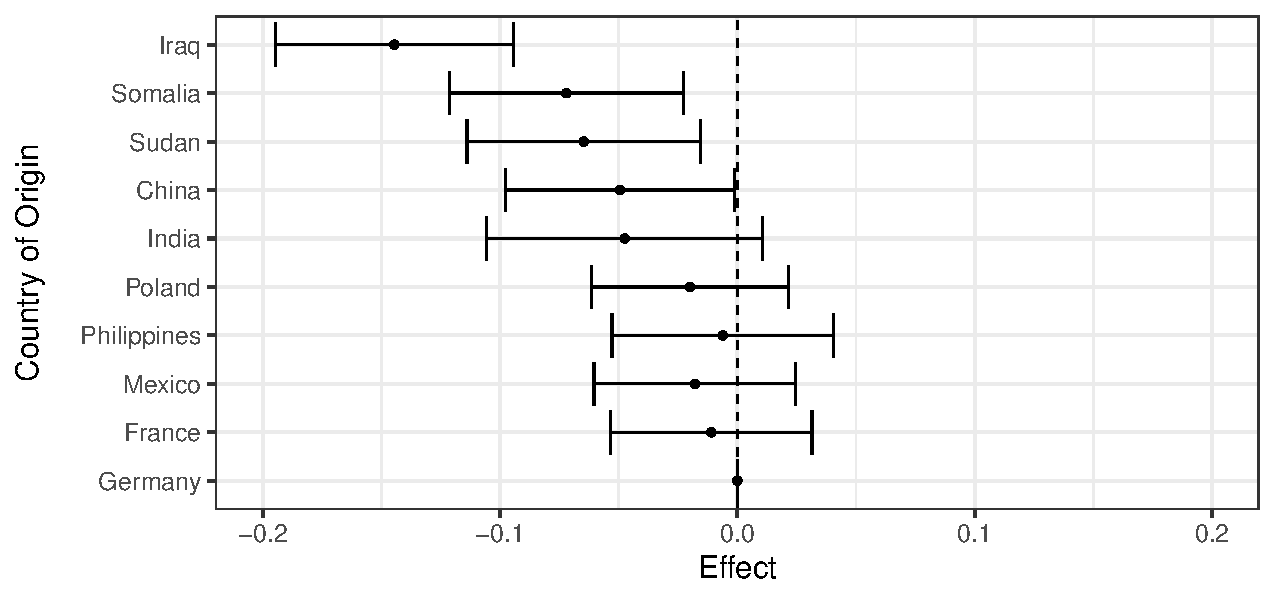
\includegraphics[width=\textwidth]{figures/hh_2015_pooled.pdf}
\caption{Estimated average marginal component effects (AMCEs) of
  country of origin where the baseline is Germany, with effect estimates as given in the original analysis of
  \cite{hainmueller2015hidden}.} \label{fig:hhy_country_est}
\end{figure}

As formalized in \cite{hainmueller2014causal}, the regression
coefficient represents the average marginal component effect (AMCE) of
each attribute averaging over all the other attributes including those
of the other profile in a given pair. 
Figure~\ref{fig:hhy_country_est} reproduces the estimated overall
AMCEs of country of origin where the baseline category is Germany.
There is little country effect with the exception of Iraq, which
negatively affects the likelihood of being preferred by a respondent.

\begin{table}[t!]
    \centering\small
    \begin{tabular}{|p{0.35\linewidth}|p{0.65\linewidth}|}
    \hline
    Moderator &Split\\
     \hline
     Education & Any college education or no college education\\
     Ethnocentrism & Median ethnocentrism measure\\
     Political party & Republican or Democrat\\
     Percent of foreign born workers in respondent's industry & High or low \\
     Household income & More or less than \$50,000\\
     Fiscal exposure to immigration & High or low\\
     ZIP code demographics & $<$ 5\% immigrants, $>$ 5\% immigrants (primarily from Latin America), or $>$ 5\% immigrants (primarily not from Latin America) \\
     Race/ethnicity & White or non-white\\
     Hispanic ethnicity & Hispanic or non-hispanic \\
     Ideology & Liberal or conservative\\
     Immigration attitudes & Supports or does not support reducing immigration\\
     Gender & Male or female \\
     Age & Young or old \\
     \hline
    \end{tabular}
    \spacingset{1}
     \caption{List of subset analyses performed in \cite{hainmueller2015hidden}, listed by moderator and how it was split to form sub-groups.}\label{tab:subsets}
\end{table}

Beyond the AMCEs, these authors and others including
\citet{newman2019economic} have explored the heterogeneous treatment
effects among respondents by conducting many sub-group analyses based
on a number of respondent characteristics including partisanship and
level of education.  Table~\ref{tab:subsets} shows all of the
sub-group analyses performed by \cite{hainmueller2015hidden} and how
the respondences were broken up into groups.  We find that 13
sub-group analyses were performed (excluding those used for robustness
checks), with results from the first three (education, ethnocentrism,
and political party) presented and discussed in the main paper.  Of
those three main analyses, the authors find some evidence of
heterogenous effects of country of origin between subsets that differ
on ethnocentrism, but little evidence of heterogeneity beyond this.
The other 10 analyses can be found in the supplemental appendix, and
the authors conclude for that participants responded similarly, in
general, across those sub-group.

Our goal is to build a methodology that enables one to more
systematically explore heterogenous treatment effects in conjoint
experiments.  Sub-group analyses like those conducted in the original
analysis can be problematic for several reasons.  First, the analyst
must conduct a separate analysis for each moderator of interest,
leading to multiple testing problem.  Second, typically the moderators
are dichotomized (or broken up into a small number of groups),
requiring the analyst to decide how to split the data.  Third, they are
not amenable to exploration of how multiple moderators might work
together to change outcomes.

To address these issues, one could include the moderators as
covariates within the regression.  However, if the goal is to provide
estimated heterogeneous effects with straightforward interpretations,
regressions with possibly complex interaction relationships are not
ideal.  The reason is that in order to estimate heterogenous effects,
we need to not only interact a large number of treatments, but we will
have to further interact all main and interaction effects of
treatments with the moderators.  It is unclear how to best reduce the
dimensionality of both the moderator and treatment space in a classic
regression set up.  Further, interpreting the interactions from these
models to understand the characteristics of units that lead to
different treatment effect patterns is challenging.

In sum, researchers must parsimoniously characterize how a large
number of possible treatment combinations interact with several key
moderators of interest.  The goal is to obtain estimates of
heterogenous effects and understand how the covariate distributions of
units with different treatment effects differ.  We now turn to our
methodology which is designed to address these challenges and result
in interpretable estimates.

 %Here, we follow \cite{newman2019economic} and focus on a
%measure of ethnic and racial prejudice by utilizing the Hispanic
%prejudice score, which represents a 0--100 point feeling thermometer
%towards Hispanics.  We dichotomize this score in the same way as
%\cite{newman2019economic}, labeling those with score below 50 as
%``high prejudice,'' and all others as ``low prejudice.''

%The results for high and low prejudice groups are shown in the right two plots of Figure~\ref{fig:hhy_country_est}.  The estimated AMCEs
%appear to suggest that respondents with low prejudice give similar
%preference to immigrants from most countries, except for Iraq and
%Somalia which are not preferred. 
%Respondents with high prejudice give less preference to immigrants from Iraq, Sudan, and Mexico. 
%However, the estimates are noisy as demonstrated by wide confidence intervals.


%Although these results suggest possible existence of heterogeneous
%treatment effects, there is a room for improved analysis.  First, it
%may be desirable to avoid dichotomization of moderator.  Second, we
%may wish to add other moderators of interest to our analysis rather
%than conducting separate subgroup analyses as done in the conjoint
%analysis literature.  When analyzing high-dimensional treatments, it
%is especially important to use a principled method for the estimation
%of heterogeneous treatment effects.  Researchers must parsimoniously
%characterize how a large number of possible treatment combinations
%interact with several key moderators of interest.  We now turn to our
%methodology which is designed to address this challenge.


\section{The Proposed Methodology}\label{sec:methods}

In this section, we describe the proposed methodology for estimating
heterogeneous effects of high-dimensional treatments.  To simplify the
exposition and notation, we focus on a general factorial design.  This
design corresponds to conjoint analysis with a single task per person\textcolor{black}{, where there is only one treatment or profile assessed rather than a comparison to two profiles,}
and the complete and independent randomization of all levels within
each factor.  The extensions to more realistic conjoint analyses are
immediate and will be discussed and applied in
Section~\ref{sec:analysis}.  

\subsection{Set Up}

Suppose that we have a simple random sample of $N$ units.  Consider a
factorial design with $J$ factors where each factor
$j \in \{1, \cdots, J\}$ has $L_j \ge 2$ levels.  The treatment
variable for unit $i$, denoted by $\bT_i$, is a $J$-dimensional vector
of random variables, each of which represents the assigned level of
the corresponding factor variable.  For example, the $j$th element of
this random vector $T_{ij} \in \{0,1,2,\ldots,L_j-1\}$ represents the
level of factor $j$ which is assigned to unit $i$.

Following \cite{DasPilRub15}, we define the potential outcome for unit $i$ as
$Y_i(\bt)$ where $\bt \in \cT$ represents the realized treatment with
$\cT$ representing the support of the randomization distribution for
$\bT_i$.  Then, the observed outcome is given by $Y_i = Y_i(\bT_i)$.
The notation implicitly assumes no interference between units
\citep{Rubin80}.  In this paper, for the sake of concreteness, we
focus on the binary outcome $Y_i \in \{0, 1\}$.  Extensions to
non-binary outcomes are straightforward.  Lastly, we observe a vector
of $p_x$ pre-treatment covariates for each unit $i$ and denote it by
$\bX_i$.
All together, we observe $(Y_i, \bT_i, \bX_i)$ for each unit $i$.

To illustrate the notation, consider a simplified version of our motivating example where each participant $i$ observes a single immigrant profile and must decide whether to support that immigrant's admission or not.
Then $\bT_i$ is a vector indicating the level participant $i$ sees for each of the nine immigrant attributes.
$Y_i$ is an indicator for whether participant $i$ chooses to support admission for the immigrant they are presented with.
$\bX_i$ is a vector of covariates for participant $i$ that we believe might moderate the treatment effect (i.e., we believe there may be treatment effect heterogeneity based on the $\bX_i$).
In our example, $\bX_i$ included political party, education, demographics of their ZIP code, ethnicity, and Hispanic prejudice score (see Section~\ref{sec:analysis:data_model} for more details on how these variables were defined).

The randomness in our data, $(Y_i, \bT_i, \bX_i)$ comes from two sources: random sampling of units into the study and random assignment of units to treatments.
For simplicity, we assume units are sampled via simple random sampling (though this can be relaxed and survey weights incorporated into our method).
We further assume that the design used to randomize the assignment of of treatment is such that
\begin{equation*}
  \{Y_i(\bt)\}_{\bt \in \cT} \ \ind \  \bT_i
\end{equation*}
for each $i$ (this will hold for common designs where all units have the same probabilities of receiving each treatment).
The exact mode of randomization will determine the distribution of $\bT_i$.
In many practical applications of conjoint analysis,
researchers independently and uniformly randomize each factor.
However, in some cases including our application, researchers may
exclude certain unrealistic combinations of factor levels (e.g.,
doctor without a college degree), leading to the dependence between
factors.  In all cases, researchers have complete knowledge of the
randomization distribution of the factorial treatment variables.

Based on random sampling and random treatment assignment alone, we can conduct valid inference for treatment effects of interest using basic regression or difference of means.
However, if we wish to explore heterogeneity in responses to treatments, a model-based approach is useful.
We next introduce our model, which will allow us to explore heterogeneous effects in a principled manner while also handling the high-dimensional nature of the data.


\subsection{Modeling Heterogeneous Treatment Effects}

The most basic causal quantity of interest is the average marginal
component effect \citep[AMCE;][]{hainmueller2014causal}, which is
defined for any given factor $j$ as,
\begin{equation}
  \delta_j (l, l^\prime) \ = \ \E\{Y_i(T_{ij}=l, \bT_{i,-j}) - Y_i(T_{ij}
  = l^\prime, \bT_{i,-j})\}, \label{eq:AMCE}
\end{equation}
where $l \ne l^\prime \in \cT_j$ with $\cT_j$ representing the support
of the randomization distribution for $T_j$.  The expectation in
Equation~\eqref{eq:AMCE} is taken over the distribution of the other
factors $\bT_{i,-j}$ as well as the random sampling of units from the
population.  Thus, the AMCE averages over two sources of causal
heterogeneity --- heterogeneity across treatment combinations and
across units.  Different treatment combinations may have distinct
impacts on units with varying characteristics.  Our goal is to model
these potentially complex heterogeneous treatment effects using an
interpretable model.

%We propose to use a (Bayesain) mixture of experts based on a small number of regularized logistic regressions \citep[see][for a recent review]{gormley2019mixture}.
We propose to use a (Bayesain) mixture of experts based on a small number of regularized logistic regressions.
Mixture of experts models are conditional mixture models in which one model determines the weights given to each cluster (or component) and each cluster has a separate model for the outcome (the ``expert'') \citep[see][for a recent review]{gormley2019mixture}. After estimation, there is a set of interpretable clusters with different treatment effects as well as a mapping from pre-treatment covariates to cluster membership probabilities. For our empirical example, we might recover two-cluster results similar to those shown in Figure~\ref{fig:hhy_country_est}, where, for example, cluster 1 corresponds to highly prejudiced individuals and cluster 2 corresponds to low prejudice individuals.
The model consists of two parts.  First,
for each cluster, a regularized logistic regression is used to model
the outcome variable as a function of treatments $\bT_i$ where an
ANOVA-style sum-to-zero constraint is imposed separately for each
factor.  Regularization is used to facilitate merging of different
levels within each factor.  This modeling strategy identifies a
relatively small number of treatment combinations while avoiding the
specification of a baseline level for each factor
\citep{egam:imai:19}. Second, we model the probability of unit $i$'s
assignment to each cluster using a set of $p_x$ unit characteristics
$\bX_i$.
 We refer to $\bX_i$ as ``moderators.''
 These moderators describe the characteristics of units that belong to each cluster.
All together, the proposed modeling strategy allows researchers to identify interpretable patterns of heterogeneous effects across treatment combinations and units.
Our model is conditional on the $\bX_i$ and $\bT_i$.

Formally, let $K$ be the number of clusters.  Then, the model is
defined as follows,
\begin{equation}
\label{eq:unreg}
\Pr(Y_i = 1 \mid \bT_i, \bX_i) \ = \   \sum_{k=1}^K \pi_{k}(\bX_i)
\zeta_{k}(\bT_i) 
\end{equation}
where $i=1,2,\ldots,N$ and for $k=1,2,\ldots,K$, we use the logistic
regression to model the outcome variable and the multinomial logit
model for the cluster membership,
\begin{equation}
  \zeta_{k}(\bT_i) \
= \ \frac{\exp(\psi_{k}(\bT_i))}{1+\exp(\psi_{k}(\bT_i))}, \quad
\text{and} \quad
\pi_{k}(\bX_i) = \frac{\exp(\bX_i^\top \bphi_k)}{\sum_{k'=1}^K
  \exp(\bX_i^\top \bphi_{k'})}. \label{eq:basic_models}
\end{equation}
For identification, we set $\bphi_1 = \bzero$.

We use the following linear equation for $\psi_{k}(\bT_i)$ where we
include both main effects and two-way interaction effects with a
common intercept $\mu$ shared across all clusters,
\begin{align*}
\psi_{k}(\bT_i)& \ =\ \mu + \sum_{j=1}^J \sum_{l =0}^{L_j-1} 
\mathbf{1}\{T_{ij} = l\} \beta^j_{kl} + \sum_{j=1}^{J-1} \sum_{j' >
  j} \sum_{l=0}^{L_j-1} \sum_{l' = 0}^{L_{j'}-1} \mathbf{1}\{T_{ij} = l,
T_{ij'} = l'\} \beta^{jj'}_{kll'}\\
&\ =\ \mu + \bm{t}_i^\top\bbeta_k, 
\end{align*}
for each $k=1,2,\ldots,K$ where $\bm{t}_i$ is the vector of
indicators, $\mathbf{1}\{T_{ij} = l\}$ and
$\mathbf{1}\{T_{ij} = l, T_{ij'} = l'\}$, and $\bbeta_k$ is a stacked
column vector containing all coefficients for cluster $k$.  We use the
following ANOVA-type sum-to-zero constraints,
\begin{equation}
  \sum_{l =0}^{L_j-1} \beta^j_{kl} = 0, \quad \text{and} \quad
  \sum_{l=0}^{L_{j}-1} \beta^{jj'}_{kll'} = 0, \label{eq:sum-to-zero}
\end{equation}
for each $j,j'=1,2,\ldots,J$ with $j' > j$, and
$l'=0,1,\ldots,L_{j'}$. 

We write these constraints compactly as,
\begin{equation}
  \bC^\top \bbeta_k \ = \ \bm{0}. \label{eq:constraint}
\end{equation}
Each row of $\bC^\top \bbeta_k$
corresponds to one of the sum-to-zero constraints given in
Equation~\eqref{eq:sum-to-zero}.  For example, in a model without
interactions, $\bm{C}$ takes the following $J \times \sum_{j=1}^J L_j$
matrix,
\begin{equation*}
  \bC \ = \ \begin{bmatrix} \bm{1}_{L_1} & \bm{0}_{L_2} & \cdots &
    \bm{0}_{L_J}
    \\ \bm{0}_{L_1} & \bm{1}_{L_2} & \cdots & \bm{0}_{L_j} \\
    \vdots & \vdots & \ddots & \vdots \\ \bm{0}_{L_1} &
    \bm{0}_{L_2}
    & \cdots &
    \bm{1}_{L_J}
  \end{bmatrix}, 
\end{equation*}
where $\bzero_p$ and $\bone_p$ denote the column vectors of zeros and
ones, respectively, with length $p$.  

\subsection{Sparsity-induced Prior}

Given the high dimensionality of this model, we use a
sparsity-inducing prior.  For example, in our application, we have 315
$\beta$ parameters for each cluster.  In factorial experiments, it is
desirable to regularize the model such that certain levels of each
factor are fused together when their main effects and all interactions
are similar \citep{post2013factor,egam:imai:19}.  For example, we
would like to fuse levels $l_1$ and $l_2$ of factor $j$ if
$\beta^j_{l_1} \approx \beta^j_{l_2}$ and
$\beta^{jj'}_{l_1 l'} \approx \beta^{jj'}_{l_2 l'} $for all other
factors $j'$ and all of its levels $l'$.
% A key problem with the above approach is that the model may be high
% dimensional and thus requires regularization to provide stable
% results. Existing work in the non-factorial case has focused on
% using a sparsity-inducing penalty (LASSO, SCAD;
% e.g. \citealt{stadler2010lasso,khal:chen:07,chamroukhi2019regularized})
% and some results on the oracle properties of such estimators have
% been derived
% (e.g. \citealt{stadler2010lasso,khalili2010mixture,nguyen2021lasso}).

We encourage such fusion by applying a structured sparsity approach of
\citet{goplerud2021sparsity} that generalizes the group and
overlapping group LASSO
\citep[e.g.,][]{yuan:lin:06,yan2017hierarchical} while allowing
positive semi-definite constraint matrices.  For computational
tractability, we use $\ell_2$ norm instead of the $\ell_\infty$ norm,
which is used in GASH-ANOVA \citep{post2013factor}.

To build an intuition, consider a simple example with a single cluster
and two factors---factor one has three levels and factor two has two
levels.  In this case, our penalty contains four terms,
\begin{equation*}
\begin{split}
& \sqrt{(\beta^1_0 - \beta^1_1)^2 +  (\beta^{12}_{00} -
    \beta^{12}_{10})^2 + (\beta^{12}_{01} -
    \beta^{12}_{11})^2}\\
  ~+~ &\sqrt{(\beta^1_0 - \beta^1_2)^2 +
    (\beta^{12}_{00} - \beta^{12}_{20})^2 +
    (\beta^{12}_{01}-\beta^{12}_{21})^2}\\
~+~ & \sqrt{(\beta^1_1 - \beta^1_2)^2 + (\beta^{12}_{10} - \beta^{12}_{20})^2 + (\beta^{12}_{11} - \beta^{12}_{21})^2}\\
~+~ & \sqrt{(\beta^2_0 - \beta^2_1)^2 +  (\beta^{12}_{00}-\beta^{12}_{01})^2 + (\beta^{12}_{10} - \beta^{12}_{11})^2 + (\beta^{12}_{20}-\beta^{12}_{21})^2} .
\end{split}
\end{equation*}
The first three terms encourages the pairwise fusion of the levels of
factor one whereas the fourth encourages the fusion of the two levels
of factor two. For compact notation, the penalty can also be written
using the sum of Euclidean norms of quadratic forms,
\begin{equation*}
 || \bm{\beta}^\top \bm{F}_1 \bm{\beta} ||_2 +  \ ||
 \bm{\beta}^\top \bm{F}_2 \bm{\beta} ||_2 + \ ||
 \bm{\beta}^\top \bm{F}_3 \bm{\beta} ||_2 + \ ||
 \bm{\beta}^\top \bm{F}_4 \bm{\beta} ||_2,  
\end{equation*}
where $\bF_1, \bF_2, \bF_3$ are appropriate positive semi-definite
matrices to encourage the fusion of the pairs of levels in factor one
and $\bF_4$ encourages the fusion of the two factors in factor two,
and
$\bbeta = [\beta^1_0\ \beta^1_1\ \beta^1_2\ \beta^2_0\ \beta^2_1\
\beta^{12}_{00}\ \beta^{12}_{10}\ \beta^{12}_{20}\ \beta^{12}_{01}\
\beta^{12}_{11}\ \beta^{12}_{21}]^\top$.
Note that the sum to zero constraints make this type of fusion of factors together sensible for sparsity. 

We generalize this formulation to an arbitrary number of factors and
factor levels. For each factor that contains $L_j$ levels, we have
$\binom{L_j}{2}$ penalty matrices to encourage pairwise
fusion. Imposing additional constraints, e.g. for ordered factors, is
a simple extension. Let $G = \sum_{j=1}^J \binom{L_j}{2}$ represent
the total number of penalty matrices.  For $g=1,2,\ldots,G$, we use
$\bF_g$ to denote a penalty matrix such that
$\sqrt{\bbeta^\top\bF_{g}\bbeta}$ is equivalent to the $\ell_2$ norm
on the vector of differences between all main effects and interactions
containing a main effect.

We cast this penalty as the following Bayesian prior distribution so
that our inference is based on the posterior distribution given the conditional prior on $\bm{\beta}_k$,
\begin{equation}
\label{eq:prior_beta}
p\left(\bbeta_k \mid \{\bm{\phi}_k\}_{k=2}^K\right) \ \propto \ \left(\lambda {\bar{\pi}_k^\gamma}\right)^m \exp\left(-\lambda \bar{\pi}_k^\gamma \sum_{g=1}^{G} \sqrt{\bbeta_k^\top\bF_{g} \bbeta_k}\right), 
\end{equation}
where $\bar{\pi}_k = \sum_{i=1}^N \pi_k(\bX_i)/N$ and
$m = \text{rank}\left([\bF_{1}, \cdots, \bF_{G}]\right)$. We follow
existing work in allowing the penalty on the treatment effects
$\bm{\beta}_k$ to be scaled by the cluster-membership size
$\bar{\pi}_k$ when $\gamma = 1$
\citep{khal:chen:07,stadler2010lasso}.
On the other hand, when $\gamma = 0$ the $\bar{\pi}_k$ disappears, implying no use of the $\bX_i$ in the prior.
 We note that the prior on
$p(\bm{\beta} \mid \{\bm{\phi}_k\}_{k=2}^K)$ is guaranteed to be
proper when all pairwise fusions are encouraged by
$\{\bm{F}_g\}_{g=1}^G$, although in other circumstances it may be
improper
\citep{goplerud2021sparsity}.  Appendix~\ref{sec:app_ssparse_prior}
provides additional details. Following \cite{zahid2013ridge}, we use a
normal prior distribution for the coefficients for the moderators.

The resulting regularization is invariant to the choice of baseline
category $\bphi_1 = \bm{0}$, which is the first row of the
$K \times p_x$ coefficient matrix $\bphi$.  The prior distribution is
given by,
\begin{equation}
\label{eq:prior_phi}
p(\{\bm{\phi}_k\}_{k=2}^K) \ \propto \ \exp\left(-\frac{\sigma^2_\phi}{2}\sum_{l=1}^{p_x} [\bphi_{2l}, \cdots, \bphi_{Kl}]^\top \bm{\Sigma}_\phi [\bphi_{2l}, \cdots, \bphi_{Kl}]\right), 
\end{equation}
where $\bm{\Sigma}_\phi$ is a $(K-1) \times (K-1)$ matrix with
$[\bm{\Sigma}_\phi]_{kk'} = (K-1)/K$ if $k = k'$ and $[\bm{\Sigma}_\phi]_{kk'} =-1/K$
otherwise. We set $\sigma^2_\phi$ to $1/4$ for a relatively diffuse prior.

As noted in a recent survey, ``ensuring generic identifiability for general [mixture of expert] models remains a challenging issue'' \cite[p. 294]{gormley2019mixture}.  Although mixtures with a Bernoulli outcome variable are generally unidentifiable, several aspects of our methodology are expected to alleviate the identifiability problem. First, a typical conjoint analysis has repeated observations per unit $i$ \citep{grun2008multinomial}.  Second, our model is a mixture of experts rather than a mixture model \citep{jiang1999identifiability}.
Third, our covariates are randomized. Finally, our model regularizes the coefficients through an informative prior. Unfortunately, a formal identifiability analysis of our model is beyond the scope of this paper.  Our simulation analysis (Section~\ref{sec:simulation}), however, shows that our model can accurately recover the coefficients in a realistic setting for applied research. It is also possible to use a bootstrap-based procedure to examine the
identifiability issue in a specific setting
\citep{grun2008multinomial}.


\subsection{Estimation and Inference}

We fit our model by finding a maximum of the log-posterior using an
extension of the Expectation-Maximization (EM;
\citealt{demp:lair:rubi:77}) known as the Alternating
Expectation-Conditional Maximization (AECM;
\citealt{meng:vand:97}). Equation~\eqref{eq:aecm_obs} defines our
(observed) log-posterior using the terms defined in
Equations~\eqref{eq:unreg},~\eqref{eq:prior_beta},
and~\eqref{eq:prior_phi}, where we collect all model parameters as
$\bm{\theta}$.
\begin{equation}
\label{eq:aecm_obs}
\ln p(\bm{\theta} | \{Y_i\}) \propto \sum_{i=1}^N \ln\left(\sum_{k=1}^K \pi_{k}(\bX_i) \zeta_k(\bT_i)\right) + \sum_{k=1}^K \ln p(\bm{\beta}_k | \{\bm{\phi}\}_{k=2}^K) + \ln p(\{\bm{\phi}_k\}_{k=2}^K)
\end{equation}

For now, we assume the value of regularization parameter $\lambda$ is
fixed, although we discuss this issue in
Section~\ref{sec:additional}. The linear constraints on $\bm{\beta}_k$
given in Equation~\eqref{eq:constraint} still hold but are suppressed
for notational simplicity; we return to this point at the end of this
subsection.

Algorithm~\ref{alg:main} summarizes our approach to finding a maximum
of Equation~\eqref{eq:aecm_obs}.  Each iteration of our AECM algorithm
involves two ``cycles'' where the data augmentation scheme enables
iterative updating of the treatment effect parameters $\bm{\beta}$ and
moderators $\bm{\phi}$.

\begin{algorithm}[!t]\spacingset{1.25}
	\caption{AECM Algorithm for Estimating $\bm{\theta}$}
	\label{alg:main}
	\begin{algorithmic}
		\State{\textbf{Set Hyper-Parameters}: $K$ (clusters), $\lambda$, $\sigma^2_\phi$, $\gamma$ (prior strength), $\epsilon_1, \epsilon_2$ (convergence criteria), $T$ (number of iterations)}
		
		\State{\textbf{Initialize Parameters}: $\bm{\theta}^{(0)}$, i.e. $\bm{\beta}^{(0)}$ and $\bm{\phi}^{(0)}$; Appendix~\ref{sec:app_derivations_improve} provides details.}
		\For{iteration $t \in \{0, \cdots, T-1\}$}
		\State{\textbf{Cycle 1: Update $\bm{\beta}$}}
		\State{1a.} $E$-Step: Find the conditional distributions of $\{Z_i, \omega_i\}_{i=1}^N$ and $\{\{\tau^2_{gk}\}_{g=1}^G\}_{k=1}^K$ given $\{Y_i\}$ and $\bm{\theta}^{(t)}$ (Eq.~\eqref{eq:aecm_ebeta}). Derive $Q_\beta(\bm{\beta}, \bm{\theta}^{(t)})$ (Eq.~\eqref{eq:aecm_qbeta}).
		\State{1b.} $M$-Step: Set $\bm{\beta}^{(t+1)}$ such that $Q_\beta(\bm{\beta}^{(t+1)}, \bm{\theta}^{(t)}) \geq Q_\beta(\bm{\beta}^{(t)}, \bm{\theta}^{(t)})$ 
		\State{\textbf{Cycle 2: Update $\bm{\phi}$}}
		\State{2a.} $E$-Step: Find $p(Z_i=k\mid~Y_i, \bm{\beta}^{(t+1)}, \bm{\phi}^{(t)})$. Derive $Q_\phi(\bm{\phi}, \{\bm{\beta}^{(t+1)}, \bm{\phi}^{(t)}\})$ (Eq.~\eqref{eq:aecm_qphi}). 
		\State{2b.} $M$-Step: Set $\bm{\phi}^{(t+1)}$ such that 
		
		$Q_\phi(\bm{\phi}^{(t+1)}, \{\bm{\beta}^{(t+1)}, \bm{\phi}^{(t)}\}) \geq Q_\phi(\bm{\phi}^{(t)}, \{\bm{\beta}^{(t+1)}, \bm{\phi}^{(t)}\})$
		\State{\textbf{Check Convergence}}
		\State{3.} Stop if $\ln p(\bm{\theta}^{(t+1)} | \{Y_i\}) - \ln p(\bm{\theta}^{(t)} | \{Y_i\}) < \epsilon_1$ (Eq.~\eqref{eq:aecm_obs}) or $||\bm{\theta}^{(t+1)} - \bm{\theta}^{(t)}||_\infty < \epsilon_2$.
		\EndFor
	\end{algorithmic}
\end{algorithm}

To update $\bm{\beta}$, our data augmentation strategy requires three
types of missing data.  First, we use the standard cluster memberships of each
unit $i$ for inference in finite mixtures, i.e.,
$Z_i \in \{1, \cdots, K\}$.  We also include two other types of data
augmentation that result in a closed-form update for $\bm{\beta}$.  We
use Polya-Gamma augmentation ($\omega_i$;
\citealt{polson2013polyagamma}) for the logistic likelihood and data
augmentation on the sparsity-inducing penalty ($\tau^2_{gk}$; see,
e.g.,
\citealt{figueiredo2003adaptive,polson2011svm,ratkovic2017sparse,goplerud2021sparsity}).
\begin{subequations}
\label{eq:aecm_ebeta}
\begin{align}
&p(Y_i, \omega_{i} \mid Z_i) \ \propto \ \frac{1}{2}\exp\left\{\left(Y_i - \frac{1}{2}\right) \psi_{Z_i}(\bT_i) - \frac{\omega_{i}}{2} \left[\psi_{Z_i}(\bT_i)\right]^2\right\} f_{PG}(\omega_{i} \mid 1, 0),\label{eq:augmented1} \\
&p(\bm{\beta}_k, \{\tau^2_{gk}\}_{g=1}^G \mid \lambda,
\{\bm{\phi}_k\}) \ \propto \
\exp\left\{-\frac{1}{2}\bm{\beta}_k^\top\left(\sum_{g=1}^G
\frac{\bm{F}_{g}}{\tau^2_{gk}}\right)
\bm{\beta}_k\right\} \prod_{g=1}^G\tau_{gk}^{-1}
\exp\left\{-\frac{\left(\lambda \bar{\pi}_k\right)^2}{2} \cdot \tau^2_{gk}\right\} \label{eq:augmented2}
\end{align}
\end{subequations}
where $f_{PG}(\cdot \mid b, c)$ represents the Polya-Gamma
distribution with parameters $(b,c)$ and
$Z_i \sim \mathrm{Multinomial}\left(1, \bm{\pi}_i\right)$ with the
$k$th element of $\bm{\pi}$ equal to $\pi_k(\bX_i)$. Note that
$\bm{\beta}$ only enters Equation~\eqref{eq:aecm_ebeta} via a
quadratic form.

The first cycle of the AECM algorithm involves, therefore, maximizing
or improving the following $Q$-function with respect to $\bm{\beta}$
given $\bm{\theta}^{(t)}$.
\begin{align}
\label{eq:aecm_qbeta}
Q_\beta\left(\bm{\beta}, \bm{\theta}^{(t)}\right)\ = \ &\sum_{i=1}^N \sum_{k=1}^K \E(\mathbf{1}\{Z_i = k\})\left\{\left(Y_i -
\frac{1}{2}\right) \psi_{k}(\bT_i) - \E(\omega_i \mid Z_i = k)
\frac{\left[\psi_k(\bT_i)\right]^2}{2}\right\}  \nonumber \\
                                                  & + \sum_{k=1}^K -\frac{1}{2}
\bm{\beta}_k^\top \left[\sum_{g=1}^K \bm{F}_g \cdot
\E(1/\tau^2_{gk})\right] \bm{\beta}_k + \text{const.}
\end{align}
where all expectations are taken over the conditional distribution of
the missing data given the current parameter estimates.  We note that
the $E$-Step involves computing
$p(\{\omega_i, Z_i\}, \{1/\tau^2_{gk}\} | \{Y_i\}, \bm{\theta}^{(t)})$
which factorizes into, respectively, a collection of Polya-Gamma,
categorical, and Inverse-Gaussian random variables
(Appendix~\ref{sec:app_derivation_EM} provides the full conditional
distributions and all relevant expectations).  Thus, maximizing
$Q_\beta$ reduces to a linear ridge regression for $\bm{\beta}$.

Lastly, updating $\bm{\beta}$ requires incorporating the constraint
defined in Equation~\eqref{eq:constraint}.  The constraint implies
that $\bbeta_k$ belongs to the null space of $\bC^\top$
\citep{lawson1974linear}. Let $\mathcal{B}_{\bC^\top}$ represent a
basis of the null space of $\bC^\top$. Rather than performing
inference directly on $\bbeta_k$ in the constrained space, we consider
unconstrained inference on the transformed parameter
$\tilde{\bbeta}_k \in \mathbb{R}^{\text{rank}(\bC^\top)}$ where
$\tilde{\bbeta}_k=\left(\mathcal{B}_{\bC^\top}^\top
  \mathcal{B}_{\bC^\top}\right)^{-1}
\mathcal{B}_{\bC^\top}^\top\bbeta_k $.  Similarly, we re-define
$\bF_g$ as $\mathcal{B}_{\bC^\top}^\top \bF_g
\mathcal{B}_{\bC^\top}$. Once the algorithm converges, the constrained
parameters $\bbeta_k$ are obtained noting
$\bbeta_k = \mathcal{B}_{\bC^\top}
\tilde{\bbeta}_k$. Appendix~\ref{sec:app_derivation_LC} provides a
full derivation of the removal of the linear constraints.


To update the moderator parameters $\bphi$, we use the second cycle of
the AECM algorithm where only the $Z_i$ are treated as missing
data. The $E$-step involves recomputing the cluster memberships, i.e.,
$p(Z_i \mid Y_i, \bm{\beta}^{(t+1)}, \bm{\phi}^{(t)})$, given the updates in the first
cycle. The implied $Q$-function is shown below,
\begin{align}
\label{eq:aecm_qphi}
Q_{\phi}(\bm{\phi}, \{\bm{\beta}^{(t+1)}, \bm{\phi}^{(t)}\}) \ = \
&\sum_{k=1}^K \left[\sum_{i=1}^N \E(\mathbf{1}\{Z_{i} = k\})\ln(\pi_{k}(\bX_i))\right] \nonumber \\
& + \sum_{k=1}^K \left[m \gamma \ln(\bar{\pi}_k) - \lambda \bar{\pi}_k^\gamma \sum_{g=1}^{G} \sqrt{\bbeta_k^\top \bF_{g} \bbeta_k}\right] + \ln p(\{\bphi_k\}_{k=2}^K),
\end{align}
where $\pi_k(\bX_i)$ and $\bar\pi_k= \sum_{i=1}^N \pi_k(\bX_i)/N$ are
functions of $\bphi_k$.  Note that if $\gamma = 0$, this simplifies to
a (weighted) multinomial logistic regression with $\E(z_{ik})$ as the
outcome. We perform the $M$-Step by using a few steps of a standard
optimizer (e.g., L-BFGS-B) to increase $Q_{\phi}$ and thus obtain
$\bm{\phi}^{(t+1)}$.


\subsection{Additional Considerations}
\label{sec:additional}

Since fitting the proposed model is computationally expensive, we use
an information criterion approach based on BIC, rather than cross
validation, to select the value of the regularization parameter
$\lambda$
\citep{khal:chen:07,khalili2010mixture,chamroukhi2019regularized}. Appendix~\ref{sec:app_derivations_df}
presents our degrees-of-freedom estimation and explains how we tune
$\lambda$ using Bayesian model-based
optimization. Appendix~\ref{sec:app_derivations_improve} discusses
additional details of our EM algorithm including initialization and
techniques to accelerate convergence.

We extend the above model and estimation algorithm to accommodate
common features of conjoint analysis: (1) repeated observations for
each individual respondent (Appendix~\ref{sec:app_extensions_repeat}),
(2) a forced choice conjoint design
(Appendix~\ref{sec:app_extensions_forced}), and (3) standardization
weights for factors with different numbers of levels $L_j$
(Appendix~\ref{sec:app_extensions_standardization}). Lastly, our
experience suggests that the proposed penalty function, which consists
of overlapping groups, often finds highly sparse
solutions. Appendix~\ref{sec:app_log} details the integration of the
latent overlapping group formulation of \cite{yan2017hierarchical}
into our framework to address this issue.

Once the model parameters are estimated, we can compute quantities of
interest such as the AMCEs, defined in Equation~\eqref{eq:AMCE}.  We
do this separately for each cluster, such that
$\delta_{jk} (l, l^\prime)$ is the AMCE for factor $j$, changing from
level $l^{\prime}$ to $l$ in cluster $k$.  Our estimator is the
average of the estimated difference in predicted responses when
changing from level $l^{\prime}$ to $l$ of factor $j$, where the
average is taken over the empirical distribution of the assignment on
the other factors.  This estimation is described in more detail in
Appendix~\ref{append:amce_acie_der}: Appendix~\ref{append:amce_fac}
discusses factorial designs (with or without randomization
restrictions) whereas Appendix~\ref{append:amce_conjoint} discusses
forced-choice conjoint designs (with or without randomization
restrictions).  We can use the empirical distribution here because
treatment is randomly assigned.

To quantify the uncertainty of the parameter estimates, we rely on a
quadratic approximation to the log posterior distribution. To ensure
its differentiability, we follow a standard approach in the
regularized regression literature \citep[e.g.,][]{fan2001variable} and 
fuse pairwise factor levels that are sufficiently close
together. Appendix~\ref{sec:app_uncertainty} describes this process,
with Appendix \ref{append:hess} and \ref{append:hes_rep_obs} deriving
the Hessian of the log-posterior using \cite{loui:82}'s method; we
then use the Delta method, as described in
Appendix~\ref{append:uncert_delta}, for inference on other of
quantities of interest, e.g. the AMCE.


\section{Simulations}\label{sec:simulation}

We explore the performance of our method using a simple but realistic
simulation study.  Specifically, we consider the case of a conjoint
experiment with ten factors ($J = 10$) each with three levels
($L_j = 3$). To evaluate the performance of the proposed method, we
consider two different settings; in the first, we assume there are
1,000 respondents who each perform five comparison tasks. In the
second, we assume a larger experiment with 2,000 respondents who each
perform ten tasks.

In all cases, we assume the true data generating process has three
distinct clusters $K = 3$ and we calibrate the true $\bm{\beta}_k$
such that the implied average marginal component effects (AMCE) are comparable in
magnitude to the empirical effects presented in
Section~\ref{sec:analysis}. We use a set of six correlated continuous
moderators to again mimic a realistic empirical setting and choose
$\{\bm{\phi}_k\}_{k=2}^3$ to relatively clearly separate respondents into different clusters.  Appendix~\ref{sec:app_simulations} presents complete
description of the simulation settings and the true parameter values
used for the $\bm{\beta}_k$ and marginal effects.

For each sample size, we independently generate 1,000 simulation data
sets by drawing $N$ observations of moderators, randomly assigning a
true cluster membership to each observation based on the implied
probabilities given their moderators, and generating the observed
profiles completely at random. We fit our model to the data with
$K = 3$ and examine the average marginal component effects with respect to the
first baseline level (see Appendix~\ref{sec:app_simulations_coverage}
for the results regarding the estimated coefficients $\bm{\beta}_k$).

\begin{figure}[!t]
  \centering \spacingset{1}
  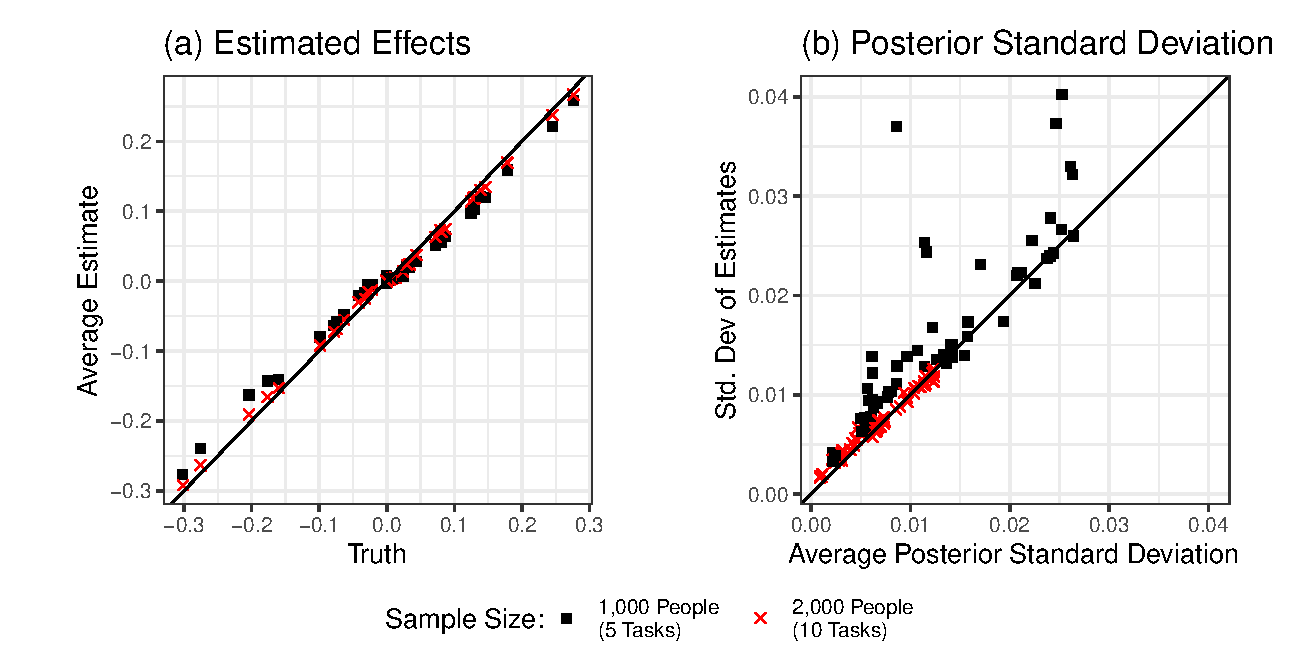
\includegraphics[width=\textwidth]{figures/sim_ame.eps}
  \caption{The empirical performance of the proposed estimator on
    simulated data. The black squares indicate the effects estimated
    with the smaller sample size (1,000 people completing 5 tasks);
    the red crosses indicate effects estimated with the larger sample
    size (2,000 people completing 10 tasks).}
  \label{fig:simulation}
\end{figure}

Figure~\ref{fig:simulation} summarizes our results. The left panel
illustrates a high correlation between the estimated effects and their true values ($\rho = 0.995$ for smaller sample size; $\rho = 0.999$ for larger sample size). While the performance overall is reasonably strong, we see that even when the dataset is large there is some degree of attenuation bias due to shrinkage.

The right panel illustrates the frequentist evaluation of our Bayesian
posterior standard deviations.  We compare the average posterior
standard deviation against the standard deviation of the estimated
effects across the 1,000 Monte Carlo simulations.  The average
posterior standard deviations are noticeably smaller than the standard
deviation of the estimates when the sample size is small.  For the
large sample size, however, there is a much closer relationship.
Thus, given sufficiently large data, our approximate Bayesian
posterior standard deviations in this simulated example are roughly
the same magnitude of the standard deviation of the sampling
distribution of the estimator. Even though our method's frequentist
coverage is somewhat below the nominal level (see
Appendix~\ref{sec:app_simulations_coverage}), this undercoverage
appears to be primarily attributable to the shrinkage bias in our
regularized estimation procedure rather than the large sample
discrepancy between our posterior standard deviations and the
corresponding standard deviation of sampling distribution.

Appendix~\ref{sec:app_simulations_coverage} explores one way to
address the limitations of the default estimator by exploring sample
splitting and refitting the model given the estimated sparsity pattern
(i.e., which levels are fused together) and moderator effects
($\{\bm{\phi}_k\}_{k=2}^K$) on half of the data. This results in
smaller bias and improved coverage at both sample sizes. 

\section{Empirical Analysis}\label{sec:analysis}

In this section, we re-analyze the immigration conjoint data
introduced in Section~\ref{sec:con}, using our methodology.  We find
evidence of effect heterogeneity for immigrant choice based on
respondents traits.  In particular, we consistently find that the
immigrant's country of origin plays a greater role in forming the
immigration preference of respondents with increased prejudice, as
measured by a Hispanic prejudice score.  However, outside of this
cluster, which accounts for about one third or more of the
respondents, the country of origin factor plays a much smaller role. 

\subsection{Data and Model}\label{sec:analysis:data_model}

Following the original analysis, our model includes indicator variables
for each factor and interactions between country and reason of
application factors as well as those between education and job factors
in order to account for the restricted randomization.  We additionally
include interactions between country and job as well as those between
country and education, in accordance with the skill premium theory of
\cite{newman2019economic}.  This theory hypothesizes that prejudiced
individuals prefer highly skilled immigrants only for certain
immigrant countries.  This results in a total of 41 AMCEs and 222
AMIEs for each cluster.

For modeling cluster membership, we include the respondents' political
party, education, demographics of their ZIP code (we follow the
original analysis and include the variables indicating whether
respondents' ZIP code had few immigrants ($<5\%$) and for those from
ZIPs with more than $5\%$ foreign-born, whether the majority were from
Latin America), ethnicity, and Hispanic prejudice score.  The Hispanic
prejudice score was used by \cite{newman2019economic}, though we
negate it to make lower values correspond to lower prejudice for
easier interpretation.  The score is based on a standardized (and
negated) feeling thermometer for Hispanics.  The score ranges from
$-1.61$ to $2.11$ for our sample, where higher scores indicate higher
levels of prejudice.

% \cite{newman2019economic} found similar results for using the
% Hispanic feeling thermometer alone as in combination with the
% feeling thermometer for ``immigrants.''  They also argue that this
% is a more relevant measure of prejudice than the ethnocentrism score
% used in \cite{hainmueller2015hidden}, because it does not include
% the in-group feeling thermometer.  It also does not include the
% feeling thermometer for ``Asians'', which the ethnocentrism score
% from \cite{hainmueller2015hidden} does.  We chose this set of
% moderator variables as substantively they appear to be the most
% relevant and likely to modify effects.

We remove respondents who are Hispanic since the Hispanic prejudice
score, which is our moderator, was not measured for these respondents.
After removing entries with missing data, we have a sample of 1,069
respondents. Most respondents evaluated five pairs of profiles, though
five respondents have fewer responses in the data set used.  The total
number of observations is, therefore, 5,337 pairs of profiles.  We do
not incorporate the survey weights into our analysis to better
demonstrate our methods without adding extra variability due to
potentially noisy weights.

The original conjoint experiment was conducted using the forced choice
design, in which a pair of immigrant profiles are presented and a
respondent is asked to choose one of them. To accommodate this design,
we follow \cite{egam:imai:19} and slightly modify the model
specification.  In particular, we model the choice as a function of
differences in treatments as follows,
\begin{align*}
\psi_k(\bT_i^L, \bT_i^R) \ = \ &  \mu + \sum_{j=1}^J \sum_{l \in L_j} \beta^j_{kl}\left(\mathbf{1}\left\{T^L_{ij}=l\right\}-\mathbf{1}\left\{T^R_{ij}=l\right\}\right)\\
& + \sum_{j=1}^{J-1} \sum_{j' > j} \sum_{l \in L_j} \sum_{l' \in L_{j'}} \beta^{jj'}_{kll'}\left(\mathbf{1}\left\{T^L_{ij}=l, T^L_{ij'}=l'\right\}-\mathbf{1}\left\{T^R_{ij}=l, T^R_{ij'}=l'\right\}\right),
\end{align*}
where $\bT_i^L$ and $\bT_i^R$ represent the factors for the left and
right profiles.  The outcome variable $Y_i$ is equal to 1 if the left
profile is selected and is equal to 0 if the right profile is chosen.
With this new linear predictor formulation, the estimation and
inference proceed as explained in Section~\ref{sec:methods}.

We conduct the two analyses, one with two clusters and the other with
three clusters.  These two models perform equally well in terms of
out-of-sample classification, a measure that can be used to choose the
number of clusters.  Using more than three clusters does not appear to
give significantly improved substantive insights and provides little
improvement in model performance.  As noted previously, each analysis
optimizes the Bayesian information criterion (BIC) to calibrate the
amount of regularization and employs standardization weights to
account for factors with different number of levels (see
Appendices~\ref{sec:app_derivations_df}~and~\ref{sec:app_extensions_standardization},
respectively, for details). We treat education and job experience as
ordered factors and only penalize the differences between adjacent
levels.

We report results using only the full data estimates, i.e., without
the sample splitting explored in
Appendix~\ref{sec:app_simulations_coverage}. Initial experiments found
that the results were somewhat sensitive to specific folds chosen, and
thus we report only the full data results in the main
text. Appendix~\ref{app:emp_marg_means} illustrates the distribution
of estimates across twenty different sample splits.

\subsection{Findings}

We focus on the AMCE for each factor as the primary quantity of
interest and separately estimate it for each cluster.  Under our
modeling strategy for the forced choice design, the AMCE of level $l$
versus level $l^\prime$ of factor $j$ within cluster $k$ can be
written as,
\begin{align*}
\delta_{jk}(l, l^\prime) & \ = \ \frac{1}{2}\E \left[
                         \left\{\Pr\left(Y_i = 1 \mid Z_i=k, T^L_{ij}=l,
                         \bT^L_{i,-j}, \bT^R_{i}\right) -
                         \Pr\left(Y_i = 1 \mid Z_i=k, T^L_{ij}=l^\prime,
                         \bT^L_{i,-j}, \bT^R_{i}\right)
                         \right\}\right. \\
  & \hspace{.5in} \left.
                         +\left\{\Pr\left(Y_i = 0 \mid Z_i=k, T^R_{ij}=l,
                         \bT^R_{i,-j}, \bT^L_{i}\right) -
                         \Pr\left(Y_i = 0 \mid Z_i=k, T^R_{ij}=l^\prime,
                         \bT^R_{i,-j}, \bT^L_{i}\right)
    \right\}\right]. 
\end{align*}
The expectation is over individuals and the distribution of the factors not involved in this AMCE.
That is, we compute the AMCE separately for the left and right
profiles and then average them to obtain the overall AMCE.  We
estimate this quantity using the fitted model and averaging over the
empirical distribution of the factorial treatments. 

\begin{figure}[t!]
\centering \spacingset{1}
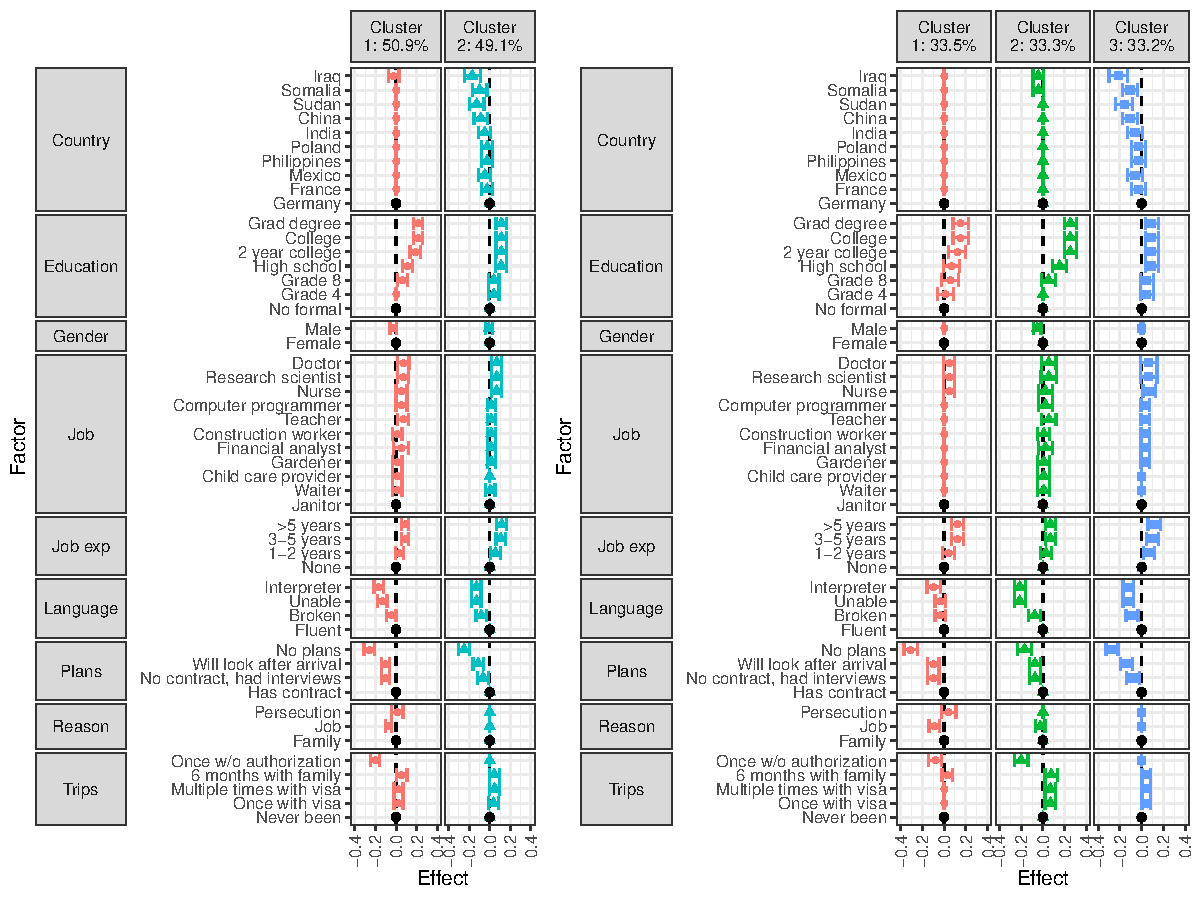
\includegraphics[width=\textwidth]{figures/AME_plot.pdf}
%6x8
\caption{Estimated average marginal component effects using a
  two-cluster (left) and three-cluster (right) analysis. The point
  estimates and 95\% Bayesian credible intervals are shown. A solid
  circle represents the baseline level of each factor.  Number after
  colon give average posterior predictive probability for each
  cluster.} \label{fig:ame}
\end{figure}


Figure~\ref{fig:ame} presents the estimated AMCEs and their 95\%
Bayesian credible intervals for the two-cluster and three-cluster
analyses in the left and right panels, respectively. Cluster~2 in the
two-cluster analysis and Cluster~3 in the three-cluster analysis
display stronger impacts of country of origin than the other clusters.
The respondents in these clusters give the most preference to
immigrants from Germany and the least preference to immigrants from
Iraq (followed by Sudan).  The significant negative effects of Iraq in
Cluster~2 of the two-cluster analysis and Cluster~3 of the
three-cluster analysis are consistent with the significant negative
effect for Iraq found by \cite{hainmueller2015hidden}.  The patterns
we observe for the other factors are also similar for these two
clusters in the two analyses.

Across all clusters, respondents prefer educated and experienced
immigrants who already have contracts (over those who have no
contracts or plans).  Respondents also prefer immigrants who have
better language skills, although this feature matters less for
respondents in Cluster~1 of the three cluster analyses.

For both analyses, the respondents in Cluster~1 do not care much about
immigrant's country of origin.  Instead, they place a greater emphasis
on education and reason for immigration when compared to those in the
other clusters.  For the three-cluster analysis, Clusters~1~and~2
together correspond roughly to Cluster~1 of the two-cluster analysis.
In fact, about 81\% of the respondents who belong to Cluster~1 of the
two-cluster analysis are the members of either Cluster~1~or~2 in the
three-cluster analysis using a weighted average of their estimated cluster membership posterior predictive probabilities.  The differences between Clusters~1~and~2 in
the three-cluster analysis are substantively small, but those in
Cluster~2 appear to place more emphasis on education and prior entry
without legal authorization.  Those in Cluster~1, on the other hand,
give a slight benefit to immigrants whose reason for immigration is
persecution.

It is worth noting that concerns have been raised about comparison of
AMCEs across subgroups as they are inherently dependent on the choice
of baseline \citep{leeper2020measuring}.  As an alternative, we can
compare (and visualize) the marginal means or the values of $\beta$, which have
sum-to-zero constraints, across clusters.
These alternative avoids issues of baseline dependency in comparisons.
A plot of the estimated marginal means is provided in Appendix~\ref{app:emp_marg_means}.
In this case, the results are generally similar to the analysis examined here using AMCEs.


\begin{figure}[t!]
\centering \spacingset{1}
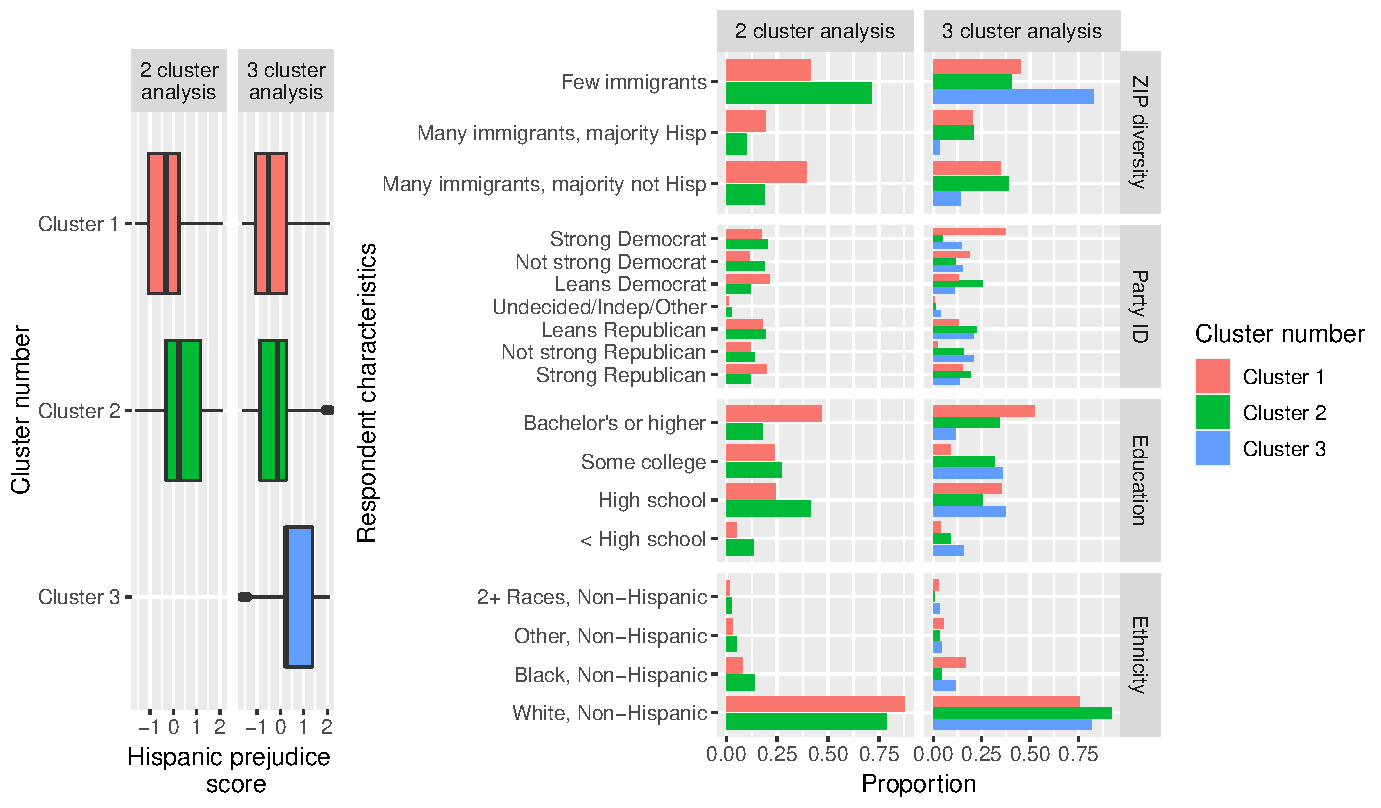
\includegraphics[width=\textwidth]{figures/mod_plot2.pdf}
%9.21x5.39 portrait
\caption{Distribution of respondent characteristics for each cluster.
  Left set of plots shows weighted box plots of the Hispanic prejudice
  moderator within each cluster over the posterior predictive
  distribution using a two-cluster (left) and three-cluster (right)
  analysis.  Right set of plots shows the distribution of categorical
  moderators within each cluster over the posterior predictive
  distribution using a two-cluster (left) and three-cluster (right)
  analysis.  } \label{fig:mod2}
\end{figure}

%\begin{figure}[t!]
%\centering  \spacingset{1}
%\begin{subfigure}[b]{1\textwidth}
%\centering 
%\includegraphics[scale=0.6]{figures/cont_mod_plot.pdf}
%\caption{Weighted box plot showing distribution of the Hispanic prejudice
%  moderator within each cluster over the posterior predictive
%  distribution and survey weight distribution using a two-cluster
%  (left) and three-cluster (right) analysis.}
%     \end{subfigure}
%     \begin{subfigure}[b]{1\textwidth}
%\centering 
%\includegraphics[scale=0.6]{figures/col_bar_mod_plot.pdf}
%\caption{Distribution of categorical moderators within each cluster
%  over the posterior predictive distribution and survey weight
%  distribution using a two-cluster (left) and three-cluster (right)
%  analysis.}
%     \end{subfigure}
%\caption{Distribution of respondent characteristics for each cluster. } \label{fig:mod2}
%\end{figure}

Who belongs to each cluster? One advantage of our method is that it yields a mapping of the moderators to cluster membership probabilities. This allows researchers to interpret cluster membership easily.
%The top panel of Figure~\ref{fig:mod2} shows the distribution of Hispanic prejudice score for each cluster weighted by the corresponding posterior cluster membership probability for each individual respondent.
The left panel of Figure~\ref{fig:mod2} shows the distribution of
Hispanic prejudice score for each cluster weighted by the
corresponding posterior predictive cluster membership probability for each
individual respondent.  The plot shows that for the two-cluster
analysis, those with high prejudice score are much more likely to be
part of Cluster~2. For the three-cluster analyses, those with high
prejudice are more likely to be in Cluster~3. This is consistent with
the finding above that the respondents in those clusters put more
emphasis on immigrant's country of origin.
%The bottom panel of the figure shows the distribution of other respondent characteristics.

The right panel of the figure shows the distribution of other
respondent characteristics.  In general, Cluster~2 in the two-cluster
analysis and Cluster~3 in the three-cluster analysis consist of those
who live in ZIP codes with few immigrants and have lower educational
achievements.  For the three-cluster analysis, those in Cluster~2 tend
to be Republican, where-as those in Cluster~1 are more likely
Democrats.  This is consistent with the finding of a larger penalty
for entry without legal authorization in Cluster~2 of the
three-cluster analysis.  Cluster 3 contains a mix of political
ideologies, though with somewhat more respondents who identify as
Undecided/Independent/Other or not strong Republican than the other
two clusters.

What respondent characteristics are predictive of the cluster membership? 
In addition to the covariate distribution for each cluster shown in
Figure~\ref{fig:mod2}, we can also find how important each moderator is in predicting cluster membership, conditional on all other moderators.
We examine how the predicted probabilities of cluster
memberships change across respondents with different characteristics.
Specifically, we estimate
\begin{equation}
\label{eq:mfx_moderator}
\mathbb{E}\left[\pi_k(X_{ij} = x_1, \bm{X}_{i,-j}) - \pi_{k}(X_{ij} =
  x_0, \bm{X}_{i,-j})\right]
\end{equation}
where $x_0$ and $x_1$ are different values of covariate of interest
$X_{ij}$.  If $X_{ij}$ is a categorical variable, we set $x_0$ to the
baseline level and $x_1$ to the level indicated on the vertical axis.
If $X_{ij}$ is a continuous variable as in the case of the Hispanic
prejudice score, then $x_0$ and $x_1$ represent the 25th and 75th
percentile values.  The solid arrows represent whether the
corresponding 95\% Bayesian credible interval covers zero or not.


\begin{figure}[!t]
\centering \spacingset{1}
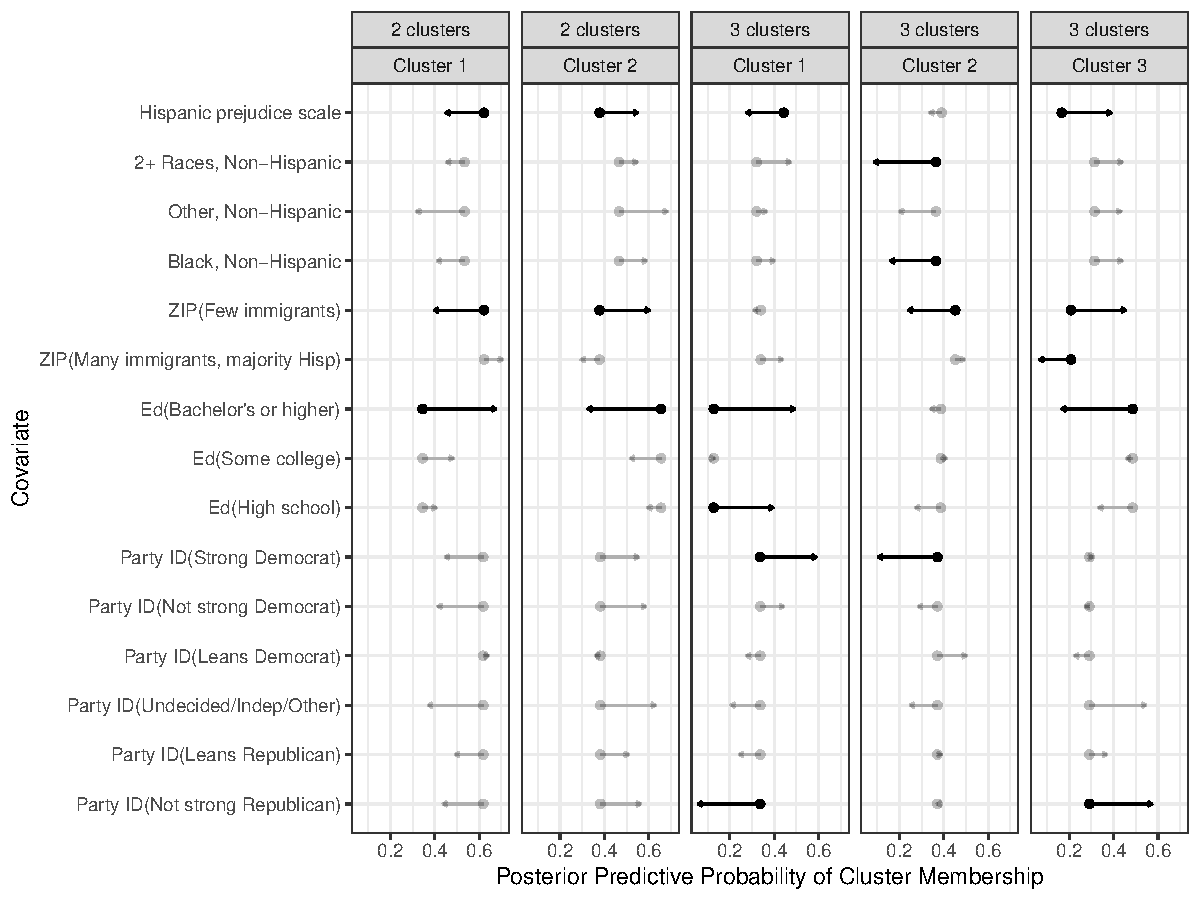
\includegraphics[width=\textwidth]{figures/mod_plot.pdf}
%6x8
\caption{The impact of moderator values on likelihood of being
  assigned to clusters, for two-cluster (left two plots) and
  three-cluster (right three plots) analysis. 
 Dark arrows indicate that there is a significant effect of the moderator on cluster membership, i.e. that the corresponding quantity defined in Equation~\eqref{eq:mfx_moderator} is statistically significant.} \label{fig:mod}
\end{figure}

Consistent with the earlier findings, Figure~\ref{fig:mod} shows that
those with high Hispanic prejudice scores are predicted to belong to
Cluster~2 in the two-cluster analysis and Cluster~3 in the
three-cluster analysis even after controlling for other factors.
These respondents are also less likely to belong to Cluster~1 in
either analysis.  For the three-cluster analysis, party ID appears to
play a statistically significant role (indicated by dark arrow) with
Republicans tending to belong to Cluster~2~or~3 and Democrats tending
to belong to Cluster~1.  Respondents in Cluster~1 tend to have higher
education in both analyses.

Finally, we estimate the average marginal interaction effects (AMIE)
between two factors \citep{egam:imai:19}, which can be computed by
subtracting the two AMCEs from the average effect of changing the two
factors of interest at the same time.  Thus, the AMIE represents the
additional effect of changing the two factors beyond the sum of the
average effects of changing one of the factors alone.  Formally, we
can define the AMIE of changing factors $j$ and $j'$ from levels $l_j$
and $l_{j'}$ to levels $l_j^\prime$ and $l_{j'}^\prime$, respectively,
as follows, 
\begin{equation*}
  \E\{Y_i(T_{ij} = l_j, T_{ij'} = l_{j'}, \bT_{i,-j,-j'}) - Y_i(T_{ij}
  = l_j^\prime, T_{ij'} = l_{j'}^\prime, \bT_{i,-j,-j'})\} -
  \delta_j(l_j, l_j^\prime) - \delta_{j'}(l_{j'}, l_{j'}^\prime).
\end{equation*}

All of the AMIE effects found are quite small, so we do not include
those results here.  According to the skill-premium theory of
\cite{newman2019economic}, we expect to find an interaction between
job and country or education in country, in at least some clusters.
Unfortunately, our analysis does not find support for this hypothesis.


%\begin{figure}[t!]
%\centering  \spacingset{1}
%\includegraphics[width=\textwidth]{figures/AMIE_job_country.pdf}
%%9.21x5.39 portrait
%\caption{Estimated average marginal interaction effects (AMIEs) for
%  the two-cluster (right) and three cluster (left) analysis between
%  country and job.  The interaction effects are detected only for
%  Cluster~1 of both analyses, but their magnitude is
%  small.}\label{fig:amie}
%\end{figure}
%
%As shown in Figure~\ref{fig:amie}, we find interaction effects between
%country and job for Cluster~1 in both analyses.  The effect sizes are
%quite small, but the estimated effects are consistent with the skill
%premium hypothesis of \cite{newman2019economic}.  In particular, it
%appears that individuals who hold higher prejudice (those in
%Cluster~1), do enforce a skill premium for individuals from Iraq in
%terms of job, slightly preferring Iraqi immigrants with high skilled
%jobs, whereas immigrants from Germany show lower preference for
%high-skilled jobs such as doctor.  Interactions among other factors
%were found to be even smaller in magnitude, and therefore are not
%displayed.

\section{Concluding Remarks}\label{sec:disc}

We have shown that a Bayesian mixture of regularized logistic
regressions can be effectively used to estimate heterogeneous
treatment effects of high-dimensional treatments.  The proposed
approach yields interpretable results, illuminating how different sets
of treatments have heterogeneous impacts on distinct groups of units.
We apply our methodology to conjoint analysis, which is a popular
survey experiment in marketing research and social sciences.  Our
analysis shows that individuals with high prejudice score tend to
discriminate against immigrants from certain non-European countries.
These individuals tend to be less educated and live in areas with few
immigrants.  Future research should consider the derivation of optimal
treatment rules in this setting as well as the empirical evaluation of
such rules.  Another important research agenda is the estimation of
heterogeneous effects of high-dimensional treatments in observational
studies.

\bigskip
\bibliographystyle{pa}
\bibliography{het_ref,my,imai}

\newpage
% Manually specify geometry
\begin{appendices}
	\begin{set11}
		\setlength\paperwidth{614.295pt}
		\setlength\paperheight{794.96999pt}
		\setlength\textwidth{469.75502pt}
		\setlength\textheight{650.43001pt}
		\setlength\oddsidemargin{0.0pt}
		\setlength\evensidemargin{0.0pt}
		\setlength\topmargin{-37.0pt}
		\setlength\headheight{12.0pt}
		\setlength\headsep{25.0pt}
		\setlength\topskip{11.0pt}
		\setlength\footskip{30.0pt}
		\setlength\marginparwidth{59.0pt}
		\setlength\marginparsep{10.0pt}
		\setlength\columnsep{10.0pt}
		%\setlength\skip\footins{10.0pt plus 4.0pt minus 2.0pt}
		\setlength\hoffset{0.0pt}
		\setlength\voffset{0.0pt}
		\setlength\mag{1000}
		
		\def\spacingset#1{\renewcommand{\baselinestretch}%
			{#1}\small\normalsize} \spacingset{1}
		\renewcommand\appendixname{Supplementary Material}
		
\def\spacingset#1{\renewcommand{\baselinestretch}%
	{#1}\small\normalsize} \spacingset{1}

\appendix
\setcounter{page}{1}
\begin{center}
{\bf \Large  Supplementary Material for\\``Estimating Heterogeneous Causal Effects of
  High-Dimensional Treatments:  Application to Conjoint Analysis''}

\vspace{0.5cm}
{ \large Max Goplerud \hspace{.5in} Kosuke Imai \hspace{.5in} Nicole E. Pashley}
\end{center}

\setcounter{equation}{0}
\setcounter{figure}{0}
\setcounter{theorem}{0}
\setcounter{lemma}{0}
\setcounter{section}{0}
\setcounter{table}{0}
\renewcommand {\theequation} {A\arabic{equation}}
\renewcommand {\thefigure} {A\arabic{figure}}
\renewcommand {\thealgorithm} {A\arabic{algorithm}}
\renewcommand {\thetable} {A\arabic{table}}
\medskip 

\section{The Details of the Immigration Conjoint Experiment}
\label{app:conjoint}

 \begin{table}[ht!]
    \centering\small
    \begin{tabular}{|p{0.25\linewidth}|p{0.12\linewidth}| p{0.58\linewidth}|}
    \hline
    Attribute &\# of Levels & Levels\\
     \hline
    Education & 7 & No formal education; Equivalent to completing fourth grade in the U.S.; Equivalent to completing eighth grade in the U.S.; Equivalent to completing high school in the U.S.; Equivalent to completing two years at college in the U.S.; Equivalent to completing a college degree in the U.S.; Equivalent to completing a graduate degree in the U.S.\\
    Gender & 2 & Female; Male\\
    Country of origin & 10 & Germany; France; Mexico; Philippines; Poland; India; China; Sudan; Somalia; Iraq\\
    Language & 4 & During admission interview, this applicant spoke fluent English; During admission interview, this applicant spoke broken English; During admission interview, this applicant tried to speak English but was unable; During admission interview, this applicant spoke through an interpreter\\
    Reason for Application & 3 &  Reunite with family members already in U.S.; Seek better job in U.S.; Escape political/religious persecution\\
    Profession & 11 & Gardener; Waiter; Nurse; Teacher; Child care provider; Janitor; Construction worker; Financial analyst; Research scientist; Doctor; Computer programmer\\
    Job experience & 4 & No job training or prior experience; One to two years; Three to five years\\
    Employment Plans & 4 & Has a contract with a U.S. employer; Does not have a contract with a U.S. employer, but has done job interviews; Will look for work after arriving in the U.S.; Has no plans to look for work at this time\\
    Prior Trips to the U.S. & 5 & Never been to the U.S.; Entered the U.S. once before on a tourist visa; Entered the U.S. once before without legal authorization; Has visited the U.S. many times before on tourist visas; Spent six months with family members in the U.S.\\
    \hline
    \end{tabular}\caption{Table 1 in \cite{hainmueller2015hidden}. All attributes for immigrants and their levels.}\label{tab:attributes}
\end{table}

\section{Propriety of the Structured Sparse Prior}
\label{sec:app_ssparse_prior}

The proof of propriety for the structured sparse prior used in our
paper is an application of Theorem~1 established in
\cite{goplerud2021sparsity} and is reproduced here.
\begin{theorem}[\cite{goplerud2021sparsity}] 
	\label{result:goplerud_1}
        Consider the following structured sparse prior on
        $\bm{\beta} \in \mathbb{R}^p$ with regularization strength
        $\lambda > 0$ penalizes $K$ linear constraints $\bm{d}_k$ and
        $L$ quadratic constraints $\bm{F}_\ell$ on the parameters
        where $\bm{F}_\ell$ is symmetric and positive
        semi-definite. The kernel of the prior is shown below.
  $$p(\bm{\beta}) \propto \exp\left(-\lambda \left[\sum_{k=1}^K
      |\bm{d}_k^\top \bm{\beta}| + \sum_{\ell=1}^L \sqrt{
        \bm{\beta}^\top \bm{F}_{\ell} \bm{\beta}}\right] \right)$$ Further
  define $\bm{D}^\top = [d_1, \cdots, d_K]^\top$ and
  $\bar{\bm{D}}^\top = [\bm{D}^\top, \bm{F}_1, \cdots, \bm{F}_L]$.
  Then, for $\lambda >0 $, the prior above is proper if and only if
  $\bar{\bm{D}}$ is full column rank.
\end{theorem}
In our specific case, we note that $K = 0$, $L = G$, and
$\lambda = \lambda \bar{\pi}_k^\gamma$. Prior propriety of
$p(\bm{\beta}_k \mid \{\bm{\phi}_k\}_{k=2}^K, \lambda)$, therefore,
can be determined by empirically investigating whether $\bar{\bm{D}}$,
i.e. the vertically stacked $\bm{F}_\ell$, is full column rank.

It is also possible to analytically show the propriety of the prior
distribution in all cases considered in this paper. We focus on the
case of $K = 1$ and arbitrary $\lambda > 0$ as the result follows
automatically for the case in our paper. 
\begin{result}
	\label{thm:proper_prior}
	Assume a structured sparse prior for a factorial or conjoint
        design with $J$ factors each with $L_j$ levels where all
        pairwise interactions are included and levels of each factor
        are encouraged to be fused together (i.e. the model in the
        main text). The kernel of the prior is shown below where
        $\bm{F}_g$ are as defined in the main text. 	
	$$k(\bm{\beta}) = \exp\left(-\lambda \sum_{g=1}^G \sqrt{\bm{\beta}^\top \bm{F}_g \bm{\beta}}\right)$$
	Assume that the linear sum-to-zero constraints
        $\bm{C}^\top \bm{\beta} = \bm{0}$ hold.  Then, the structured
        sparse prior on the unconstrained $\tilde{\bm{\beta}}$ such
        that $\tilde{\bm{\beta}} \in \mathcal{N}(\bm{C}^\top)$ is
        proper. Or, equivalently, the following result holds.
	$$\int_{\bm{\beta}: \bm{C}^\top \bm{\beta} = \bm{0}} k(\bm{\beta}) d\bm{\beta} < \infty.$$
\end{result}
\begin{proof}
  Let $\mathcal{B}_{\bm{C}^\top}$ represent a basis for the
  linear constraints $\bm{C}^\top$. The integral for evaluating
  propriety can be written as,
  \begin{equation*}
\int_{\tilde{\bm{\beta}}} \tilde{k}(\tilde{\bm{\beta}})
d\tilde{\bm{\beta}}\quad \text{where} \quad \tilde{k}(\tilde{\bm{\beta}}) =
\exp\left(-\lambda \sum_{g=1}^G
  \sqrt{\tilde{\bm{\beta}}^\top\mathcal{B}_{\bm{C}^\top}^\top \bm{F}_g
    \mathcal{B}_{\bm{C}^\top} \tilde{\bm{\beta}}}\right). 
\end{equation*}
Note that $\bm{F}_g$ can be expressed as a sum of $N_g$ outer products
of $|\bm{\beta}|$-length vectors of the form
$\bm{l}_i \in \{-1, 0, 1\}$ where $-1$ and $1$ correspond to the two
terms that are fused together and all other elements are $0$, i.e.,
$ \bm{F}_g = \sum_{g'=1}^{N_g} \bm{l}_{g'}\bm{l}_{g'}^\top$. Thus, one
can define a matrix
$\bm{Q}_g^\top = \left[\bm{l}_1, \cdots, \bm{l}_{N_g}\right]$ such
that $\bm{Q}_g^\top \bm{Q}_g = \bm{F}_g$, which allows us to rewrite
% where each row of $\bm{Q}_g$ has exactly one element as `1' and one as `-1' and the rest are zero. $\bm{Q}_g$ is an orientated incidence matrix of a graph $\mathcal{G}_g$ where each node is a coefficient in $\bm{\beta}$. 
$\tilde{k}(\tilde{\bm{\beta}})$ as:
$$\tilde{k}(\tilde{\bm{\beta}}) = \exp\left(-\lambda \sum_{g=1}^G
  \sqrt{\tilde{\bm{\beta}}^\top
    \left[\mathcal{B}_{\bm{C}^\top}\right]^\top \bm{Q}_g^\top \bm{Q}_g
    \mathcal{B}_{\bm{C}^\top} \tilde{\bm{\beta}}}\right).$$

By applying Theorem~\ref{result:goplerud_1} and noting that the
nullspaces of $\bm{A}^T\bm{A}$ and $\bm{A}$ are identical, the
integral of $\tilde{k}(\tilde{\bm{\beta}})$ is finite if and only if
$\bm{Q}\mathcal{B}_{\bm{C}^\top}$ is full column rank, where
$\bm{Q}^\top = [\bm{Q}^\top_1, \cdots, \bm{Q}^\top_G]$.  We
demonstrate this fact in two steps.  First, there exists a permutation
matrix $\bm{P}_{Q}$ such that $\bm{P}_Q \bm{Q} $ has a block diagonal
structure with $J+1$ diagonal blocks. The first $J$ blocks
corresponding to the main terms for each factor $j$ and the last block
corresponds to all interaction terms. The nullspace of each block is
spanned by the vector $\bm{1}$ as the corresponding block of
$\bm{P}_Q\bm{Q}$ is a (transposed) orientated incidence matrix of a
fully connected graph. Thus, the nullspace of $\bm{P}_Q \bm{Q}$, and
hence $\bm{Q}$, is spanned by the $J+1$ columns of a block diagonal
matrix with $\bm{1}$ on each block.  Second, consider the linear
constraints $\bm{C}^\top \bm{\beta} = \bm{0}$.  The only vector to
satisfy this constraint and lie in the nullspace of $\bm{Q}$ must be
$\bm{0}$ as, for each block, the only vector proportional to $\bm{1}$
and satisfying the corresponding sum-to-zero constraints must be
$\bm{0}$. Thus, $\bm{Q}\mathcal{B}_{\bm{C}^\top}$ is full column rank
and the prior is proper.
\end{proof}

\section{Derivations for the Basic Model}
\label{sec:app_derivations}

This section derives a number of results for the basic model. It first
restates the main results concerning the elimination of the linear
constraints $\bC^\top \bm{\beta}_k = \bm{0}$. Then, it derives the
Expectation Maximization algorithm, our measure of degrees of freedom,
and some additional computational improvements used to accelerate
estimation.  In the following, with a slight abuse of notation, we use
$\bm{t}_i$ to denote the corresponding vector of indicators for
whether certain treatments or interactions are present (i.e. stacking
all $I(T_{ij} = 1)$, etc. from Equation~\ref{eq:define_lp}).  In
addition, we use $\psi_{ik}$ to indicate the linear predictor for
observation $i$ and cluster $k$.

\subsection{Removing the Linear Constraints}
\label{sec:app_derivation_LC}

The inference problem in the main text is presented as an optimization
problem subject to linear constraints on the coefficients
$\bm{\beta}_k$. We note that inference is noticeably easier if these
are eliminated via a transformation of the problem to a
lower-dimensional one by noting that $\bm{\beta}_k$ must lie in the
null space of the constraint matrix $\bm{C}^\top$. Define
$\tilde{\bm{\beta}}_k = \left(\mathcal{B}_{\bC^\top}^\top
  \mathcal{B}_{\bC^\top}\right)^{-1}
\mathcal{B}_{\bC^\top}^\top\bbeta_k$ where $\mathcal{B}_{\bC^\top}$ is
a basis for the null space of $\bC^\top$. Given this, the problem can
be solved in terms of the unconstrained
$\tilde{\bm{\beta}}_k \in \mathbb{R}^{p-\mathrm{rank}(\bC^\top)}$. The
treatment design vectors
($\tilde{\bm{t}}_i = \mathcal{B}_{\bC^\top} \bm{t}_i$) and penalty
matrices ($\tilde{\bF}_g$ as
$\mathcal{B}_{\bC^\top}^\top \bF_g \mathcal{B}_{\bC^\top}$) are
adjusted and then the augmented problem can be written in
Equations~\eqref{eq:augmented1}~and~\eqref{eq:augmented2}. The new
linear predictor is
$\psi_{i,k} = \left[\tilde{\bm{t}}_i\right]^\top
\tilde{\bm{\beta}}_{Z_i} + \mu$.

Note that the only difference between the unconstrained and
constrained problem is the choice of treatment design matrix. Given
this similarity and to reduce the burden of notation, we thus present
all results herein dropping the ``tilde'' notation and note that, once
estimated, $\tilde{\bm{\beta}}_k$ is projected back into the original
space for the reported coefficients, average marginal component effects,
etc. Given Appendix~\ref{sec:app_uncertainty}'s results on
approximating $\tilde{\bm{\beta}}_k$ as normal, $\bm{\beta}_k$ will
have a (singular) normal distribution distribution.

\subsection{Expectation Maximization Algorithm}
\label{sec:app_derivation_EM}

Assume that we have the model after the linear constraints have been removed as discussed above. We begin with the cycle of the AECM algorithm for updating $\{\bm{\beta}_k\}_{k=1}^K$ given $\{\bm{\phi}_{k=2}^K\}$.  The model with triple augmentation is shown below, mirroring Equation~\eqref{eq:aecm_ebeta} from the main text.
\begin{subequations}
	\label{app_eq:augmented}
	\begin{alignat}{2}
	&p(Y_i, \omega_{i} \mid Z_i) = \frac{1}{2} \exp\left[\left(Y_i - \frac{1}{2}\right)
          \psi_{i, Z_i} - \frac{\omega_{i}}{2} \psi_{i, Z_i}^2\right]
        f_{PG}(\omega_{i} \mid 1, 0) \\ 
	&p(\bm{\beta}_k, \{\tau^2_{gk}\} \mid \lambda, \{\bm{\phi}_k\}) \propto \exp\left[-\frac{1}{2}{\bm{\beta}}_k^\top\left(\sum_{g=1}^K \frac{{\bm{F}}_{g}}{\tau^2_{gk}}\right) {\bm{\beta}}_k\right] \cdot \prod_{g=1}^G \frac{\exp\left(-\left[\lambda \bar{\pi}_k\right]^2/2 \cdot \tau^2_{gk}\right)}{\sqrt{\tau^2_{gk}}} \\
	&Z_i \sim \mathrm{Multinomial}\left(1, \bm{\pi}_i\right); \quad \psi_{ik} = \bm{t}_i^\top \bm{\beta}_k + \mu
	\end{alignat}
\end{subequations}

We treat $\{\omega_i, Z_i\}_{i=1}^N$ and $\{\tau^2_{gk}\}$ as missing
data to be used in the $E$-Step and $\bm{\beta}_k$ as parameters to be
optimized in an $M$-Step. For this cycle of the AECM algorithm, we hold $\bm{\phi}$ constant. The $E$-Step can be computed by noting that $p(\omega_i, Z_i \mid Y_i, \bm{\theta})$ and $p(\tau^2_{gk} \mid \bm{\theta})$ are conditionally independent across $i$ and $gk$. The distributions are shown below,
\begin{subequations}
\begin{align}
p(\tau^{-2}_{gk} \mid \bm{\theta}) &\sim \mathrm{InverseGaussian}\left(\frac{\lambda}{\sqrt{\bm{\beta}_k^\top\bm{F}_g\bm{\beta}_k}}, \quad \lambda^2\right), \\
p(Z_i = k \mid Y_i, \bm{\theta}) &\propto p_{ik}^{Y_i} (1-p_{ik})^{1-Y_i} \pi_{ik}; \quad p_{ik} = \frac{\exp(\psi_{ik})}{1+\exp(\psi_{ik})}, \\
p(\omega_i \mid Z_i = k, \bm{\theta}) &\sim \mathrm{PG}\left(1, \psi_{ik}\right).
\end{align}
\end{subequations}
The relevant expectations are shown below,
\begin{subequations}
\begin{align}
& \E\left(\tau^{-2}_{gk}\right) = \frac{\lambda}{\sqrt{\bm{\beta}_k^\top\bm{F}_g\bm{\beta}_k}}; \\
& \E (z_{ik}) = \E\left[I(Z_i = k)\right] = \frac{p_{ik}^{Y_i} (1-p_{ik})^{1-Y_i} \pi_{ik}}{\sum_{\ell=1}^K p_{i\ell}^{Y_i} (1-p_{i\ell})^{1-Y_i} \pi_{i\ell}} \\
& \E (\omega_{i} \mid Z_i = k) = \frac{1}{2\psi_{ik}} \tanh\left(\frac{\psi_{ik}}{2}\right)
\end{align}
\end{subequations}

Note that as $\bm{\beta}_k^\top \bm{F}_g \bm{\beta}_k$ approaches
zero, $\E(\tau^{-2}_{gk})$ approaches infinity. To prevent numerical
instability, we rely on the strategy in \cite{goplerud2021sparsity}
(inspired by \citealt{polson2011svm}) where once it is sufficiently
small, e.g. below $10^{-4}$, and thus the restriction is almost
binding, we ensure that restriction holds in all future iterations. We
do so by adding a quadratic constraint
$\bm{\beta}_k^\top \bm{F}_g \bm{\beta}_k = 0$. Note that this again
implies that $\bm{\beta}_k$ lies in the nullspace of $\bm{F}_g$ and
thus with an additional transformation, it can be removed and the
problem be solved in an unconstrained space with a modified design.

With these results, the $Q_\beta$-function can be thus expressed as the
expectation of the logarithm of the augmented posterior where we suppress all terms
that do not depend on $\bm{\beta}_k$ and all expectations depend on prior value $\bm{\theta}^{(t)}$. Recall that $\bm{\beta} = \{\{\bm{\beta}_k\}_{k=1}^K, \mu\}$.

\begin{align}
  & Q_\beta\left(\bm{\beta}, \bm{\theta}^{(t)}\right)\nonumber  \\
  = &\sum_{i=1}^N \left[\sum_{k=1}^K \E(z_{ik})\left\{\left(Y_i -
      \frac{1}{2}\right) \psi_{ik} - \E(\omega_i \mid Z_i = k)
      \frac{\psi^2_{ik}}{2}\right\} \right]  + \sum_{k=1}^K -\frac{1}{2}
      \bm{\beta}_k^\top \left[\sum_{g=1}^K \bm{F}_g \cdot
     \E(1/\tau^2_{gk})\right] \bm{\beta}_k + \text{const.} \label{eq:q_func}
\end{align}

From the above, define a vector that concatenates
$\check{\bm{\beta}}^\top = [\mu, \bm{\beta}_1, \cdots,
\bm{\beta}_K]^\top$. We can create a corresponding design
$\check{\bm{T}} = [\bm{1}_{N}, \bm{I}_K \otimes \bm{T}]$
where $\bm{T}^\top = [\bm{t}_1, \cdots, \bm{t}_N]$. We further create
a corresponding diagonal weight matrix
$\check{\bm{\Omega}} =
\mathrm{diag}\left(\{\{\E(z_{ik})\E(\omega_{i}\mid Z_i =
  k)\}_{i=1}^N\}_{k=1}^K\right)$. Further, we can create the combined
ridge penalty
$\bm{\mathcal{R}} = \mathrm{blockdiag}\left(\{0,
  \{\bm{R}_k\}_{k=1}^K\}\right)$ where
$\bm{R}_k = \sum_g \bm{F}_g \E(\tau^{-2}_{gk})$. Finally, we can
create the augmented outcome
$\check{\bm{Y}} = \{\{\E(z_{ik}) (Y_i - 1/2)\}_{i=1}^N\}_{k=1}^K$. With
this in hand, we can rewrite the $Q_\beta$ function as proportional to
the following ridge regression problem and the corresponding update in
the $M$-Step.
\begin{align*}
  Q_\beta\left(\bm{\beta};
  \bm{\theta}^{(t)}\right) & = \check{\bm{Y}}^\top
                               \left(\check{\bm{T}}
                               \check{\bm{\beta}}\right) - \frac{1}{2}
                               \check{\bm{\beta}}^\top
                               \check{\bm{T}}^\top \check{\bm{\Omega}}
                               \check{\bm{T}} \check{\bm{\beta}} -
                               \frac{1}{2} \check{\bm{\beta}}^\top
                               \bm{\mathcal{R}} \check{\bm{\beta}}  + \text{const.},\\
  \check{\bm{\beta}}^{(t+1)} &= \left(\check{\bm{T}}^\top \check{\bm{\Omega}} \check{\bm{T}} + \bm{\mathcal{R}}\right)^{-1} \check{\bm{T}}^\top \check{\bm{Y}}.
\end{align*}
Note that since $\check{\bm{\Omega}}$, $\check{\bm{Y}}$, and
$\mathcal{\mathbb{R}}$ depend on $\bm{\theta}^{(t)}$, we can think
about this algorithm as follows where we denote their dependence on
prior values with the superscript $(t)$.
$$\check{\bm{\beta}}^{(t+1)}  = \left(\check{\bm{T}}^\top \check{\bm{\Omega}}^{(t)} \check{\bm{T}} + \bm{\mathcal{R}}^{(t)}\right)^{-1} \check{\bm{T}}^\top \check{\bm{Y}}^{(t)} $$

In practice, we rely on a generalized EM algorithm where $Q_\beta$ is
improved versus maximized for computational reasons; we do so using a
conjugate gradient solver initialized at
$\check{\bm{\beta}}^{(t)}$. The update for $\{\bm{\phi}_k\}_{k=2}^K$
is shown in the main text; as is required for AECM algorithms, it requires a re-computation of the $E$-Step for $\E(z_{ik})$ that depends on $\bm{\beta}^{(t+1)}$. We use L-BFGS-B for a few steps to improve the objective.

\subsection{Degrees of Freedom}
\label{sec:app_derivations_df}

We note that our procedure for estimating $\check{\bm{\beta}}^{(t)}$
appears similar to the results in \cite{oelker2017uniform} where
complex regularization and non-linear models can be recast as a
(weighted) ridge regression. Using that logic, we take the trace of
the ``hat matrix'' implied by our algorithm at stationarity to
estimate our degrees of freedom. We also adjust upwards the degrees of
freedom by the number of moderator coefficients (e.g.,
\citealt{khalili2010mixture,chamroukhi2019regularized}).

Equation~\eqref{eq:df} shows our procedure where $\bm{\mathcal{R}}$
and $\check{\bm{\Omega}}$ contain expectations calculated at
convergence. $p_x$ denotes the number of moderators, i.e. the
dimensionality of $\bm{\phi}_k$. Before evaluating
Equation~\eqref{eq:df}, for any two factor levels that are
sufficiently close (e.g.,
$\sqrt{\bbeta_k^\top\bF_g \bbeta_k} < 10^{-4}$), we assume they are
fused together and consider it as an additional linear constraint on
the parameter vector $\bm{\beta}_k$.

\begin{equation}
\label{eq:df}
\begin{split}
&\mathrm{df} = \mathrm{tr}\left[\left(\check{\bm{T}}^\top \check{\bm{\Omega}} \check{\bm{T}} + \bm{\mathcal{R}}\right)^{-1} \check{\bm{T}}^\top \check{\bm{\Omega}} \check{\bm{T}}\right] + p_x \left(K - 1\right)
\end{split}
\end{equation}

From this, we can calculate a BIC criterion. We seek to find the
regularization parameter $\lambda$ that minimizes this criterion. To
avoid the problems of a naive grid-search, we use Bayesian model-based
optimization that attempts to minimize the number of function
evaluations while searching for the value of $\lambda$ that minimizes
the BIC (\texttt{mlrMBO}; \citealt{bischl2018mlrmbo}). We find that
with around fifteen model evaluations, the optimizer can usually find
a near optimal value of $\lambda$.

\subsection{Computational Improvements}
\label{sec:app_derivations_improve}

While the algorithm above provides a valid way to locate a posterior
mode, our estimation problem is complex and
high-dimensional. Furthermore, given the complex posterior implied by
mixture of experts models, we derived a number of computational
strategies to improve convergence. We use the SQUAREM algorithm
(\citealt{varadhan2008simple}) and a generalized EM algorithm to
update $\bm{\beta}$ using a conjugate gradient approach and
$\bm{\phi}$ using a few steps of L-BFGS-B.

We also outline a way to deterministically initialize the model to provide stability and, again, speed up estimation on large problems. To do this, we adapt the procedure from \cite{murphy2020init} for initializing mixture of experts: (i) initialize the clusters using some (deterministic) procedure (e.g. spectral clustering on the moderators); (ii) using only the main effects, estimate an EM algorithm---possibly with hard assignment at the $E$-Step (CEM; \citealt{celeux1992classification}); (iii) iterate until the memberships have stabilized. Use those memberships to initialize the model. This has the benefit of having a deterministic initialization procedure where the cluster members are based on the moderators but guided by which grouping seem to have sensible treatment effects, at least for the main effects. Given the memberships, update $\bm{\beta}$ using a ridge regression and $\bm{\phi}$ using a ridge regression and take those values as $\bm{\beta}^{(0)}$ and $\bm{\phi}^{(0)}$.



\section{Extensions to the Basic Model}
\label{sec:app_extensions}

As noted in the main text, there are five major extensions to the basic model that applied users might wish to include:

\begin{enumerate}
	\item Repeated tasks (observations) for a single individual
	\item A forced-choice conjoint experiment
	\item Survey  to weight the sample estimate to the broader population
	\item Adaptive weights for each penalty
	\item Latent overlapping groups
\end{enumerate}

All can be easily incorporated into the proposed framework above. This
section outlines the changes to the underlying model.

\subsection{Repeated Observations}
\label{sec:app_extensions_repeat}

This modification notes that in factorial and conjoint experiments it
is common for individuals to perform multiple tasks. Typically, the
number of tasks $N_i$ is similar across individuals. The updated
likelihood for a single observation $i$ is shown below; we show both
the observed and complete case. $y_{it}$ represents the choice of
person $i$ on task $t \in \{1, \cdots, N_i\}$; $p_{itk}$ is the
probability of $Y_{it} = 1$ if person $i$ was in cluster $k$. 
\begin{align}
  &L\left(\{Y_{it}\}_{t=1}^{N_i}\right) = \sum_{k=1}^K \pi_{ik} \left[\prod_{t=1}^{N_i} p_{itk}^{Y_{it}} (1-p_{itk})^{1-Y_{it}} \right]; \quad p_{itk} = \frac{\exp(\psi_{itk})}{1+\exp(\psi_{itk})}; \quad \psi_{itk} = \bm{t}_{it}^\top\bm{\beta}_k + \mu 
\label{app_eq:repeated} \\
  &L^c(\{y_{it}, \omega_{it}\} \mid Z_i) = \prod_{t=1}^{N_i}
    \left[\frac{1}{2} \exp\left\{\left(Y_{it} - \frac{1}{2}\right)
    \psi_{i, Z_i} - \omega_{it} \frac{\psi_{it,Z_i}^2}{2}\right\}
    f_{PG}(\omega_{it} \mid 1, 0) \right]  
\end{align}

Note that because of the conditional independence of
$(y_{it}, \omega_{it})$ given $Z_i$ and the parameters, the major
modifications to the EM algorithm is that the $E$-Step must account
for all $t$ observations, i.e. the terms summed in
Equation~\eqref{app_eq:repeated}. Some additional book-keeping is
required in the code as the design of the treatments has
$\sum_{i=1}^N N_i$ rows whereas the design of the moderators has $N$
rows. Repeated observations can be easily integrated into the
uncertainty estimation procedure outlined below.

\subsection{Forced Choice Conjoint Design}
\label{sec:app_extensions_forced}

A popular design of a conjoint experiment is the forced choice design
where the respondents are required to choose between two profiles.
Therefore, the researcher does not observe an outcome for each profile
separately, but rather a single outcome is observed for each pair
indicating which is preferred. \cite{egam:imai:19} show that this can
be easily fit into the above framework with some adjustment.
Specifically, the model is modified to difference the indicators of
the treatment levels for the pair of profiles (subtracting, e.g., the
levels of the profile presented on the left from those of the profile
presented on the right). The intercept for this model can be
interpreted as a preference for picking a profile presented in a
particular location.  With this modification, estimation proceeds as
before.

\subsection{Standardization Weights}
\label{sec:app_extensions_standardization}

An additional modification to the problem is to weight the
penalty. This could be done for two reasons.  First, there is an issue
of the columns having different variances/Euclidean norms because of
the different number of factor levels $L_j$. Second, it is popular to
weight the penalty based on some consistent estimator (e.g. ridge
regression) to improve performance and, in simpler models, can be
shown to imply various oracle properties
(e.g. \citealt{zou2006adaptive}). We leave the latter to future
exploration.

Define $\xi_{gk}$ as a positive weight for the $g$-th penalty and the
$k$-th cluster. The kernel of the penalty is modified to include
them. 
\begin{equation}
\ln p(\bm{\beta}_k \mid \lambda, \gamma, \{\bm{\phi}_k\}) \propto -\lambda \bar{\pi}_k^\gamma \sum_{g=1}^G \xi_{gk} \sqrt{\bm{\beta}_k^\top \bm{F}_g \bm{\beta}_k}
\end{equation}
This has no implication on the rank of the stacked $\bm{F}_g$ (and
thus the results in Appendix~\ref{sec:app_ssparse_prior}) as they are
all positive and thus only slightly modify the $E$-Step. 

We employ weights in all of our analyses to account for the fact that
different factors $j$ may have different number of levels $L_j$. We
use a generalization of the weights in \cite{bondell2009anova} to the
case of penalized \emph{differences}. Specifically, consider the
over-parameterized model in Appendix~\ref{sec:app_log} where the
penalty can be written entirely on the differences
$\bm{\delta}_{\mathrm{Main}}$, $\bm{\delta}_{\mathrm{Int}}$,
$\bm{\delta}_{\mathrm{Main-Copy}}$.  Note that each of those penalties
has a simple (group) LASSO form and thus we adopt the approach in
\cite{lim2015learning} of weighting by the Frobenius norm of the
associated columns in $\bm{T}_{\mathrm{LOG}}$, i.e. the
over-parameterized design matrix. At slight abuse of notation, define
$[\bm{T}_{\mathrm{LOG}}]_g$ as the columns of $\bm{T}_{\mathrm{LOG}}$
corresponding to the differences penalized in the (group) lasso $g$,
the weight can be expressed as follows:
$$\xi_{gk} = \frac{1}{\sqrt{N}}||~\left[\bm{T}_{\mathrm{LOG}}\right]_{g} ||_F$$
Ignoring the factor of $\sqrt{N}$, this exactly recovers the weight proposed in \cite{bondell2009anova} in the non-latent-overlapping non-interactive model of $(L_j + 1)^{-1} \sqrt{N^j_{l} + N^j_{l'}}$ where $N^j_l$, $N^j_{l'}$ are the number of observations for factor $j$ in level $l$ and level $l'$ that are being encouraged to fuse together by the penalty in group $g$.



\subsection{Latent Overlapping Groups}
\label{sec:app_log}

One feature of the above approach is that our groups are highly
overlapping. \cite{yan2017hierarchical} suggest that, in this setting,
a different formulation of the problem may result in superior
performance (see also \citealt{lim2015learning}). Existing work on the
topic has focused on group LASSO penalties (e.g. $\bm{F}_g = \bm{I}$)
and thus some modifications are needed for our purposes. To address
this, we note that we can again recast our model in an equivalent
fashion.  Instead of penalizing
$\sqrt{\bm{\beta}_k^\top\bm{F}_g \bm{\beta}_k}$, we can penalize the
vector of differences between levels as long as we also impose linear
constraints to ensure that the original model is maintained.

Consider a simple example with two factors each with two levels
$\{1,2\}$ and $\{A,B\}$.  The relevant differences are defined such
that $\delta^j_{1-2} = \beta^j_{1} - \beta^j_2$ and
$\delta^{jj'}_{(lm) - (l'm')} = \beta^j_{l,m} -
\beta^{j'}_{l',m'}$. The equivalent penalty can be imposed as follows:
\begin{equation}
\begin{split}
&\sqrt{\left(\delta^j_{1-2}\right)^2 + \left(\delta^{jj'}_{(1A) - (2A)}\right)^2 + \left(\delta^{jj'}_{(1B)-(2B)}\right)^2} = \sqrt{\bm{\delta}^\top \bm{\delta}}; \quad \bm{\delta} = \left(\begin{array}{c} \delta^j_{1-2} \\ \delta^{jj'}_{(1A)-(2A)} \\ \delta^{jj'}_{(1B)-(2B)} \end{array}\right) \\
&\mathrm{such~that}~\left[\begin{array}{l} \delta^j_{1-2} \\ \delta^{jj'}_{(1A)-(2A)} \\ \delta^{jj'}_{(1B)-(2B)} \end{array}\right] = \left[\begin{array}{lll} \beta^j_1 - \beta^j_2 \\ \beta^{jj'}_{1A} - \beta^{jj'}_{2A} \\ \beta^{jj'}_{1B} - \beta^{jj'}_{2B} \end{array}\right]
\end{split}
\end{equation} 
The latent overlapping group suggests a slight modification.  In
addition to the above penalization of the $\ell_2$ norm of the main
and interactive differences,\footnote{Note the related ``hierarchical
  group LASSO'' would add separate individual penalties for each of
  the interactions. It is easy to include that in our approach.} it
duplicates the main effect and penalizes it separately while ensuring
that all effects maintain the accounting identities between the
``latent'' groups and the overall effect. Specifically, it modifies
the above penalty to duplicate the column corresponding to
$\delta^j_{1-2}$ and adds a new parameter
$\delta^j_{(1-2)-\mathrm{Copy}}$.

\begin{equation}
\begin{split}
\sqrt{\bm{\delta}^\top\bm{\delta}} + |\delta^j_{(1-2)-\mathrm{Copy}}| \quad \mathrm{such~that}~\left[\begin{array}{l} \delta^j_{1-2} \\ \delta^{jj'}_{(1A)-(2A)} \\ \delta^{jj'}_{(1B)-(2B)} \end{array}\right] + \left[\begin{array}{l} \delta^j_{(1-2)-\mathrm{Copy}} \\ 0 \\ 0 \end{array}\right] = \left[\begin{array}{lll} \beta^j_1 - \beta^j_2 \\ \beta^{jj'}_{1A} - \beta^{jj'}_{2A} \\ \beta^{jj'}_{1B} - \beta^{jj'}_{2B} \end{array}\right]
\end{split}
\end{equation} 

Scoping out to the full problem, define $\bm{\delta}_{\mathrm{Main}}$
as the main effect differences, e.g. $\delta^j_{1-2}$, and
$\bm{\delta}_{\mathrm{Int}}$ as the interaction differences and
$\bm{D}_{\mathrm{Main}}$ as the matrix such that
$\bm{D}_{\mathrm{Main}} \bm{\beta} = \bm{\delta}_{\mathrm{Main}}$, and
$\bm{D}_{\mathrm{Int}}$ as the corresponding matrix to create the
vector of interactions. Define $\bm{\delta}_{\mathrm{Main}-g}$ as the
sub-vector of $\bm{\delta}_{\mathrm{Main}-g}$ that corresponds to the
(main) effect differences between levels $l$ and $l'$ of factor $j$
penalized by $\bm{F}_g$ in the original notation. Similarly define
$\bm{\delta}_{\mathrm{Int}-g}$ and
$\bm{\delta}_{\mathrm{Main-Copy}-g}$.

\begin{equation}
\begin{split} &p(\bm{\beta},\bm{\delta}_{\mathrm{Main}}, \bm{\delta}_{\mathrm{Int}}, \bm{\delta}_{\mathrm{Main-Copy}}) =  \sum_{g=1}^G \sqrt{\bm{\delta}_{\mathrm{Main}-g}^T \bm{\delta}_{\mathrm{Main}-g} +  \bm{\delta}_{\mathrm{Int}-g}^T \bm{\delta}_{\mathrm{Int}-g}} +\sum_{g'=1}^{G} \sqrt{\left[\bm{\delta}_{\mathrm{Main-Copy}-g}\right]^2}\\
  &\mathrm{s.t.} \quad \left[\begin{array}{llll} \bm{C}^\top & \bm{0} & \bm{0} & \bm{0} \\ \bm{D}_{\mathrm{Main}} & -\bm{I} & \bm{0} & -\bm{I} \\ \bm{D}_{\mathrm{Int}} & \bm{0} & -\bm{I} & \bm{0} \end{array}\right] \left[\begin{array}{l} \bm{\beta} \\ \bm{\delta}_{\mathrm{Main}} \\ \bm{\delta}_{\mathrm{Int}} \\ \bm{\delta}_{\mathrm{Main-Copy}} \end{array}\right] = \bm{0} \end{split}
\end{equation} 

This also requires a modification of the design matrix $\bm{T}$ to ensure that (i) its dimensionality conforms with the expanded parameter vector and (ii) that for any choice of the expanded parameter that satisfies the constraints, the linear predictor for all observation (and thus the likelihood) is unchanged. Consider first the simple case without latent-overlapping groups. In this case, following \cite{bondell2009anova}, note that the expanded design can be expressed as $\tilde{\bm{T}} = \bm{T}\tilde{\bm{M}}^\dagger$ where $\tilde{\bm{M}}^\top = [ \bm{I}, \bm{D}_{\mathrm{Main}}^\top, \bm{D}_{\mathrm{Int}}^\top]$ and $\tilde{\bm{M}}^\dagger$ is a left-inverse of $\tilde{\bm{M}}$. The latent-overlapping group formulation is a simple extension; we copy the columns of $\tilde{\bm{T}}$ that correspond to $\bm{\delta}_{\mathrm{Main}}$ and append them to get $\bm{T}_{\mathrm{LOG}}$.

With this new design and parameterization in hand, we can again use the above results on projecting out the linear constraints to turn the problem into inference on an unconstrained vector $\bm{\beta}_k$ with a set of positive semi-definite constraints $\{\bm{F}_g\}_{g=1}^{2G}$ and inference proceeds identically to before.


\section{Estimators}\label{append:amce_acie_der}

Here we provide further details on the estimators.  In particular, we
discuss estimation of Average Marginal Component Effects (AMCEs) and
Average Marginal Interaction Effects (AMIEs) based on our model.  We
consider a traditional factorial design, where each unit receives one
treatment (profile), and a conjoint design in which each unit compares
two treatments (profiles).  We also discuss the impact of
randomization restrictions on estimators and implied changes in
interpretation of estimands.

\subsection{Factorial designs}\label{append:amce_fac}

\subsubsection{Without restrictions on randomization}\label{append:fac_unrest_rand}

For a unit in cluster $k$ we have
\begin{equation}
\Pr(Y_i = 1 \mid \bT_i, \bX_i)  = \zeta_{k}(\bT_i) 
\end{equation}
where $i=1,2,\ldots,N$ and for $k=1,2,\ldots,K$,
\begin{equation}
  \zeta_{k}(\bT_i) \
= \ \frac{\exp(\psi_{k}(\bT_i))}{1+\exp(\psi_{k}(\bT_i))}.
\end{equation}
We model $\psi_{k}(\bT_i)$ as
\begin{equation}
\label{eq:define_lp}
\psi_{k}(\bT_i) \ =\ \mu + \sum_{j=1}^J \sum_{l =0}^{L_j-1} 
\mathbf{1}\{T_{ij} = l\} \beta^j_{kl} + \sum_{j=1}^{J-1} \sum_{j' >
  j} \sum_{l=0}^{L_j-1} \sum_{l' = 0}^{L_{j'}-1} \mathbf{1}\{T_{ij} = l,
T_{ij'} = l'\} \beta^{jj'}_{kll'}, 
\end{equation}
for each $k=1,2,\ldots,K$, with constraints
\begin{equation}
  \bC^\top \bbeta_k \ = \ \bm{0} %\label{eq:constraint}
\end{equation}
where $\bbeta_k$ is a stacked column vector containing all coefficients
for cluster $k$.


We can rewrite this to aid in the interpretation of $\bm{\beta}_k$ as follows:
\begin{align*}
  \text{logit}(\zeta_{k}(\bT_i))= \mu + \sum_{j=1}^J \sum_{l =0}^{L_j-1} 
\mathbf{1}\{T_{ij} = l\} \beta^j_{kl} + \sum_{j=1}^{J-1} \sum_{j' >
  j} \sum_{l=0}^{L_j-1} \sum_{l' = 0}^{L_{j'}-1} \mathbf{1}\{T_{ij} = l,
T_{ij'} = l'\} \beta^{jj'}_{kll'}.
\end{align*}
Thus, $\beta^j_{kl}-\beta^j_{kf}$ is the AMCE going from level $f$ to level $l$ of factor $j$ on the logit probability of $Y_i=1$ scale.
 
 Let $\bm{t}$ be some combination of the $J$ factors, where $\bm{t}_j$ is the $j$th factor's level and $\bm{t}_{-j}$ is the levels for all factors except $j$.
This allows us to easily write, taking expectation over units in cluster $k$,
 \begin{align*}
 \E\left(Y_i\mid Z_i=k, {T}_{ij}=l, \bm{T}_{i,-j} = \bm{t}_{-j}\right)
   &= \Pr\left(Y_i = 1|Z_i=k, \bm{T}_{i,j}=l, \bm{T}_{i,-j} = \bm{t}_{-j}\right)\\
 &= \frac{\exp( \zeta_{k}(T_{ij} = l, \bT_{i,-j} = \bm{t}_{-j}))}{1+\exp(\zeta_{k}(T_{ij} = l, \bT_{i,-j} = \bm{t}_{-j}))},
 \end{align*}
 where $T_{ij} = l$ indicates for unit $i$ forcing factor $j$ to be assigned level $l$ and $\bT_{i,-j} = \bm{t}_{-j}$ indicates forcing the assignment on all factors except for $j$ to be assigned levels as in $\bm{t}_{-j}$.
 
 The causal effects of interest (on the original $Y$ scale) are
 defined as contrasts of these expectations.  Without additional
 weighting (i.e., using traditional uniform weights for
 marginalization), the AMCE for level $l$ vs $f$ of factor $j$ in
 cluster $k$ is,
\begin{align*}
\delta^*_{jk}(l,f)=
&\frac{1}{M}\sum_{\bm{t_{-j}}}\E\left(Y_i \mid  Z_i=k, {T}_{ij}=l,
                      \bm{T}_{i,-j} = \bm{t}_{-j}\right) -
                      \E\left(Y_i\mid Z_i=k, {T}_{ij}=f, \bm{T}_{i,-j} =
                      \bm{t}_{-j}\right) \\ 
= &\frac{1}{M}\sum_{\bm{t_{-j}}} \frac{\exp( \zeta_{k}(T_{ij} = l, \bT_{i,-j} = \bm{t}_{-j}))}{1+\exp(\zeta_{k}(T_{ij} = l, \bT_{i,-j} = \bm{t}_{-j}))} -\frac{\exp( \zeta_{k}(T_{ij} = f, \bT_{i,-j} = \bm{t}_{-j}))}{1+\exp(\zeta_{k}(T_{ij} = f, \bT_{i,-j} = \bm{t}_{-j}))},
\end{align*}
where $M$ is the number of possible combinations of the other $J-1$ factors (e.g., if we had $J$ 2-level factors, $M=2^{J-1}$).
We can estimate this by plugging in the coefficients directly.
Note that, because of the nonlinear nature of the estimator, this approach is consistent (under model assumptions) but not unbiased.
 
Alternatively, instead of summing over all \textit{possible}
$\bm{t}_{-j}$, we can use the empirical distribution of $\bm{t}_{-j}$
in the sample.  This potentially changes the estimand.
% Let $\mathcal{H}_k$ be the set of units that we ``assign'' to cluster $k$ based on their posterior probability and let the size of this group be $|\mathcal{H}_k| = N_k$.
Define estimators
  \begin{align*}
 \widehat{\psi}_{k}(\bm{t}) \ =\ \mu + \sum_{j=1}^J \sum_{l =0}^{L_j-1} 
\mathbf{1}\{t_{j} = l\} \widehat{\beta}^j_{kl} + \sum_{j=1}^{J-1} \sum_{j' >
  j} \sum_{l=0}^{L_j-1} \sum_{l' = 0}^{L_{j'}-1} \mathbf{1}\{t_{j} = l,
t_{j'} = l'\} \widehat{\beta}^{jj'}_{kll'}
 \end{align*}
 and 
\begin{align*}
\widehat{y}_k(\bm{t}) = \frac{\exp(   \widehat{\psi}_{k}(\bm{t}) )}{1+\exp(  \widehat{\psi}_{k}(\bm{t}) )}
\end{align*}
 
 Then we can use the following overall estimator for the AMCE:
  \begin{align*}
%&\frac{1}{N_k}\sum_{b \in \mathcal{H}_k}\left(\hat{y}_k(\bm{t}_j=l,\bm{T}_{b,-j} ) -\hat{y}_k(\bm{t}_j=f,\bm{T}_{b,-j}) \right).
&\frac{1}{N}\sum_{b=1}^{N}\left(\widehat{Y}_k(T_{bj}=l,\bm{T}_{b,-j} ) -\widehat{Y}_k(T_{bj}=f,\bm{T}_{b,-j}) \right).
\end{align*}
 This is a consistent estimator (under model assumptions) of
 \begin{align*}
%&\frac{1}{N_k}\sum_{b \in \mathcal{H}_k}\left(E\left[y_i|Z_i=k, \bm{T}_{i,j}=l, \bm{T}_{i,-j} = \bm{T}_{b,-j}\right] -E\left[y_i|Z_i=k, \bm{T}_{i,j}=f, \bm{T}_{i,-j} = \bm{T}_{b,-j}\right] \right)\\
%&=\frac{1}{N_k}\sum_{b \in \mathcal{H}_k}\left(\frac{\exp( g_k(\bm{t}_j=l,\bm{T}_{b,-j} ))}{1+\exp(g_k(\bm{t}_j=l,\bm{T}_{b,-j} ))} -\frac{\exp( g_k(\bm{t}_j=f,\bm{T}_{b,-j}))}{1+\exp(g_k(\bm{t}_j=f,\bm{T}_{b,-j} ))} \right),
   &\frac{1}{N}\sum_{b=1}^N\E\left(Y_i \mid Z_i=k, \bm{T}_{ij}=l,
     \bm{T}_{i,-j} =  \bm{T}_{b,-j}\right) - \E\left(Y_i\mid
     Z_i=k,  \bm{T}_{ij}=f, \bm{T}_{i,-j} = \bm{T}_{b,-j}\right)\\
   = & \frac{1}{N}\sum_{b =1}^N\frac{\exp( \psi_k(T_{bj}=l,\bm{T}_{b,-j} ))}{1+\exp(\psi_k(T_{bj}=l,\bm{T}_{b,-j} ))} -\frac{\exp( \psi_k(T_{bj}=f,\bm{T}_{b,-j}))}{1+\exp(\psi_k(T_{bj}=f,\bm{T}_{b,-j} ))},
\end{align*}
 conditioning on the treatments we actually observed. 
 
 Now, we turn to examination of the AMIEs.  Without additional
 weighting (i.e., using traditional uniform weights for
 marginalization), the AMIE for level $l$ of factor $j$ and level $q$
 of factor $s$ vs $f$ of factor $j$ and level $r$ of factor $s$ in
 cluster $k$ is
\begin{align*}
\text{AMIE}^*_{jsk}(l,f, q, r) =\text{ACE}^*(l,f, q, r) -\delta^*_{jk}(l,f)-\delta^*_{sk}(q,r)
\end{align*}
where
\begin{align*}
&\text{ACE}^*(l,f, q, r)\\
= &\frac{1}{M^*}\sum_{\bm{t_{-(j,s)}}} \E\left(Y_i \mid Z_i=k,
    T_{ij}=l,  T_{is}=q, \bm{T}_{i,-(j,s)} = \bm{t}_{-(j,s)}\right)
    -\E\left(Y_i\mid Z_i=k, T_{ij}=f,  T_{is}=r, \bm{T}_{i,-(j,s)} =
    \bm{t}_{-(j,s)}\right) \\  
=&\frac{1}{M^*}\sum_{\bm{t_{-(j,s)}}}\frac{\exp( \psi_k(T_{ij}=l,
   T_{is}=q, \bm{T}_{i,-(j,s)}=\bm{t}_{-(j,s)}
   ))}{1+\exp(\psi_k(T_{ij}=l,
   T_{is}=q,\bm{T}_{i,-(j,s)}=\bm{t}_{-(j,s)} ))} -\frac{\exp(
   \psi_k(T_{ij}=f, T_{is}=r,\bm{T}_{i,-(j,s)}=\bm{t}_{-(j,s})
   ))}{1+\exp(\psi_k(T_{ij}=f,
   T_{is}=r,\bm{T}_{i,-(j,s)}=\bm{t}_{-(j,s)} ))}, 
\end{align*}
where $M^*$ is the number of possible combinations of the other $J-2$ factors (e.g., if we had $J$ two-level factors, $M^* = 2^{J-2}$).

We can use the following overall estimator for the ACE:
  \begin{align*}
%\frac{1}{N_k}&\sum_{b \in \mathcal{H}_k}\left(\hat{y}_k(\bm{t}_j=l, \bm{t}_s=q, \bm{T}_{b,-(j,s)} ) -\hat{y}_k(\bm{t}_j=f, \bm{t}_s=q, \bm{T}_{b,-(j,s)}) \right)\\
%&-\sum_{b \in \mathcal{H}_k}\left(\hat{y}_k(\bm{t}_j=l, \bm{t}_s=r, \bm{T}_{b,-(j,s)} ) -\hat{y}_k(\bm{t}_j=f, \bm{t}_s=r, \bm{T}_{b,-(j,s)}) \right).
\widehat{\text{ACE}}^*(l,f, q, r) =\frac{1}{N}&\sum_{b =1}^N \widehat{Y}_k(T_{bj}=l, T_{bs}=q, \bm{T}_{b,-(j,s)} ) -\widehat{Y}_k(T_{bj}=f, T_{bs}=r, \bm{T}_{b,-(j,s)}).
\end{align*}
This is then combined with the estimators for the AMCEs to get
\begin{align*}
\widehat{\text{AMIE}}^*_{jsk}(l,f, q, r) =\widehat{\text{ACE}}^*(l,f, q, r) -\widehat{\delta}^*_{jk}(l,f)-\widehat{\delta}^*_{sk}(q,r).
\end{align*}

\subsubsection{With restrictions on
  randomization}\label{append:fac_unrest_rand}

In this section we consider restricted randomization conditions.  Let
us assume that factor $j$ and factor $h$ are such that some levels of
$j$ are not well defined and hence excluded in combination with some
levels of factor $h$ under the randomization set up.  Let $\mathcal{S}(j, h) \subset \{1,\dots,L_j\}$
be the set of levels of factor $j$ that are not defined for some
levels of factor $h$.  Similarly, let
$\mathcal{S}(h, j) \subset \{1,\dots,L_h\}$ be the set of levels of
factor $h$ that are not defined for some levels of factor $j$.  In our
example, if $j$ is education and $h$ is profession, we have
$\mathcal{S}(j, h) = \{\text{No formal, 4th grade, 8th grade, High
  school}\}$ and
$\mathcal{S}(h, j) = \{\text{Financial analyst, Research scientist,
  Doctor, Computer programmer}\}$.
 
When estimating the AMCE for level $l$ vs $f$ of factor $J-1$ in
cluster $k$, using the model rather than the empirical distribution,
we consider,
\begin{align*}
&\frac{1}{M_{def(j,h)}}\sum_{\bm{t_{-j}}: \bm{t}_h \notin
                 \mathcal{S}(h, j)}\E\left ( Y_i\mid Z_i=k, T_{ij}=l,
                 \bm{T}_{i,-j} = \bm{t}_{-j}\right) - \E\left(Y_i\mid Z_i=k, T_{ij}=f, \bm{T}_{i,-j} = \bm{t}_{-j}\right)\\
= & \frac{1}{M_{def(j,h)}}\sum_{\bm{t_{-j}}: \bm{t}_h \notin
    \mathcal{S}(h, j)}\frac{\exp( \psi_k(T_{ij}=l, \bm{T}_{i,-j}
    =\bm{t}_{-j} ))}{1+\exp( \psi_k(T_{ij}=l, \bm{T}_{i,-j}
    =\bm{t}_{-j} ))} -\frac{\exp(  \psi_k(T_{ij}=f, \bm{T}_{i,-j}
    =\bm{t}_{-j} ))}{1+\exp( \psi_k(T_{ij}=f, \bm{T}_{i,-j}
    =\bm{t}_{-j} ))}, 
\end{align*}
where $M_{def(j,h)}$ is the number of possible combinations of the
other factors, restricted such that $\bm{t}_h \notin \mathcal{S}(h,
j)$ (e.g., if we had $J$ 3-level factors, and some of the levels of
factor $j$ were not defined for one level of factor $h$, this would be
$2 \times 3^{J-2}$). 

To use empirical distribution, we need a way to deal with profiles
that are not well defined.  We can accomplish this by only aggregating
over those profiles that are sensible for all levels of factor $j$.
That is, we use the following  estimator,
 \begin{align*}
%\frac{1}{N_k}\sum_{b \in \mathcal{H}_k}\Big[&\mathbb{I}\{\bm{T}_{b,h} \notin \mathcal{S}(h, j)\}\left(\hat{y}_k(\bm{t}_j=l,\bm{T}_{b,-j} ) -\hat{y}_k(\bm{t}_j=f,\bm{T}_{b,-j}) \right)\\
%&+\frac{\mathbb{I}\{\bm{T}_{b,h} \in \mathcal{S}(h, j)\}}{|\mathcal{W}(h, j)|}\sum_{d \in \mathcal{W}(h, j)} \left(\hat{y}_k(\bm{t}_j=l,\bm{t}_h=d, \bm{T}_{b,-(j, h)} )-\hat{y}_k(\bm{t}_j=f,\bm{t}_h=d, \bm{T}_{b,-(j, h)}) \right)\Big],
\frac{1}{\sum_{i=1}^N\mathbb{I}\{T_{ih} \notin \mathcal{S}(h,
   j)\}}\sum_{b =1}^N \mathbb{I}\{T_{bh} \notin \mathcal{S}(h, j)\}\left(\widehat{Y}_k(T_{bj}=l,\bm{T}_{b,-j} ) -\widehat{Y}_k(T_{bj}=f,\bm{T}_{b,-j}) \right).
\end{align*}

Consider the case where we are estimating the AMCE for ``doctor'' vs ``gardener'' for profession.
Because of the randomization restriction between certain professions and level of education, we will remove any profiles that have ``4th grade'' as level of education.
Although ``gardener'' with ``4th grade'' education is allowable under the randomization, we must remove such profiles to have an ``apples-to-apples'' comparison with profession of doctor, which is not allowed to have ``4th grade'' education.
Note that we do this dropping of profiles even if we are comparing ``waiter'' vs ``gardener'' for profession, which are both allowed to have ``4th grade'' as level of education, to ensure that all AMCEs for profession comparable.

Similarly for the AMIEs, we restrict the profiles we marginalize over
to be only those that are defined for both factors in the
interactions.  Let factor $j$ be restricted by some other factor $h$
and let factor $s$ be restricted by some other factor $w$.  Then we
have the following estimator,
 \begin{align*}
& \widehat{\text{ACE}}^*(l,f, q, r)\\
%&\frac{1}{N_k}\sum_{b \in \mathcal{H}_k}\Bigg[\mathbb{I}\{\bm{T}_{b,h} \notin \mathcal{S}(h, j), \bm{T}_{b,w} \notin \mathcal{S}(w, s)\}\Big[\Big(\hat{y}_k(\bm{t}_j=l,\bm{t}_s=q, \bm{T}_{b,-(j,s)} ) -\hat{y}_k(\bm{t}_j=f,\bm{t}_s=q,\bm{T}_{b,-(j,s)})\Big) \\
= &\sum_{b=1}^N\frac{\mathbb{I}\{T_{bh} \notin \mathcal{S}(h, j),
    T_{bw} \notin \mathcal{S}(w, s)\}}{\sum_{i=1}^N\mathbb{I}\{T_{ih}
    \notin \mathcal{S}(h, j), T_{iw} \notin \mathcal{S}(w,
    s)\}}\Big(\widehat{Y}_k(T_{bj}=l,T_{bs}=q, \bm{T}_{b,-(j,s)}
    )-\widehat{Y}_k(T_{bj}=f,T_{bs}=r,\bm{T}_{b,-(j,s)})\Big). 
\end{align*}
The relevant AMCEs should be similarly restricted within the AMIE
estimator, with restrictions applied based on the restrictions for all levels
both factors in the interaction. 

\subsection{Conjoint designs}\label{append:amce_conjoint}

\subsubsection{Without restrictions on
  randomization}\label{append:con_unrest_rand}

Consider a conjoint experiment in which each unit $i$ only compares
two profiles.  The response $Y_i$ indicates a choice between two
profiles.  Let $\bm{T}_{i}^L$ be the levels for the left profile and
$\bm{T}_{i}^R$ be the levels for the right profile that unit $i$ sees.
Here, we modify how we model $\psi_k$ to
\begin{align*}
\begin{split}
\psi_k(\bT_i^L, \bT_i^R) \ = \ &  \mu + \sum_{j=1}^J \sum_{l \in L_j} \beta^j_{kl}\left(\mathbf{1}\left\{T^L_{ij}=l\right\}-\mathbf{1}\left\{T^R_{ij}=l\right\}\right)\\
& + \sum_{j=1}^{J-1} \sum_{j' > j} \sum_{l \in L_j} \sum_{l' \in L_{j'}} \beta^{jj'}_{kll'}\left(\mathbf{1}\left\{T^L_{ij}=l, T^L_{ij'}=l'\right\}-\mathbf{1}\left\{T^R_{ij}=l, T^R_{ij'}=l'\right\}\right).
\end{split}
\end{align*}
If we use $Y_i=1$ to indicate that unit $i$ picks the left profile, 
then we have,
  \begin{align*}
 \E\left(Y_i\mid Z_i=k, \bm{T}_{i}^L=\bm{t}^L, \bm{T}_{i}^R = \bm{t}^{R}\right)
  &= \Pr\left(Y_i = 1\mid Z_i=k, \bm{T}_{i}^L=\bm{t}^L, \bm{T}_{i}^R = \bm{t}^{R}\right)\\
 &= \frac{\exp(  \psi_k(\bT_i^L = \bm{t}^L, \bT_i^R=\bm{t}^R))}{1+\exp(\psi_k(\bT_i^L = \bm{t}^L, \bT_i^R=\bm{t}^R))}.
 \end{align*}

 
 We can use the symmetry assumption that choice order does not affect
 the appeal of individual attributes.  That is, there may be some
 overall preference for left or right accounted for by $\mu$, but this
 preference is not affected by profile attributes.  Then, we can
 define our effects, on the original $Y$ scale, as contrasts of these
 expectations.  Without additional weighting, the AMCE for level $l$
 vs $l^\prime$ of factor $j$ in cluster $k$ is,
\begin{align*}
\delta_{jk}(l, l^\prime) & \ = \ \frac{1}{2}\E \left[
                         \left\{\Pr\left(Y_i = 1 \mid Z_i=k, T^L_{ij}=l,
                         \bT^L_{i,-j}, \bT^R_{i}\right) -
                         \Pr\left(Y_i = 1 \mid Z_i=k, T^L_{ij}=l^\prime,
                         \bT^L_{i,-j}, \bT^R_{i}\right)
                         \right\}\right. \\
  & \hspace{.75in} \left.
                         +\left\{\Pr\left(Y_i = 0 \mid Z_i=k, T^R_{ij}=l,
                         \bT^R_{i,-j}, \bT^L_{i}\right) -
                         \Pr\left(Y_i = 0 \mid Z_i=k, T^R_{ij}=l^\prime,
                         \bT^R_{i,-j}, \bT^L_{i}\right)
    \right\}\right]. 
\end{align*}
To save space, the outer expectation is over the random assignment, which corresponds to the expectation over the $\tilde{M}$ possible combinations of the two profiles on the other $J-1$ factors (e.g., if we had $J$ two-level factors, this would be $4^{J-1}$).
We can again estimate this by plugging in our coefficient estimates directly.
 
 Alternatively, instead of summing over all \textit{possible} $\bm{t}^L_{-j}$ and $\bm{t}^R_{-j}$, we can use the empirical distribution of $\bm{t}^L_{-j}$ and $\bm{t}^R_{-j}$ in the sample.
 Define
  \begin{align*}
 \widehat{Y}_k(\bm{t}^L, \bm{t}^R)  =& \frac{\exp( \widehat{\psi}(\bm{t}^L, \bm{t}^R))}{1+\exp( \widehat{\psi}(\bm{t}^L, \bm{t}^R))}.
 \end{align*}
 Then we can use the estimator
  \begin{align*}
\widehat{\delta}_{jk}(l, l^\prime)= 
&\frac{1}{2N}\sum_{i=1}^N\Bigg[\left\{ \widehat{Y}_k(T^L_{ij}=l, \bT^L_{i,-j}, \bT^R_{i}) - \widehat{Y}_k(T^L_{ij}=l^\prime, \bT^L_{i,-j}, \bT^R_{i}) \right\}\\
 &\qquad \qquad -\left\{ \widehat{Y}_k(T^R_{ij}=l,
                         \bT^R_{i,-j}, \bT^L_{i}) - \widehat{Y}_k(T^R_{ij}=l^\prime,
                         \bT^R_{i,-j}, \bT^L_{i}) \right\}\Bigg].
\end{align*}

Now we turn to examination of the AMIEs.  Without additional weighting
(i.e., using traditional uniform weights for marginalization), the
AMIE for level $l$ of factor $j$ and level $q$ of factor $s$ vs $m$ of
factor $j$ and level $r$ of factor $s$ in cluster $k$ is
\begin{align*}
\text{AMIE}_{jsk}(l,f, q, r) =\text{ACE}(l,f, q, r) -\delta_{jk}(l,f)-\delta_{sk}(q,r)
\end{align*}
Here we can use the estimator
  \begin{align*}
 \widehat{ \text{ACE}}(l,f, q, r)=
%\frac{1}{N_k}\sum_{b \in \mathcal{H}_k}\Bigg(&\Big[ \hat{\tilde{y}}_k(\bm{t}^1_j=l, \bm{t}^1_s=q, \bm{T}^1_{b,-(j,s)}, \bm{t}^2_j=f, \bm{t}^2_s=r,\bm{T}^2_{b,-(j,s)} )\\
&\frac{1}{2N}\sum_{i=1}^N\left[(\widehat{Y}_k(T^L_{ij}=l, T^L_{is}=q, \bm{T}^L_{i,-(j,s)}, \bT^R_{i} ) - \widehat{Y}_k(T^L_{ij}=f, T^L_{is}=r, \bm{T}^L_{i,-(j,s)}, \bT^R_{i} )\right)\\
&-\frac{1}{2N}\sum_{i=1}^N\left(\widehat{Y}_k(T^R_{ij}=l, T^R_{is}=q, \bm{T}^R_{i,-(j,s)}, \bT^L_{i} )  -\widehat{Y}_k(T^R_{ij}=f, T^R_{is}=r, \bm{T}^R_{i,-(j,s)}, \bT^L_{i} )\right).
\end{align*}
This gives us
\begin{align*}
\widehat{\text{AMIE}}_{jsk}(l,f, q, r) =\widehat{\text{ACE}}(l,f, q, r) -\widehat{\delta}_{jk}(l,f)-\widehat{\delta}_{sk}(q,r).
\end{align*}


\subsubsection{With restrictions on randomization}
\label{append:con_rest_rand}

Similar to Appendix~\ref{append:fac_unrest_rand}, adjustments to
estimation need to be made when we have restricted randomizations.  We
again will do this by dropping profiles that have levels of factors
not allowable for all levels of the factor(s) whose effects we are
estimating (e.g., profiles with ``4th grade'' for education when
estimating an effect for profession).  However, now we estimate the
effect for the right profile and the effect for the left profile, and
then average the two (they should be equal under symmetry).  When
estimating the effect for the right profile, therefore, we will only
drop pairings if the \textit{right} profile has a level that is not
allowed for some level of the factor we are estimating an effect of.
For example, dropping pairings where the right profile has ``4th
grade'' as level of education when estimating main effects of
profession because ``doctor'' cannot have level ``4th grade.''  Again,
this will drop more profiles than those that are not allowed under
randomization to ensure an ``apples-to-apples'' comparison across
levels of profession.

In this calculation, we use the empirical distribution for the levels
of the left profile (which represents the ``opponent'').  Thus, the
distribution of other factors for the profile we are calculating the
effect of may differ than that distribution for its opponents.
Similarly, when estimating the effect for the left profile, we only
drop pairings in which the left profile has a restricted level for
some level of the factor of interest.  Estimation for the AMIE under
randomization restrictions follows similarly.



\section{Quantification of Uncertainty}
\label{sec:app_uncertainty}

We quantify uncertainty in our parameter estimates by inverting the negative Hessian of the log-posterior at the estimates $\hat{\bm{\theta}}$, i.e. $\left[-\frac{\partial}{\partial \bm{\theta}\bm{\theta}^T} \ln p(\bm{\theta} | Y_i)\right]_{\bm{\theta} = \hat{\bm{\theta}}}$ or $\mathcal{I}(\hat{\bm{\theta}})$. This can be stably and easily computed using terms from the AECM algorithm following \cite{loui:82}'s method. Specifically, consider the model from the main text augmented with $Z_i$, i.e. the cluster memberships. Recall that $z_{ik} = \mathbf{1}(Z_i = k)$ for notational simplicity.

\begin{equation}
\begin{aligned}
L^c(\bm{\theta}) = &\sum_{i=1}^N \left[\sum_{k=1}^K Z_{ik}
\ln(\pi_{ik}) + z_{ik} \ln L(Y_i \mid \bm{\beta}_k)\right] + \\
&\sum_{k=1}^K m \ln(\lambda) + m \gamma \ln(\bar{\pi}_k) - \lambda
\bar{\pi}^\gamma_k \left[\sum_{g=1}^G \xi_{gk} \sqrt{\bm{\beta}^\top_k
	\bm{F}_{g} \bm{\beta}_k}\right] + \ln p(\{\bm{\phi}_k\}).
\end{aligned}
\end{equation}

\cite{loui:82} notes that equation can be used to compute $\mathcal{I}_L(\hat{\bm{\theta}})$, where the subscript $L$ denotes its computation via this method.

\begin{equation}
\mathcal{I}_{L}(\hat{\bm{\theta}}) = E_{p\left(\{Z_i\}_{i=1}^N|\hat{\bm{\theta}}\right)}\left[-\frac{\partial L^c(\bm{\theta})}{\partial \bm{\theta}\bm{\theta}^\top}\right] - \mathrm{Var}_{p\left(\{Z_i\}_{i=1}^N | \hat{\bm{\theta}}\right)}\left[\frac{\partial L^c(\bm{\theta})}{\partial \bm{\theta}}\right]
\end{equation}

To address the issue with the non-differentiablity of the penalty on $\bm{\beta}$ (and thus $L^c(\bm{\theta})$), we follow the existing research in two ways. First, for restrictions that
are sufficiently close to binding, we assume them to bind and estimate the uncertainty \emph{given} those restrictions. That is, we identify the binding restrictions such that $\sqrt{\bm{\beta}_k^\top\bm{F}_g\bm{\beta}_k}$ is sufficiently small (say $10^{-4}$) and note that if these are binding, we can use the nullspace projection technique to transform $\bm{\beta}_k$ such that it lies in an unconstrained space. 

To further ensure stability, we modify the penalty with a small positive constant $\epsilon \approx 10^{-4}$ to ensure that the entire objective is (twice) differentiable. For notational simplicity, we derive the results below assuming $\bm{\beta}_k$ represent the parameter vector after projecting into a space with no linear constraints. The approximated log-posterior is shown below and denoted with a tilde. We thus evaluate $\mathcal{I}_L(\hat{\bm{\theta}})$ using $\tilde{L}^c$ in place of $L^c$.

\begin{equation}
\begin{aligned}
\tilde{L}^c(\bm{\theta}) = &\sum_{i=1}^N \left[\sum_{k=1}^K z_{ik} \ln(\pi_{ik}) + z_{ik} \ln L(y_i | \bm{\beta}_k)\right] + \\ &\sum_{k=1}^K m \ln(\lambda) + m \gamma \ln(\bar{\pi}_k) - \lambda \bar{\pi}^\gamma_k \left[\sum_{g=1}^G \xi_{gk} \sqrt{\bm{\beta}^\top_k \bm{F}_{g} \bm{\beta}_k + \epsilon}\right] + \ln p(\{\bm{\phi}_k\})
\end{aligned}
\end{equation}

This procedure has some pleasing properties that mirror existing results on approximate standard errors after sparse estimation; consider a simple three-level case: $\beta^j_1, \beta^j_2, \beta^j_3$. If $\beta^j_1$ and $\beta^j_2$ are fused, then their approximate point estimates and standard errors will be identical but \emph{crucially} not zero. This is because while their difference is zero and assumed to bind with no uncertainty, this does not imply that the effects, themselves, have no uncertainty: $\beta^j_1 - \beta^j_2$ will have a standard error of zero in our method. This thus mirrors the results from \cite{fan2001variable} where effects that are shrunken to zero by the LASSO are not estimated with any uncertainty. One might relax this with fully Bayesian approaches in future research.

Second, note that if all levels are fused together, i.e. $\beta^j_1 = \beta^j_2 = \beta^j_3$, then all point estimates must be zero by the ANOVA sum-to-zero constraint \emph{and} all will have an uncertainty of zero. Thus, when an entire factor is removed from the model, the approximate standard errors return a result consist with existing research.

\subsection{Derivation of Hessian}\label{append:hess}

To calculate the above terms, the score and gradient of $\tilde{L}^c$ are required. They are reported below: 
\begin{align*}
  \tilde{S}^c(\mu) &= \sum_{i=1}^N \left[\sum_{k=1}^K Z_{ik} (Y_i - p_{ik})\right] \\
  \tilde{S}^c(\bm{\beta}_k) &= \sum_{i=1}^N Z_{ik} \cdot (Y_i - p_{ik}) \bm{t}_i - \lambda \bar{\pi}^\gamma_k \sum_{g=1}^G \xi_{gk} (\bm{\beta}_k^\top\bm{F}_{g}\bm{\beta}_k)^{-1/2} \cdot \bm{F}_{g} \bm{\beta}_k \\
  \tilde{S}^c(\bm{\phi}_k) &= \sum_{i=1}^N \left[Z_{ik} - \pi_{ik}\right] \bm{X}_i + \frac{\partial \ln p(\{\bm{\phi}_k\})}{\partial \bm{\phi}_k} + \sum_{k'=1}^K m \gamma \frac{\partial
      \ln(\bar{\pi}_{k'})}{\partial \bm{\phi}_k} - \lambda \gamma
      \bar{\pi}_{k'}^{\gamma-1} \cdot \frac{\partial
      \bar{\pi}_{k'}}{\partial \bm{\phi}_k} \cdot \left[\sum_{g=1}^G
      \xi_{g,k'}
      \sqrt{\bm{\beta}_{k'}^\top\bm{F}_{g,k'}\bm{\beta}_{k'}}\right] \\
  H^c(\mu, \mu) & = \sum_{i=1}^N \left[-\sum_{k=1}^K Z_{ik} p_{ik} (1-p_{ik})\right]\\
  H^c(\mu, \bm{\beta}_k) & = -\left[\sum_{i=1}^N Z_{ik} p_{ik}
                           (1-p_{ik}) \bm{t}_i\right] \\
H^c(\bm{\beta}_k, \bm{\beta}_k) &=-\left[\sum_{i=1}^N z_{ik} \cdot
                                  p_{ik} (1-p_{ik})
                                  \bm{t}_i\bm{t}_i^\top\right] -
                                  \lambda \bar{\pi}^\gamma_k
                                  \sum_{g=1}^G \xi_{gk} \bm{D}_{gk}  
\end{align*}
where
$\left[\bm{D}_{gk}\right]_{a,b}
=-\left(\bm{\beta}_k^\top\bm{F}_{g}\bm{\beta}_k\right)^{-3/2}
\bm{\beta}_k^\top\left[\bm{F}_{g}\right]_a
\bm{\beta}_k^\top\left[\bm{F}_{g}\right]_b +
\left(\bm{\beta}_k^\top\bm{F}_{g}\bm{\beta}_k\right)^{-1/2}
\left[\bm{F}_{g}\right]_{a,b}$. \allowdisplaybreaks
\begin{align*}
	H^c(\left[\bm{\beta}_k\right]_i, \bm{\phi}_\ell) & = -\lambda \gamma \bar{\pi}^{\gamma-1}_k  \left[\sum_{g=1}^G \xi_{gk} (\bm{\beta}_k^\top\bm{F}_{g}\bm{\beta}_k)^{-1/2} \cdot  \bm{\beta}_k^\top \left[\bm{F}_{g}\right]_i \right] \frac{\partial \bar{\pi}_k}{\partial \bm{\phi}_\ell}  \\
	H^c(\bm{\phi}_k, \bm{\phi}_\ell) & =
   \sum_{i=1}^N -\left[\left(I[k=\ell] -
           \pi_{ik}\right)\pi_{i\ell}\right]\bm{X}_i\bm{X}_i^\top +
       \frac{\partial^2 \ln p(\{\bm{\phi}_k\})}{\partial
         \bm{\phi}_k\bm{\phi}_\ell^\top} + \sum_{k'=1}^K m \gamma
       \frac{\partial \ln(\bar{\pi}_{k'})}{\partial
         \bm{\phi}_k\bm{\phi}_\ell^\top} + \\
       &+ \sum_{k'=1}^K -\lambda\gamma\left[\sum_{g=1}^G \xi_{g,k'} \sqrt{\bm{\beta}_{k'}^\top\bm{F}_{g,k'}\bm{\beta}_{k'}}\right]\left[ I(\gamma \notin \{0,1\}) \cdot (\gamma-1) \bar{\pi}_{k'}^{\gamma-2} \cdot \textcolor{black}{\left[\frac{\partial \bar{\pi}_{k'}}{\partial \bm{\phi}_k}\right]}\left[\frac{\partial \bar{\pi}_{k'}}{\partial \bm{\phi}_\ell}\right]^\top  + \bar{\pi}_{k'}^{\gamma-1} \frac{\partial \bar{\pi}_{k'}}{\partial \bm{\phi}_k\bm{\phi}_\ell^\top} \right]
\end{align*}
The above results use the following intermediate derivations:
\begin{subequations}
	\begin{align*}
	\frac{\partial \bar{\pi}_{k'}}{\partial \bm{\phi}_k} &= \frac{1}{N} \sum_{i=1}^N \pi_{i,k'}\left[I(k=k') - \pi_{ik}\right] \bm{X}_i \\
	\frac{\partial \bar{\pi}_{k'}}{\partial \bm{\phi}_k\bm{\phi}_\ell^\top} &=\frac{1}{N}\sum_{i=1}^N\left[\pi_{i,k'}\left(I(k'=\ell) - \pi_{i\ell}\right)\left(I(k=k') - \pi_{ik}\right) -\pi_{i,k'}\pi_{ik}\left(I(k=\ell)- \pi_{i\ell}\right)\right] \bm{X}_i\bm{X}_i^\top
	\\
	\frac{\partial \ln(\bar{\pi}_{k'})}{\partial \bm{\phi}_k} &= \frac{1}{\bar{\pi}_{k'}} \cdot \frac{\partial \bar{\pi}_{k'}}{\partial \bm{\phi}_k} \\
	\frac{\partial \ln(\bar{\pi}_{k'})}{\partial \bm{\phi}_k\bm{\phi}_\ell^\top} &= -\frac{1}{\bar{\pi}_{k'}^{2}} \left[\frac{\partial \bar{\pi}_{k'}}{\partial \bm{\phi}_k}\right]\left[\frac{\partial \bar{\pi}_{k'}}{\partial \bm{\phi}_\ell}\right]^\top + \frac{1}{\bar{\pi}_{k'}} \cdot \frac{\partial \bar{\pi}_{k'}}{\partial \bm{\phi}_k\bm{\phi}_\ell^\top}
	\end{align*}
\end{subequations}
Second, the variance of $\tilde{S}^c(\bm{\theta})$ over $p(\{z_{ik}\} \mid \bm{\theta})$. This is derived blockwise below.
\begin{subequations}
	\begin{align*}
	\mathrm{Cov}\left[\tilde{S}^c(\bm{\beta}_k), \tilde{S}^c(\bm{\beta}_{\ell})\right] &= \sum_{i=1}^N (Y_i - p_{ik}) \cdot (Y_i - p_{i\ell}) \cdot \E(Z_{ik}) \left(I(k =\ell) - \E(Z_{i\ell})\right) \bm{t}_i\bm{t}_i^\top \\
	\mathrm{Cov}\left[\tilde{S}^c(\bm{\beta}_k), \tilde{S}^c(\bm{\phi}_{\ell})\right] &= \sum_{i=1}^N (Y_i - p_{ik}) \cdot \E(Z_{ik}) \left(I(k =\ell) - \E(Z_{i\ell})\right) \bm{t}_i \bm{X}_i^\top \\
	\mathrm{Cov}\left[\tilde{S}^c(\bm{\phi}_k), \tilde{S}^c(\bm{\phi}_{\ell})\right] &= \sum_{i=1}^N \E(Z_{ik}) \left(I(k =\ell) - \E(Z_{i\ell})\right) \bm{X}_i\bm{X}_i^\top \\
	\mathrm{Cov}\left[\tilde{S}^c(\mu), \tilde{S}^c(\mu)\right] &= \sum_{i=1}^N \left[\sum_{k=1}^K \sum_{k'=1}^K \E(Z_{ik}) \left(I(k=k') - \E(Z_{ik'})\right)(Y_{i} - p_{ik}) (Y_i - p_{ik'})\right] \\
	\mathrm{Cov}\left[\tilde{S}^c(\bm{\phi}_k), \tilde{S}^c(\mu)\right] &= \sum_{i=1}^N \left[\sum_{k'=1}^K \E(Z_{ik}) \left(I(k=k') - \E(Z_{ik'})\right) (Y_i - p_{ik'}) \bm{X}_i\right] \\
	\mathrm{Cov}\left[\tilde{S}^c(\bm{\beta}_k), \tilde{S}^c(\mu)\right] &= \sum_{i=1}^N \left[\sum_{k'=1}^K \E(Z_{ik}) \left(I(k=k') - \E(Z_{ik'})\right)(Y_{i} - p_{ik}) (Y_i - p_{ik'}) \bm{t}_i\right] 
	\end{align*}
\end{subequations}

This provides all terms needed to compute $\mathcal{I}_L(\hat{\bm{\theta}})$.

\subsection{Repeated Observations}\label{append:hes_rep_obs}

Now consider the case of repeated observations per individual $i$. In
this scenario, each individual $i$ performs $N_i$ tasks. Note, after augmentation, the score has exactly the same form and thus the
complete Score $\tilde{S}^c$ and Hessian $\tilde{H}^c$ are identical
where the sum merely now runs over $\sum_{i=1}^N
\sum_{t=1}^{N_i}$. The average for $\bar{\pi}_k$ is similarly a
weighted average by $N_i$, although note that often each respondent
answers an identical number of tasks so it is, effectively, the same
as before. The covariance of $\tilde{S}^c$ is adjusted as shown
below. 
\begin{subequations}
	\begin{align*}
	\mathrm{Cov}\left[\tilde{S}^c(\bm{\beta}_k), \tilde{S}^c(\bm{\beta}_\ell)\right] &= \sum_{i=1}^N \E(Z_{ik})\left(I[k=\ell] - \E(Z_{i\ell})\right) \left[\sum_{t=1}^{N_i} (Y_i - p_{itk})\bm{x}_{it}\right]\left[\sum_{t'=1}^{N_i} (Y_i - p_{it\ell})\bm{x}_{it'}^\top\right] \\
	\mathrm{Cov}\left[\tilde{S}^c(\bm{\beta}_k), \tilde{S}^c(\bm{\phi}_\ell)\right] &= \sum_{i=1}^N \E(Z_{ik})\left(I[k=\ell] - \E(Z_{i\ell})\right) \left[\sum_{t=1}^{N_i} (Y_i - p_{itk}) \bm{x}_{it}\right]\bm{X}_i^\top \\
	\mathrm{Cov}\left[\tilde{S}^c(\mu), \tilde{S}^c(\mu)\right] &= \sum_{i=1}^N \left[\sum_{k=1}^K \sum_{k'=1}^K \E(Z_{ik})\left(I[k=k'] - \E(Z_{ik'})\right) \left[\sum_{t=1}^{N_i} (Y_i - p_{itk})\bm{x}_{it}\right]\left[\sum_{t=1}^{N_i} (Y_i - p_{itk})\bm{x}_{it}\right]^\top\right] \\
	\mathrm{Cov}\left[\tilde{S}^c(\bm{\beta}_k), \tilde{S}^c(\mu)\right] &= \sum_{i=1}^N \left[\sum_{k'=1}^K \E(Z_{ik})\left(I[k=k'] - \E(Z_{ik'})\right) \left[\sum_{t=1}^{N_i} (Y_i - p_{itk})\bm{x}_{it}\right]\left[\sum_{t=1}^{N_i} (Y_i - p_{itk'})\right]\right]
	\end{align*}
\end{subequations}

\subsection{Standard Errors on Other Quantities of Interest}\label{append:uncert_delta}

Given the above results, we derive an approximate covariance matrix on $\hat{\bm{\theta}}$. We calculate uncertainty on other quantities of interest, e.g. AMCE and marginal effects, using the multivariate delta method. As almost all of our quantities of interest can be expressed as (weighted) sums or averages over individuals $i \in \{1, \cdots, N\}$, calculating the requisite gradient for the multivariate delta method simply requires calculating the relevant derivative for each observation. For example, all derivatives needed in the AMCE are of the following form; see Appendix~\ref{append:amce_acie_der} for more details.
\begin{equation*}
\frac{\partial}{\partial \bm{\theta}}~ \frac{\exp(\psi_{ik})}{1+\exp(\psi_{ik})}
\end{equation*}

\section{Simulations}
\label{sec:app_simulations}

We detail our simulations and provide additional results in this
section.

\subsection{Setup}

We generate one set of true coefficients $\bm{\beta}_k$ that
are calibrated to generate average marginal component effects that are broadly
comparable to the results we found in our empirical example,
i.e. ranging between around -0.30 and 0.30. Our $\bm{\beta}_k$ and
$\{\bm{\phi}_k\}_{k=2}^3$ are one draw from the following
distributions: 
\begin{quote}
	Simulating $\bm{\beta}_k$:
	\begin{enumerate}
		\item For each factor $j$ and cluster $k$, draw the number of unique levels $u'$ with equal probability from $\{1, 2, 3\}$. 
		\item Draw $u'$ normal random variables independently from $N(0, 1/3)$; call these $b^j_{ku}$.
		\item For $u' = 1$, set $\beta^j_{kl} = 0$
		\item For $u' = 3$, de-mean $\{b^j_{ku}\}_{u=1}^3$ drawn in (2) and set all $\beta^j_{kl}$ equal to the corresponding value.
		\item For $u' = 2$, assign $b^j_{k3}$ equal to one of the two $b^j_{ku}$ with equal probability. De-mean the $\{b^j_{ku}\}_{u=1}^3$ and set $\beta^j_{kl}$ equal to the corresponding values.
	\end{enumerate}
	Simulating $\bm{\phi}_k$: $\{\bm{\phi}_k\}_{k=1}^K \sim N(\bm{0}, 2 \cdot \bm{I})$
\end{quote}

We calculate the true average marginal component effects using a Monte Carlo based approach where we sample 1,000,000 pairs of treatment profiles for the other attributes to simulate marginalizing over the other factors analytically. The true distribution of our $\bm{\beta}_k$ and average marginal component effects (with a baseline level of `1') are shown below.

\begin{figure}[!htbp]
	\caption{True Parameter Estimates in Simulation}
	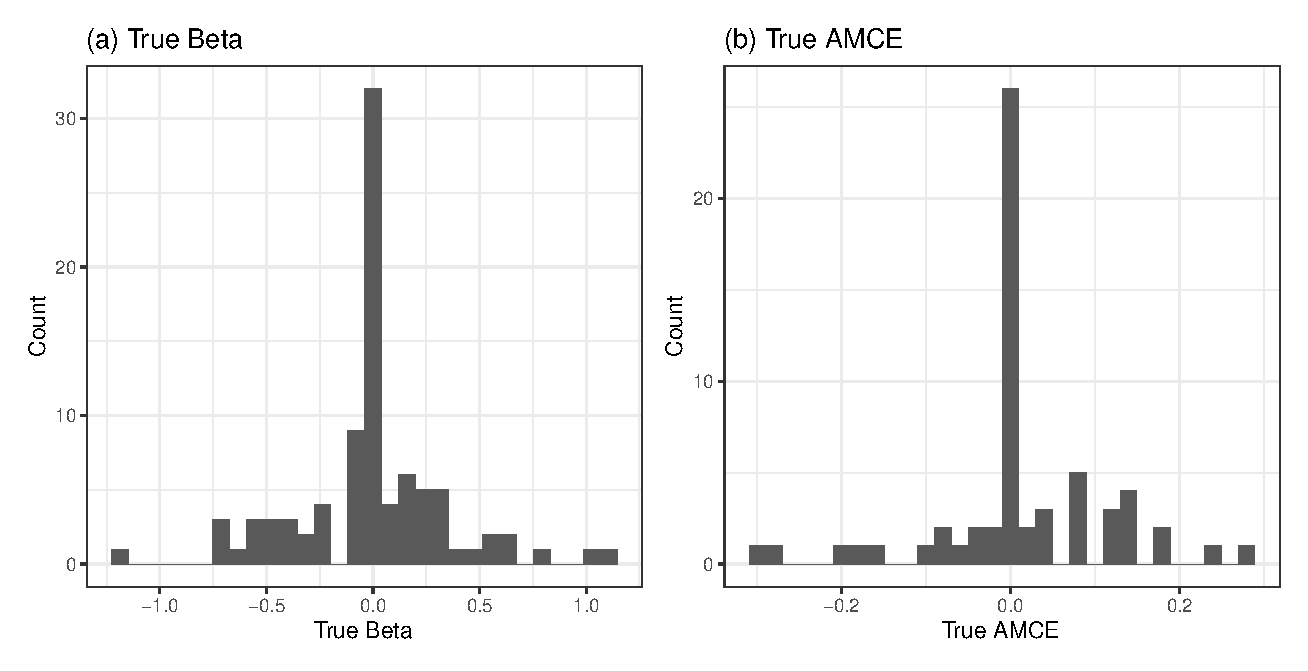
\includegraphics[width=\textwidth]{figures/sim_truth.eps}
\end{figure}

For each simulation, we draw $N'$ individuals who rate $T'$ profiles where $(N', T') \in \{(1000,5), (2000, 10)\}$. For each individual $i'$, we draw its moderators $\bm{x}_{i'}$ from a correlated multivariate normal where $\bm{x}_{i'} \sim N(\bm{0}_5, \bm{\Sigma})$ with $\bm{\Sigma}_{ij} = 0.25^{|i-j|}$ for $i,j \in \{1, \cdots, 5\}$. The distribution of cluster assignment probabilities $\pi_{ik}$ is shown below from one million Monte Carlo simulations of $[1, \bm{x}_{i'}^\top]$.

\begin{figure}[!htbp]
	\caption{Cluster Membership Probabilities}
	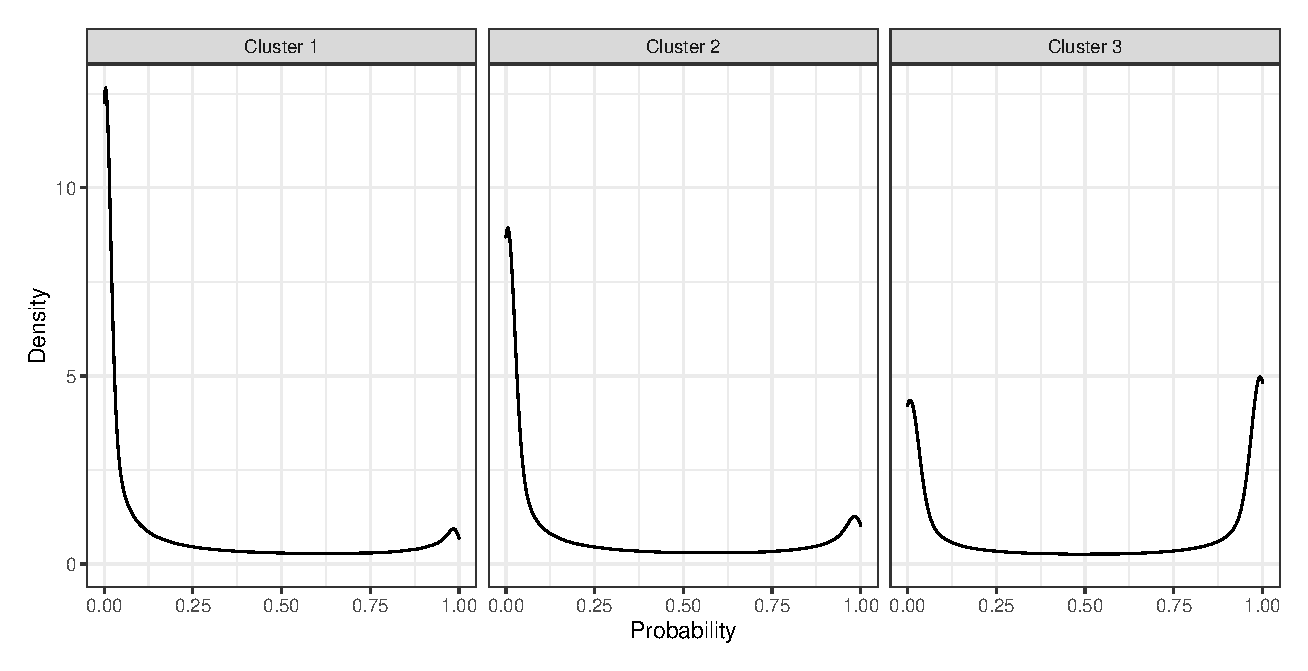
\includegraphics[width=\textwidth]{figures/sim_pi.eps}
\end{figure}

We see that the members are well-separated; the clusters are somewhat unbalanced, i.e. $\bar{\bm{\pi}} = [0.217, 0.261, 0.522]$. If we consider the maximum probability for each person $i$, i.e. $\pi^*_i = \max_{k \in \{1, 2, 3\}} \pi_{ik}$, this distribution has a median of 0.93, a 25th percentile of 0.75 and a 75th percentile of 0.99.

In terms of simulating the treatment profiles and outcome, for each individual $i'$, we draw their true cluster membership $z_i'$ using their $\bm{\pi}_{i'}$. For each task $t'$, we then draw a pair of treatments at random and then, given $z_i'$, draw the outcome $y_i'$ using the generative model outlined in the main text. 

After estimating our model with $K = 3$, we resolve the problem of label switching by permuting our estimate cluster labels to minimize the absolute error between the estimated posterior membership probabilities $\{E[z_{ik} | \bm{\theta}]\}_{k=1}^K$ and $\bm{z}_i'$ (the one-hot assignment of cluster membership).

\subsection{Additional Results}
\label{sec:app_simulations_coverage}

We provide additional simulations to complement the main text. Figure~\ref{fig:app_simulation_beta} presents the results for the simulations in the main text when considering the $\bm{\beta}_k$ (instead of the AMCE). It shows a similar story of some bias even at the larger sample size.

\begin{figure}[!ht]
	\centering \spacingset{1}
	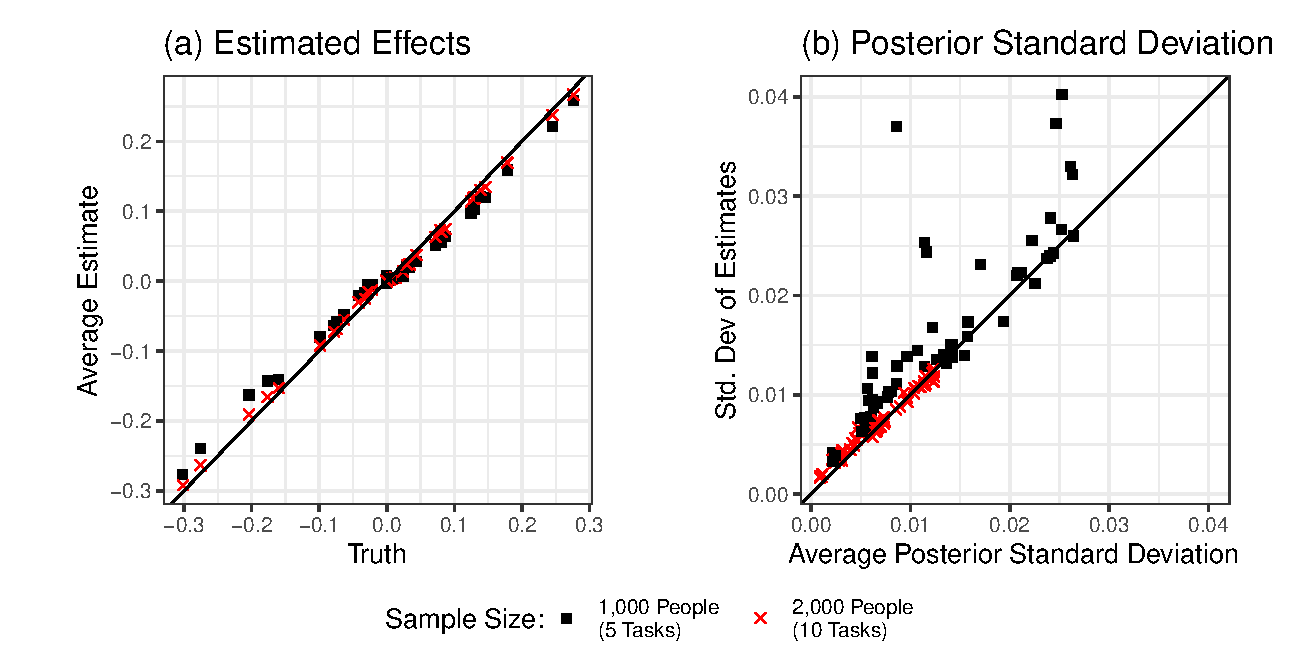
\includegraphics[width=\textwidth]{figures/sim_ame.eps}
	\caption{The empirical performance of the proposed estimator on
		simulated data. The black squares indicate the effects estimated
		with the smaller sample size (1,000 people completing 5 tasks);
		the red crosses indicate effects estimated with the larger sample
		size (2,000 people completing 10 tasks).}
	\label{fig:app_simulation_beta}
\end{figure}

To address this, we consider an alternative procedure employing sample splitting. We fit the model using half of the data (selected at random) and then refit the model. To refit the model, we hold fixed the sparsity pattern estimated in the original estimation holds (i.e., which levels are fused together) using a tolerance of $10^{-3}$. We also fix the estimated moderator relationship, i.e. $\pi_{k}(\bX_i)$, and only estimate the treatment effect coefficients after fusion. Algorithm~\ref{alg:refit} states the procedure. To calculate the average marginal effects, as noted in Appendix~\ref{append:amce_acie_der}, we use the empirical distribution of treatments to marginalize over other factors. In this split version, we also use the distribution from the full dataset.

\begin{algorithm}[!ht]\spacingset{1.25}
	\caption{Refitting Procedure}
	\label{alg:refit}
	\begin{algorithmic}
		\State{1. Randomly split the observations $i \in \{1, \cdots, N\}$ into two groups indexed by $\mathcal{I}_1$ and $\mathcal{I}_2$} 
		\State{2. Using the data $i \in \mathcal{I}_1$, estimate the parameters of the model using Algorithm~\ref{alg:main} in the main text. Define the resulting parameters from this as $\tilde{\bm{\theta}}$: $\{\tilde{\bm{\beta}}_k\}_{k=1}^K$, $\{\tilde{\bm{\phi}}_k\}_{k=2}^K,~\tilde{\mu}$}
		\State{3. Fuse levels $l$ and $l'$ of factor $j$ for cluster $k$ where the following condition holds for tolerance $\epsilon$
		
		$$\max \left\{\left|\tilde{\beta}^j_{kl} - \tilde{\beta}^j_{kl'}\right|\right\} \bigcup \left\{\bigcup_{j' \neq j} \bigcup_{m=0}^{L_{j'}-1} \left| \tilde{\beta}^{jj'}_{klm} - \tilde{\beta}^{jj'}_{kl'm}\right|\right\} \leq \epsilon$$
		
		For each combination where this is satisfied, construct matrices $\bm{R}_k$ that contain the required equality constraints, i.e. where $\bm{R}_k^T\tilde{\bm{\beta}}_k$ ensures that $\tilde{\beta}^j_{kl} = \tilde{\beta}^j_{kl'} = 0$ or $\tilde{\beta}^{jj'}_{klm} - \tilde{\beta}^{jj'}_{kl'm} = 0$. 
		
		Define $\tilde{\pi}_k(\bX_i)$ as follows:
		
		$$\tilde{\pi}_k(\bX_i) = \frac{\exp(\bX_i^\top \tilde{\bphi}_k)}{\sum_{k'=1}^K
			\exp(\bX_i^\top \tilde{\bphi}_{k'})}$$	
		}
		\State{4. Using the other half of the data $i \in \mathcal{I}_2$, estimate the refit parameters for the treatment effects, where $\bC$ contains the original sum-to-zero constraints discussed in the main text.
		\begin{equation*}
		\{\hat{\bm{\beta}}^{\mathrm{refit}}_k\}_{k=1}^K, \hat{\mu}^{\mathrm{refit}} = \argmax_{\{\bm{\beta}_k\}_{k=1}^K, ~\mu}~\sum_{i \in \mathcal{I}_2} \ln \left(\sum_{k=1}^K \tilde{\pi}_k(\bm{X}_i) \zeta_k(\bm{T}_i)\right) \quad \mathrm{s.t.} \quad \bC^T \bm{\beta}_k = \bm{0},~\bm{R}_k^T\bm{\beta}_k = \bm{0}
		\end{equation*}
		}
	\end{algorithmic}
\end{algorithm}

Figure~\ref{fig:app_dist_simulations} compares the estimators from the split sample and full data (``Full Sample'', i.e. the methods shown in the main text) approaches. It shows the distribution of the root mean-squared error (RMSE), bias, and coverage across the estimated AMCE and coefficients. We split the results by whether the true underlying effect is zero to compare differences across those cases. We also consider one even larger sample size (4,000 people with 10 tasks) to examine a scenario where the split sample method has the same amount of data as the full sample method for the second step in the estimation process.

\begin{figure}
	
	\begin{subfigure}{\textwidth}	
		\caption{Results for AMCE}
		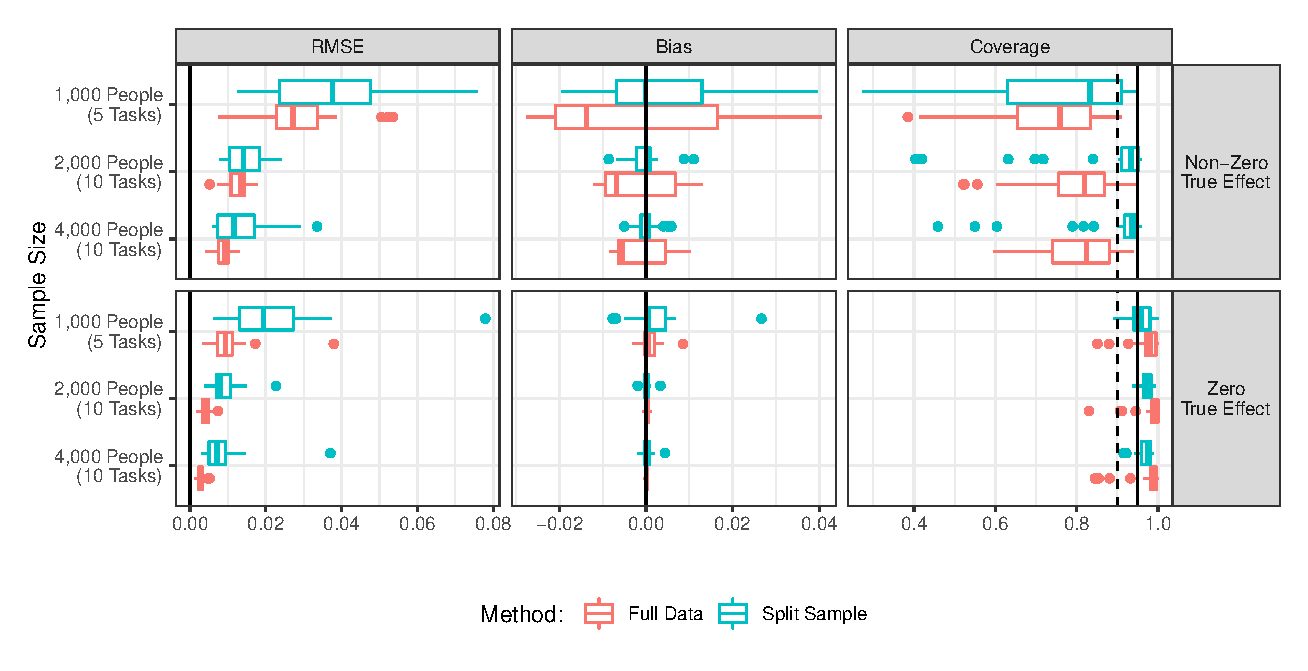
\includegraphics[width=\textwidth]{figures/app_perf_splitsample_ame.eps}
	\end{subfigure}

	\begin{subfigure}{\textwidth}	
			\caption{Results for $\bm{\beta}_k$}
			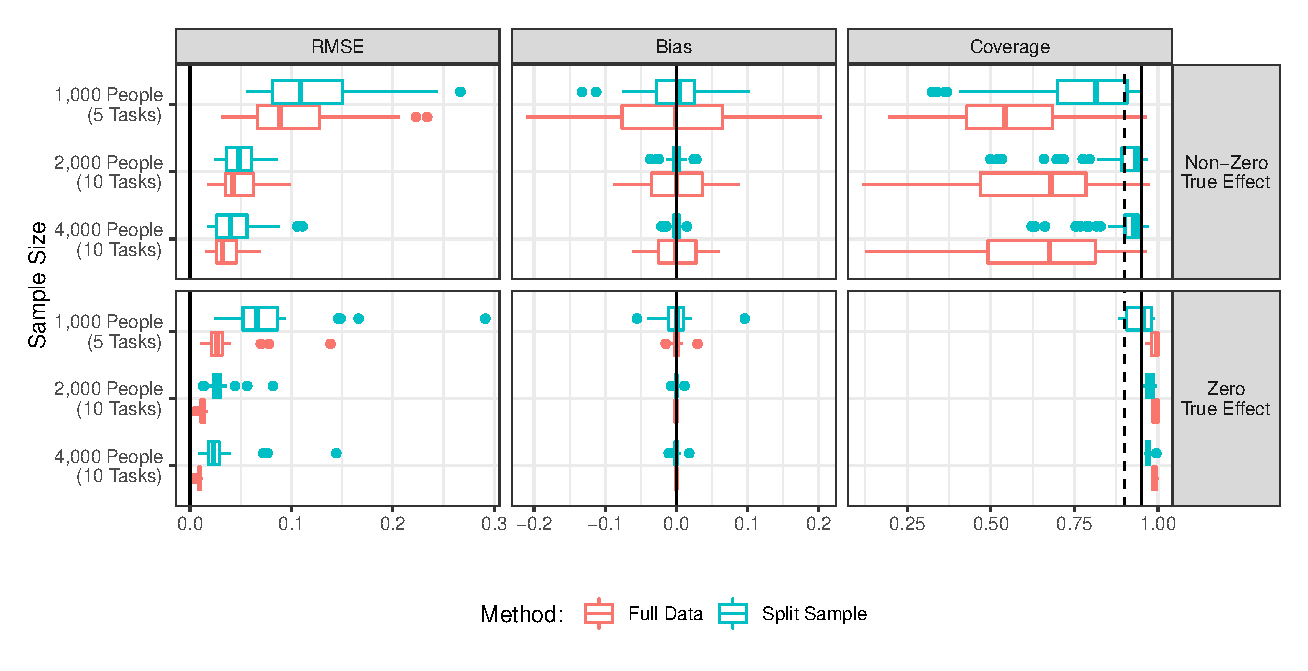
\includegraphics[width=\textwidth]{figures/app_perf_splitsample_beta.eps}
	\end{subfigure}

	\caption{The distribution of performance for each estimator across ample sizes. The top figure shows results for the AMCE; the lower figure shows results for the coefficients $\bm{\beta}_k$. Inside each figure, results are split by whether the true effect is zero (``Zero True Effect'') or not (``Non-Zero True Effect''). The boxplot shows the distribution across all effects for each cluster. For the plots on RMSE and bias, the solid vertical line indicates zero. For coverage, the solid line indicates 95\% coverage and the dashed line indicates 90\%.}\label{fig:app_dist_simulations}
\end{figure}

The figure corroborates the initial results that the full data method has non-trivial bias that decreases very slowly even at the largest sample sizes. By contrast, the bias is very small in the split sample method. As the panel on coverage shows, this results in considerably better coverage---especially for quantities with a non-zero true effect. At the two larger sample sizes, the median frequentist coverage of the split sample method is close to the nominal 95\%, with a few outliers that have low coverage. In terms of RMSE, the methods perform similarly.


\section{Additional Results for Immigration Conjoint Experiment}
\label{app:emp_marg_means}

We provide some additional results for our main empirical analysis. First, focusing on the three-cluster model, we report a different quantity of interest. We use an analogue to the ``marginal means'' estimator in \cite{leeper2020measuring}. We compute the probability of a profile being chosen \emph{without} specifying a baseline category. The equation is shown below for the forced choice case; note it consists of two of the terms used for the AMCE. 

\begin{align}
\mathrm{MM}_{jk}(l) & \ = \ \frac{1}{2}\E \left[
\left\{\Pr\left(Y_i = 1 \mid Z_i=k, T^L_{ij}=l,
\bT^L_{i,-j}, \bT^R_{i}\right) + \Pr\left(Y_i = 0 \mid Z_i=k, T^R_{ij}=l,
\bT^R_{i,-j}, \bT^L_{i}\right)
\right\}\right]. 
\end{align}

The below plot ignores randomization restrictions when estimating this quantity to center the estimate around 0.50 as in \cite{leeper2020measuring}. The results are substantively similar to the analysis in shown in the main paper using AMCEs.

\begin{figure}[t!]
	\centering \spacingset{1}
	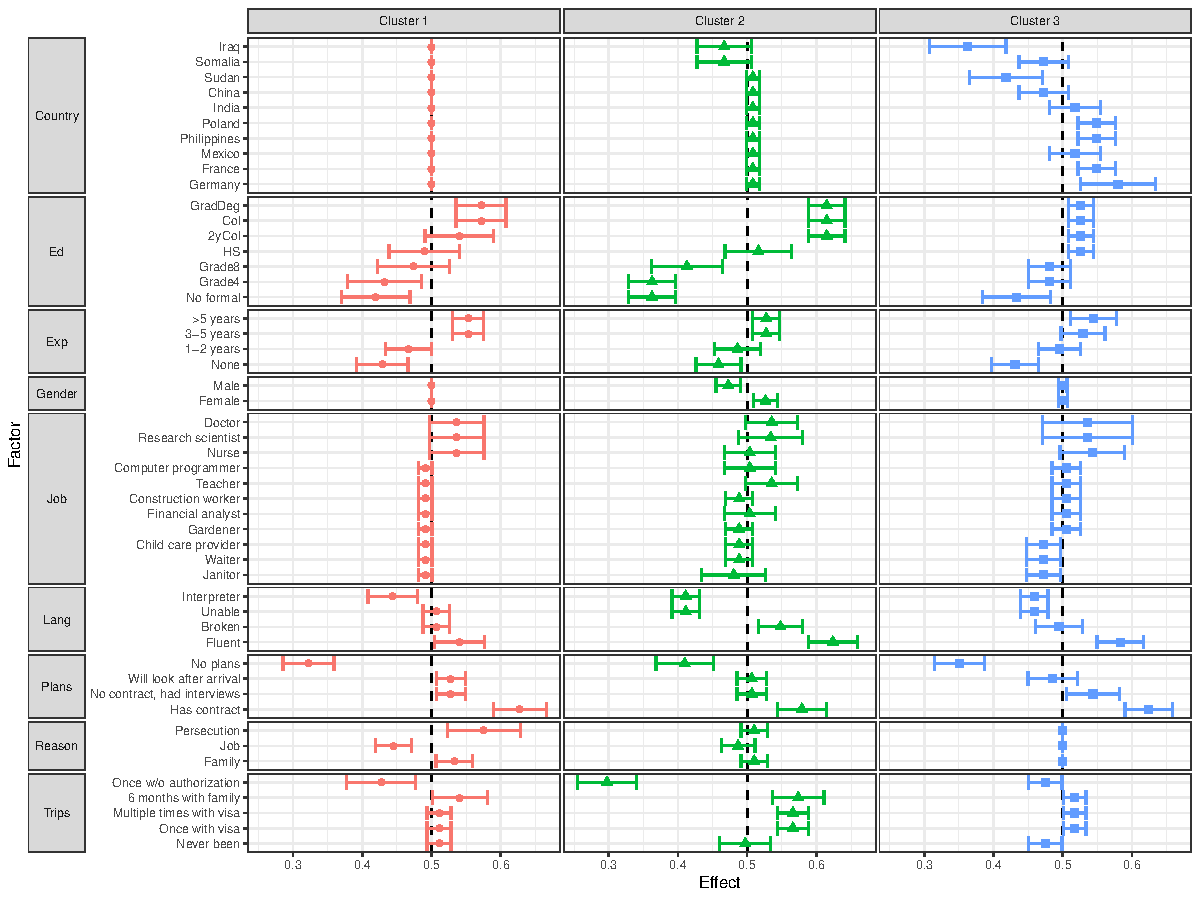
\includegraphics[width=\textwidth]{figures/marginal_means.pdf}
	%6x8
	\caption{Estimated average marginal means using a
		three-cluster (right) analysis. The point
		estimates and 95\% Bayesian credible intervals are shown.} \label{fig:marg_means}
\end{figure}

Second, as noted in the main text, we found that sample splitting and refitting the model (see Appendix~\ref{sec:app_simulations_coverage}) was somewhat unstable given different splits of the data. To illustrate this point, Figure~\ref{fig:perm_AMCE} shows the 25th-75th percentile (and median) of the AMCEs estimated across twenty repetitions of splitting the data into halves and then using the refitting procedure described above. We address the problem of label switching using a permutation of labels that minimizes the average mean absolute error between all pairs of estimates; we find a permutation by randomly permuting the labels for a randomly chosen set of estimates and repeat this repeatedly until the average mean absolute error stabilizes. 

While Figure~\ref{fig:perm_AMCE} shows instability in some of the estimated AMCE, it broadly shows a similar result to that in the main text. For example, one cluster (Cluster 2 when $K=2$; Cluster 3 when $K=3$) shows a clear effect of country across most splits whereas one cluster (Cluster 1 when $K=2$ and Cluster 2 when $K=2$) generally shows a large penalty for immigrants who entered without legal authorization. 

\begin{figure}[!htbp]
	\centering \spacingset{1}
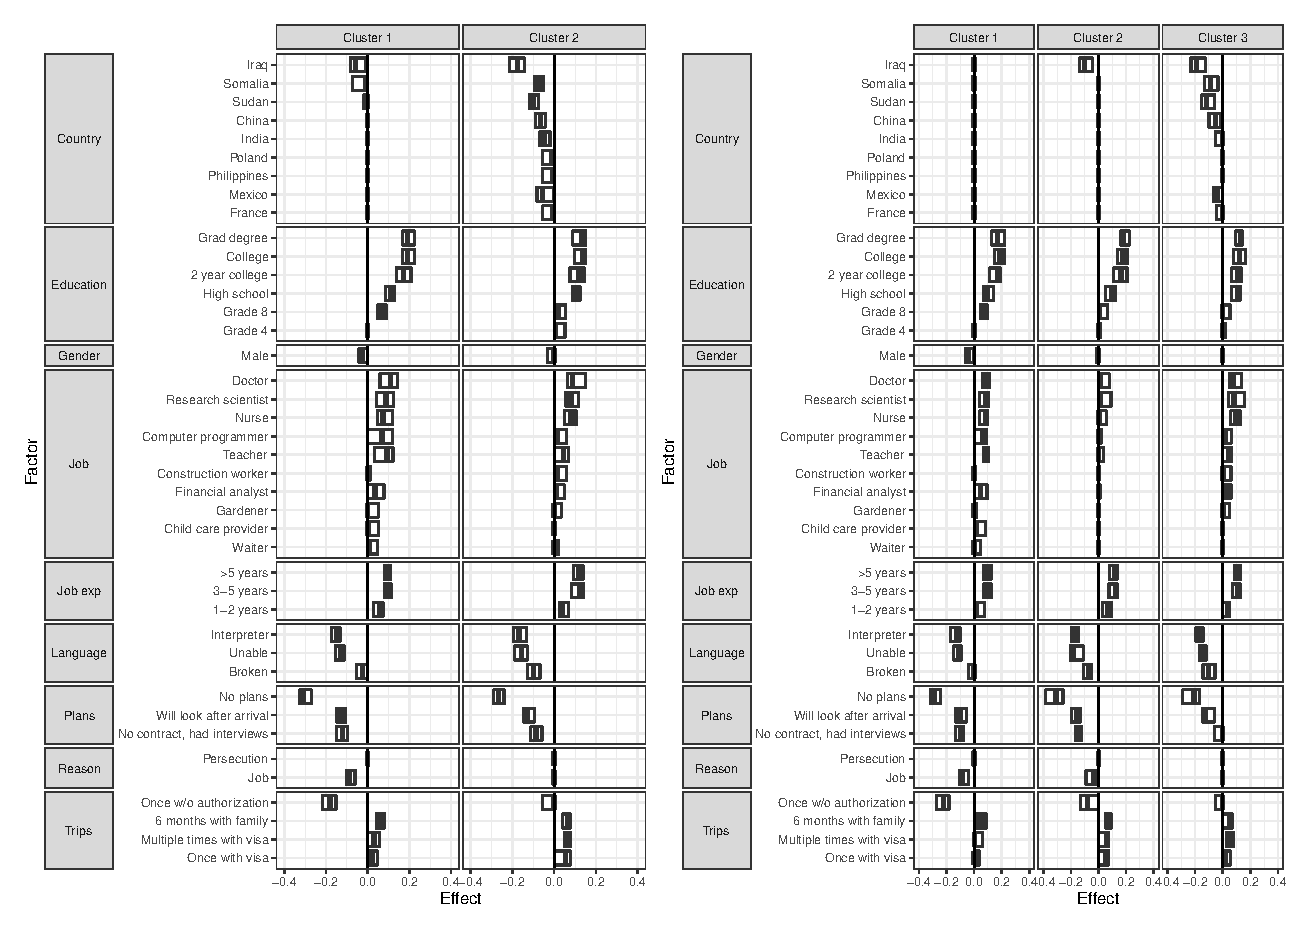
\includegraphics[width=\textwidth]{figures/app_repeat_hh_AME.eps}
%6x8
\caption{The distribution of AMCE from a two-cluster and three-cluster model with twenty random splits of the data. The interquartile range and median are shown.} \label{fig:perm_AMCE}
\end{figure}

	\end{set11}
\end{appendices}

\end{document}

